\afterpage{\blankpage}

\chapter{Introdução}
\label{cap:intro} 
\setcounter{page}{29}

A História da Arte costuma ser dividida em períodos, tendências,
escolas, estilos e mais recentemente, em movimentos
artísticos.~\cite{dempsey} Um período compreende o limite de tempo
onde certas características predominam entre as obras. Também, em um
dado período, há o desenvolvimento de tendências: características na
linguagem artística (i.e.\ cores, texturas, materiais, composições)
que tornaram-se marcantes e serão transmitidas para as próximas
gerações, seja por sua afirmação ou refutação. Essas tendências, ao se
consolidarem, compõem escolas ou estilos. Os movimentos artísticos
também apresentam ideias e características comuns, mas costumam ter
bem definidos: sua data de criação, local, participantes, assim como
um manifesto.

Seja qual for a classificação tomada para a história da Arte e de seus
artistas em termos de movimentos e períodos, é possível perceber algo
latente: as características de suas obras estão em constante
transformação, definindo os diferentes períodos ou escolas. A história
da Arte é portanto permeada por uma sucessão de similaridades e
oposições destas características ou ideias. A Pintura oferece inúmeros
exemplos. Brunelleschi e Alberti inauguraram um estilo de
pintura~\cite{andersen,kemp} onde conseguiam representar a
profundidade visível de uma cena utilizando um método geométrico:
linhas paralelas convergindo em um ou mais pontos no horizonte.
(figura~\ref{fig:perspectiva}). Até então as pinturas, afrescos,
mosaicos e desenhos não tinham noção alguma de profundidade --- os
elementos que compunham a pintura eram distribuídos segundo sua
importância espiritual ou temática,~\cite{edgerton} utilizando, por
exemplo, a simples sobreposição dos elementos na tela. Esse estilo
acabaria por fazer parte das características da grande maioria das
pinturas a partir do século XV.~\cite{gombrich} Porém, ela não foi
suficiente para Cézanne nem seus contemporâneos da Arte Moderna, que
estavam descontentes com essa ``equação matemática'' e usaram
gradações de cores para representar a profundidade, rompendo com a
tradição iniciada por Brunelleschi e Alberti.~\cite{sedlmayr}

\begin{figure}[h!]
  \begin{center}
\caption{A imagem superior é a ilustração ``Reconstrução do
        Templo de Jerusalém'' (1200-1300) para o livro
        ``\textit{Histoire d'Outremer}'', de Guilherme de Tiro. Esta
        pintura antecede o método de perspectiva de Brunelleschi e
        portanto é possível notar a ausência de linhas que convirjam
        para um só ponto, embora haja a intenção da representação de
        profundidade, pela sobreposição dos elementos. Já a imagem
        inferior, um afresco de Pietro Perugino (1481-1482), apresenta
        o estilo de perspectiva, com todas as linhas convergindo para
        o centro da imagem, em seu horizonte. As imagens ilustram como
        o estilo pode influenciar mudanças nas características das
        obras ao longo da história.}
    \label{fig:perspectiva}
    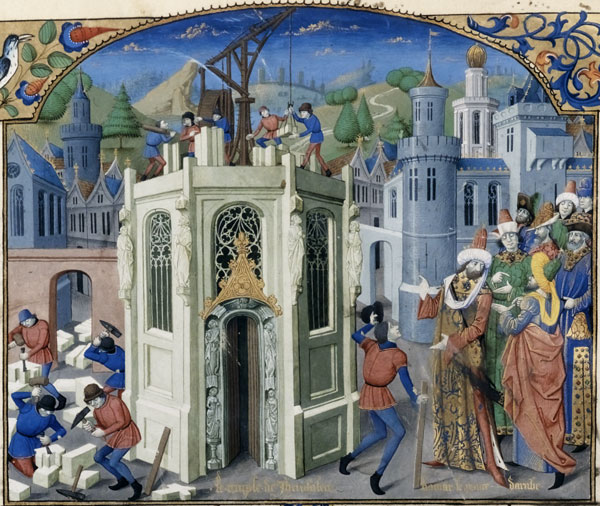
\includegraphics[width=0.6\textwidth]{figs/perspectiva1.png} \\
    \vspace{1cm}
    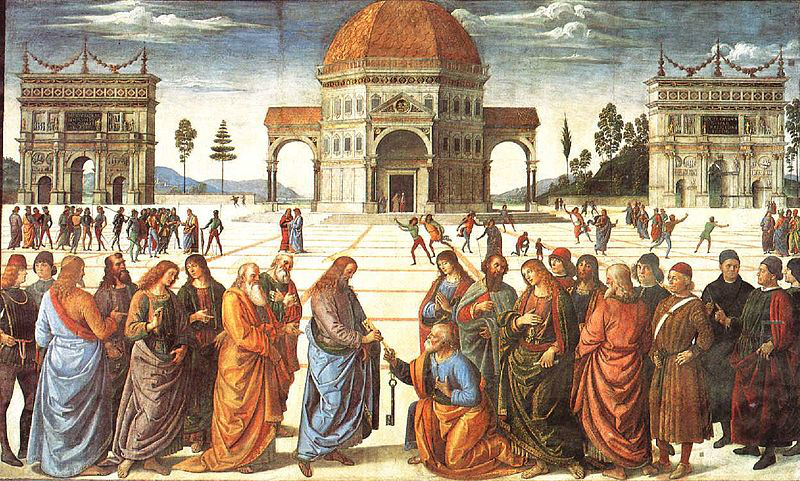
\includegraphics[width=0.6\textwidth]{figs/perspectiva2.png}
      \fonte{figperspec}
      
\end{center}
\end{figure}

A ``Monalisa'' de Leonardo da Vinci~\cite{pegus, hall} é um dos
principais exemplos do estilo \textit{sfumato}, onde as pinceladas que
definem bordas e linhas são removidas com verniz de madeira, comum nas
pinturas renascentistas. Outros estilos de pintura como as cores da
Escola de Viena,~\cite{gardner} o movimento e a
expressão,~\cite{gombrich, gordon} foram criados por cada geração de
artistas em uma tentativa de expressar as características que
desejavam. A cada geração, estes mesmos artistas descobriram que
continuavam existindo convenções que os obrigavam a aplicar o que
haviam aprendido ao invés de pintarem o que realmente viam. Os
``rebeldes'' da Arte Moderna acabaram por negar essas convenções,
criando novos meios. Van Gogh não estava interessado em seguir
estritamente as regras da perspectiva e profundidade, ao invés disso,
deformava a imagem para ressaltar detalhes que lhe eram
relevantes. Picasso não se importava que o resultado final de sua obra
parecesse distante do modelo original, e desta forma sentia-se livre
para retratar verdadeiras colagens das várias perspectivas possíveis
do modelo, todas sobrepostas na mesma pintura. Miró pintava símbolos
baseando-se em um dicionário que criara, sendo um dos primeiros a
utilizar a pintura automática. O século XX presencia a passagem de uma
geração de experimentadores, inventores, que davam maior preferência à
originalidade do que à tradição. Não queriam mais a ``fidelidade'' de
Caravaggio ou a ``beleza ideal'' de Poussin, buscavam ``expressividade
intensa, clareza de estrutura e uma simplicidade linear na
técnica.''~\cite{gombrich} No modernismo não existiam estilos
predominantes --- como no caso do período Barroco --- mas existiam sim
várias abordagens, criadas ou desenvolvidas por cada artista. Como bem
dito por Gombrich:~\cite{gombrich} ``Qualquer afastamento da tradição que
interessasse à crítica e atraísse um seguidor era saudado como um novo
\emph{ismo} ao qual o futuro pertenceria''. Essa inquietação moderna é
avistada nas linhas retas e arquitetura funcional das casas e prédios
do outro lado da rua, apenas para citar uma das influências que a Arte
Moderna acabou por tornar presente no dia-a-dia.

É justamente essa sucessão de oposições e similaridades entre
características nas obras artísticas que torna este estudo
possível. Nele, busca-se entender essa evolução de uma maneira
quantitativa, através de medidas geométricas. Estas medidas têm como
base conceitos centrais no estudo da Filosofia: \textit{oposição},
\textit{inovação} e \textit{dialética}.~\cite{deleuze,pinto,van} A
dialética por exemplo é definida como um método de argumentação onde
busca-se a síntese entre dois argumentos contraditórios: a tese e a
antítese. São conceitos originalmente qualitativos. Neste estudo, aqui
apresentado, promove-se um ponto de vista alternativo: tese, antítese
e síntese são definidas como estados em uma série temporal. A
dialética torna-se uma medida quantitativa: o inverso da distância
entre o estado da síntese e a mediatriz formada pelos estados de tese
e antítese. Quanto menor a distância, maior a dialética, pois o estado
de síntese se aproxima da mediatriz, que representa no espaço vetorial
o que seria a síntese ideal entre as ideias de tese e
antítese. Pode-se, assim, medir
\emph{quanto} um argumento apresenta de dialética. Ou se um dado
argumento possui dialética maior ou menor que outro, apresentando para
isso, valores numéricos. Essas medidas são discutidas de maneira
extensiva na seção~\ref{sec:medidas}.

Para ser possível tal análise, é necessária a representação dos
agentes envolvidos --- nesse caso, pintores e suas obras --- em um
espaço vetorial onde as medidas são então realizadas. Esse mapeamento,
das imagens de pinturas para o espaço vetorial, começa com a seleção
de imagens das pinturas. Para os resultados obtidos no estudo aqui
apresentado, foi selecionado um grupo de 12 pintores: 6 do período
Barroco e outros 6 de movimentos da Arte Moderna. A escolha de grupos
com tamanha disparidade cronológica tem seu motivo: a História da Arte
reconhece diferenças contrastantes entre o período Barroco e os vários
movimentos da Arte Moderna, porém tais afirmações são
qualitativas. Neste estudo, busca-se afirmar ou refutar estas
afirmações com base em medidas quantitativas. Um total de 20 pinturas
de cada autor foi escolhido aleatoriamente, formando um conjunto de
240 pinturas analisadas. Métodos de processamento de imagens foram
aplicados para extrair atributos que caracterizam cada
pintura. Através da análise de matriz de espalhamento e LDA
(\textit{Linear Discriminant Analysis}),~\cite{luciano,fisher} os
atributos que melhor classificaram as pinturas em seus respectivos
pintores foram selecionados. Esses vetores de atributos, agora com
dimensões reduzidas, formam então o espaço vetorial
pretendido. Considerando tais vetores em ordem cronológica, tem-se uma
série temporal e é nessa série que se dá o cálculo das medidas
sugeridas para a oposição, inovação e dialética.

Enquanto valores numéricos, tais medidas revelam padrões que encontram
paralelo na história da Arte. Um exemplo marcante é o contraste entre
pintores barrocos e modernos. Enquanto todo o grupo Barroco apresenta
sobreposição entre seus pintores, o grupo de pintores modernos
apresenta quase nenhuma sobreposição. Essa observação encontra base na
história da Arte, onde os pintores barrocos, reconhecidamente,
compartilham técnicas uns com os outros --- e portanto, compartilham
também características estéticas em suas pinturas --- enquanto os
modernos são marcados pelo individualismo, cada qual definindo seu
próprio estilo.

As medidas, assim como o método de análise de séries temporais, são
independentes de domínio, o que possibilita sua aplicação para a
análise de outras áreas além da Pintura. Até então, Filosofia,
Música~\cite{vieira} e Pintura foram avaliadas. Aplicações em Cinema,
Literatura e Arquitetura, por exemplo, são possíveis. Tal
flexibilidade permite também a comparação entre as medidas obtidas
para cada área de conhecimento. Por exemplo, é possível notar que na
Música há predomínio de valores altos para a dialética, enquanto na
Filosofia, a oposição é o caráter predominante.~\cite{vieira} Já na
Pintura, há constante inovação, e ambas oposição e dialética possuem
maior valor no momento de transição de um movimento artístico ao
outro. Novamente, cada um desses resultados encontra fundamento na
história e nas características de cada um de seus autores e
obras. Tais resultados, sugerem evidências quantitativas da tradição
mestre-aprendiz encontrada na Música e tradição de oposição encontrada
na Filosofia. Estas tradições são plenamente reconhecidas nas áreas de
Música e Filosofia.~\cite{vieira} Na Pintura, verifica-se constante
inovação, enquanto oposição e dialética são fortes somente no momento
de transição entre períodos artísticos, o que pode vir a acrescentar à
compreensão histórica das Artes Plásticas.

\section{Motivação}

A subjetividade da história das artes sugere métodos mais objetivos de
análise. É importante ressaltar que o método aqui apresentado não
pretende esgotar ou suplantar a análise subjetiva, humana, mas sim
complementá-la, somar ao ferramental metodológico já existente. Da
mesma forma, conceitos como a dialética possuem grande importância nas
Ciências Humanas, mas são comumente tratados de maneira qualitativa.

Ainda, o cálculo automático dos atributos usados para análise também
motivou esse estudo. No estudo anterior,~\cite{vieira} os atributos
eram fornecidos por críticos (os próprios autores) através de notas
dadas a uma determinada característica de uma obra. No caso da Música,
complexidade rítmica, número de vozes e harmoniosidade dos timbres, são
exemplos de características consideradas. Na Filosofia, exemplos de
características que foram consideradas são: reducionismo/holismo,
teocentrismo/antropocentrismo e racionalismo/empirismo. Na busca pela
automatização, fez-se uso do processamento de imagens para extrair
atributos das pinturas. Procura-se assim investigar se na Pintura
haveriam similaridades com as áreas já analisadas (Música e
Filosofia).

\section{Objetivos}

O objetivo principal deste trabalho é modelar artefatos produzidos por
artistas como um conjunto de características projetadas em um espaço
vetorial. Assim, é oferecida uma forma complementar à interpretação da
história artística. Conceitos subjetivos --- antes apenas de domínio
das Ciências Humanas --- como dialética, oposição e inovação podem ser
calculados como medidas quantitativas.

\section{Organização}

No capítulo~\ref{cap:fundamentos} são descritos os fundamentos,
algoritmos, métodos canônicos e detalhes históricos sobre os quais se
construiu este estudo, assim como trabalhos relacionados e de
interessante leitura. No capítulo~\ref{chap:resultados} são apresentados os
desenvolvimentos realizados nesse estudo: o processamento de imagens
para obtenção das características, a representação da evolução
artística em um espaço vetorial e a interpretação das medidas de
dialética, oposição e inovação. Os resultados são confirmados pelo
cálculo dos componentes que mais separam os grupos de pintores,
através do método LDA. Este, por sua vez, é validado por uma matriz de
confusão. Por fim, no capítulo~\ref{chap:conclusoes} há uma revisão do
que foi discutido e são apontadas as principais contribuições e conclusões
desse estudo, além de refletir sobre desenvolvimentos futuros e que já
estão em andamento. No apêndice~\ref{cap:ap-tutorial} é apresentado um tutorial
para \textit{download} e execução dos \textit{scripts} em linguagem de
programação \textit{Python} que implementam os algoritmos
desenvolvidos para essa análise. No apêndice~\ref{cap:ap-galeria} há uma galeria com as
240 imagens das pinturas usadas no estudo. No apêndice~\ref{ap:alternativa} é apresentada
uma visualização alternativa da série temporal resultante, que também
pode ser explorada através de um aplicativo Web interativo. No apêndice~\ref{ap:sifisc} são descritas as contribuições artísticas deste estudo: uma exposição
realizada em 2013 no IFSC/USP com imagens geradas a partir de um
algoritmo desenvolvido para pintura generativa.

%%%%%%%%%%%%%%%%%%%%%%%%%%%%%%%%%%%%%%%%%%%%%%%%%%%%%%%%%%%%%%%%%%%%%%%%%%%
%%%%%%%%%%%%%%%%%%%%%%%%%%%%%%%%%%%%%%%%%%%%%%%%%%%%%%%%%%%%%%%%%%%%%%%%%%%

\afterpage{\blankpage}
\chapter{Fundamentos}
\label{cap:fundamentos}

Neste capítulo são descritos os fundamentos, algoritmos e métodos
canônicos, com os quais se realizou esta pesquisa. A
seção~\ref{sec:breve} apresenta um resumo sobre características
encontradas em ambos períodos Barroco e Moderno, assim como uma
pequena biografia de cada artista selecionado para este estudo. A
seção~\ref{sec:fund:filosofia} revisa os conceitos de oposição,
inovação e dialética. Estes conceitos foram emprestados da Filosofia e
tornados medidas quantitativas, discutidas na seção~\ref{sec:medidas}.

Os momentos estatísticos básicos, usados ao longo de todo o estudo,
são revisados na seção~\ref{sec:momentos}. A
seção~\ref{sec:fund:imagens} apresenta os métodos de processamento de
imagens usados neste estudo para extrair vetores de características
das pinturas, definidos na seção~\ref{sec:atributos}. A
seção~\ref{sec:fund:reducao} encerra este capítulo com a discussão do
método de espalhamento de matrizes, usado para identificar quais
vetores de atributos mais contribuíram para a \textit{clusterização}
das pinturas, assim como o método LDA, que foi aplicado para a redução
das dimensões da matriz de atributos. O método LDA confirmou os
resultados obtidos para o melhor par de atributos.

\section{Uma breve introdução ao Barroco e Arte Moderna}
\label{sec:breve}

É interessante levantar aqui algumas características sobre a história
e estética do período Barroco e de movimentos da Arte Moderna. Tais
pontos, relacionados diretamente às Artes Plásticas, estão sumarizados
na seção~\ref{subsec:sumario} e serão confrontados com observações
obtidas pela análise das medidas quantitativas, discutidas na
seção~\ref{sec:pares}. O resumo biográfico de cada artista
considerado, auxilia na avaliação de tais resultados.

\subsection{Barroco}

O Barroco na pintura é marcado pela tradição, pelo desejo de retratar
a verdade (encontrado nas obras de Caravaggio, Frans Hals e
Velázquez), a beleza (em Poussin, Vermeer), o sagrado (Caravaggio,
Rembrandt). Esteticamente, é notável o uso do contraste de luz para
dar destaque a um determinado local da pintura enquanto escurece
regiões menos importantes, como na técnica do \textit{chiaroscuro}
de Caravaggio. Há também a preferência por oposições complexas e
desprezo pelo equilíbrio simplista na composição dos elementos em uma
pintura. Tais estéticas objetivam causar emoções em quem contempla os
quadros, geralmente de caráter sagrado, retratando passagens bíblicas
com grande fidelidade aos detalhes. A transmissão dessas técnicas ou
estéticas de um pintor para o outro é comum no Barroco. Espera-se,
portanto, que pintores barrocos apresentem uma grande similaridade
estética em suas obras.~\cite{gombrich,hills,gardner} Para o presente
estudo, os seguintes pintores foram escolhidos por representarem,
reconhecidamente, características do período Barroco:

\textbf{\emph{Miguel Ângelo da Caravaggio}}, Itália, 1573-1610.  Após
a Renascença, foram Annibale Carracci e Miguel Ângelo da
Caravaggio~\cite{bayer} que, mesmo tendo métodos completamente
opostos, amplificaram as ideias já apresentadas em Tintoretto e El
Greco durante o chamado Maneirismo:~\cite{tatarkiewicz} ênfase sobre
luz e cor, desprezo pelo simples equilíbrio, preferência por oposições
complexas. Tais ideias foram apresentadas de uma nova maneira e
inauguraram o que viria a ser o período Barroco.~\cite{hills}
Caravaggio --- diferente de Carracci que se preocupava em retratar o
belo --- queria retratar a verdade, como a via, em detalhes. Essa
busca pela verdade pode ser vista em
\emph{Judite e Holoferne} (figura~\ref{fig:caravaggio:judite}).~\cite{puglisi,caravaggio} 

\begin{wrapfigure}[10]{r}{0.5\textwidth}
  \vspace{-15pt}
  \begin{centering}
    \caption{\emph{Judite e Holoferne} (Caravaggio), c. 1599}
    \label{fig:caravaggio:judite}
    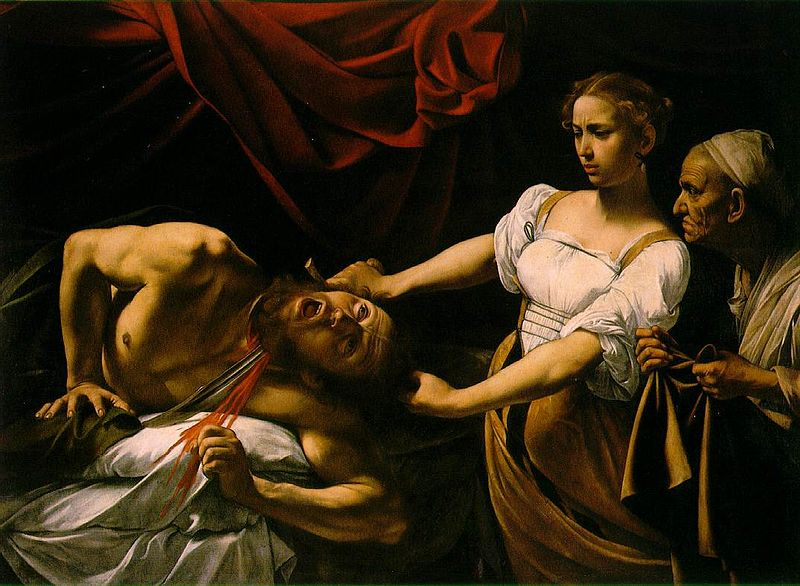
\includegraphics[width=0.5\textwidth]{figs/caravaggio_judite.png}
    \fonte{figcaravaggio}
  \end{centering}
\end{wrapfigure}

O uso da luz, contrastando rigidamente com o negro fundo, colabora
para ressaltar a jovialidade de Judite, que demonstra ter convicção do
que faz: cortar a cabeça de Holoferne. Sua serva por outro lado,
demonstra nervosismo, esperando que o pedaço de carne morta encha o
saco de pano que segura. É possível sentir o horror, a surpresa e
impotência de Holoferne enquanto é arrancado de seu sono por sua
própria espada. Caravaggio fornece assim uma interpretação de notável
detalhismo da passagem bíblica: ``Então Judite se aproximou da coluna
da cama, que ficava junto à cabeça de Holoferne, e pegou a espada
dele. Depois chegou perto da cama, agarrou a cabeleira de Holoferne, e
pediu: Dá-me força agora, Senhor Deus de Israel. E com toda a força,
deu dois golpes no pescoço de Holoferne e lhe cortou a cabeça. Rolou o
corpo do leito e tirou o mosquiteiro das colunas. Depois saiu,
entregou a cabeça de Holoferne para a serva, que a colocou na sacola
de alimentos.'' (Judite 13, 6)

\textbf{\emph{Frans Hals}}, Holanda, 1580(?)-1666. Ao mesmo tempo que o
Barroco era iniciado na Itália, que compreendia a metade católica da
Europa, em regiões protestantes como a Holanda, não havia espaço para
pintar o sagrado.~\cite{gombrich} Sobravam os retratos como fonte de
renda e Frans Hals~\cite{grimm} soube bem como pintá-los, embora
recebendo pouco em retorno. Sua obra é constituída em grande parte por
retratos de burgueses e mercadores Holandeses, como o \textit{Retrato
de Isaak Abrahamsz Massa} (figura~\ref{fig:hals:massa}), mercador e
amigo próximo de Hals. 

\begin{wrapfigure}[14]{l}{0.5\textwidth}
  \vspace{-15pt}
  \begin{centering}
    \caption{\emph{Retrato de Isaak Abrahamsz Massa} (Frans Hals), c. 1626}
    \label{fig:hals:massa}
    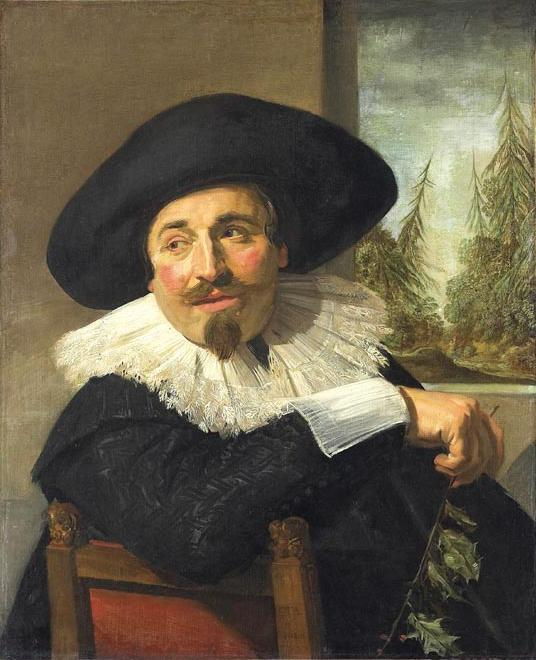
\includegraphics[width=0.5\textwidth]{figs/hals_massa.png}
    \fonte{fighals}
  \end{centering}
\end{wrapfigure}

Embora na época a maioria dos pintores e
estudantes estivessem influenciados pela técnica
do \textit{chiaroscuro} de Caravaggio, isso não se observa em Frans
Hals: o fundo possui detalhes, complementa a composição e existem
variações de sombra na face do modelo (o lado direito é iluminado por
uma luz direta, enquanto o lado esquerdo apresenta uma sombra de luz
natural). Em Caravaggio, a luz é outra, ela é direta, penetrante,
artificial.~\cite{gombrich} Ao mesmo tempo, os retratos de Frans Hals
diferiam dos retratos de até então. Sua pincelada rápida permitia
capturar não o modelo, mas o momento, o instante.~\cite{peter} Outra
diferença é a pose alternativa para a época. Diferente dos retratos
com olhares perdidos, Frans Hals usa os olhos do modelo para expressar
e compor o momento. Ao invés de um olhar perdido, Massa olha para algo
que lhe chama atenção, a ponto de virar-se na cadeira.

\textbf{\emph{Nicolas Poussin}}, França, 1594-1665. Carracci, Reni e
seus seguidores retratavam uma versão ``embelezada'' da natureza, que
imitava as estátuas clássicas. Este programa ficou conhecido como
neoclássico ou ``acadêmico.''~\cite{gombrich} Poussin foi um dos
grandes mestres ``acadêmicos'', influenciado pelo pintor que
representa a oposição a Caravaggio: Carracci. Suas pinturas querem
retratar a beleza, a inocência, a pureza de épocas antigas, seus mitos
e histórias.~\cite{unglaub} É possível notar essa intenção na
figura~\ref{fig:poussin:danca} que retrata sua obra \textit{Uma Dança
para a Música do Tempo}. 

\begin{wrapfigure}[10]{r}{0.5\textwidth}
  \begin{centering}
    \caption{\emph{Uma Dança para a Música do Tempo} (Nicolas Poussin), c. 1634-1635}
    \label{fig:poussin:danca}
    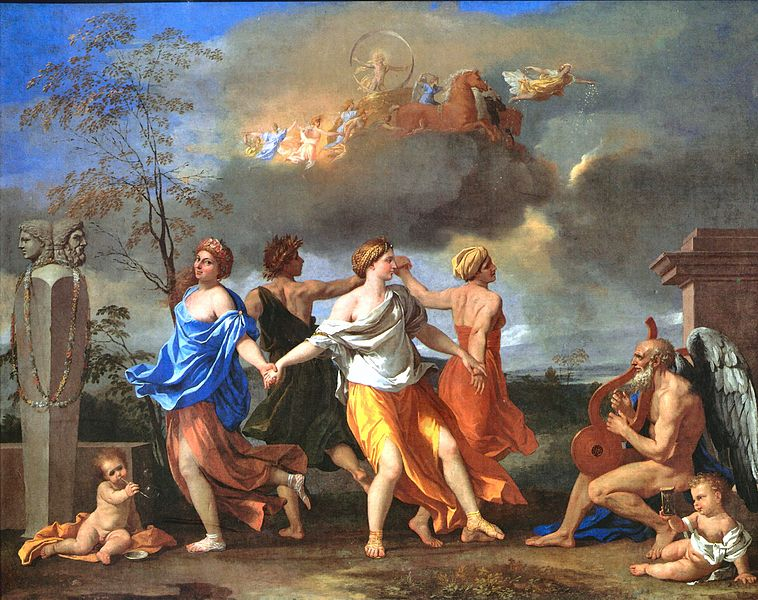
\includegraphics[width=0.5\textwidth]{figs/poussin_danca.png}
    \fonte{figpoussin}
  \end{centering}  
\end{wrapfigure}

É interessante apontar a diferença com a obra de Caravaggio e a
proximidade com as pinturas de Carracci ou Reni. Ao invés do fundo
escuro, da luz artificial, encontra-se uma paisagem iluminada, que se
preocupa em retratar o belo. Não há espaço para o horror, para a
rigidez da verdade, como acontece com Caravaggio.

% TODO: talvez incluir algumas pinturas de Carracci e Reni para facilitar
% a comparação

\textbf{\emph{Diego Velázquez}}, Espanha, 1599-1660. \\ Mesmo ainda não tendo
visitado Roma, Velázquez havia conhecido e se impressionado pelos
trabalhos de Caravaggio. Há grande semelhança entre suas obras e as
pinturas do mestre italiano, como é possível observar na
figura~\ref{fig:velazquez:velha} da obra
\textit{Velha Fritando Ovos}.

\begin{wrapfigure}[10]{r}{0.5\textwidth}
  \vspace{-45pt}
  \begin{centering}
    \caption{\emph{Velha Fritando Ovos} (Diego Velázquez), c. 1618}
    \label{fig:velazquez:velha}
    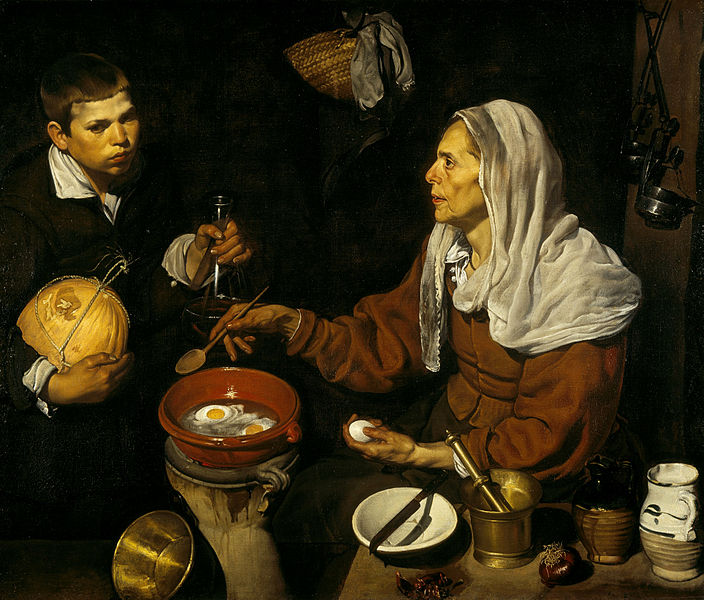
\includegraphics[width=0.5\textwidth]{figs/velazquez_velha.png}
    \fonte{figvelazquez}
  \end{centering}
\end{wrapfigure}

Assim como Caravaggio, retrata a natureza como ela é, sua verdade é
mais importante do que sua aparente beleza. Na pintura em destaque, há
uma grande preocupação com os detalhes: os ovos, as mãos, as feições
dos modelos, os utensílios de cozinha, o vidro que o menino segura,
todos representados com precisão fotográfica. A técnica do
\textit{chiaroscuro} de Caravaggio foi aplicada, onde uma luz intensa à
esquerda da pintura ilumina com grande contraste os detalhes que
Velázquez queria propositalmente ressaltar. Ao mesmo tempo, o fundo é
tão negro que não se pode mais observar as paredes do
ambiente.~\cite{gombrich}

\begin{wrapfigure}[13]{r}{0.4\textwidth}
  \begin{centering}
   \caption{\emph{A Tempestade no Mar da Galiléia} (Rembrandt van Rijn), c. 1633}
   \label{fig:rembrandt:tempestade}
    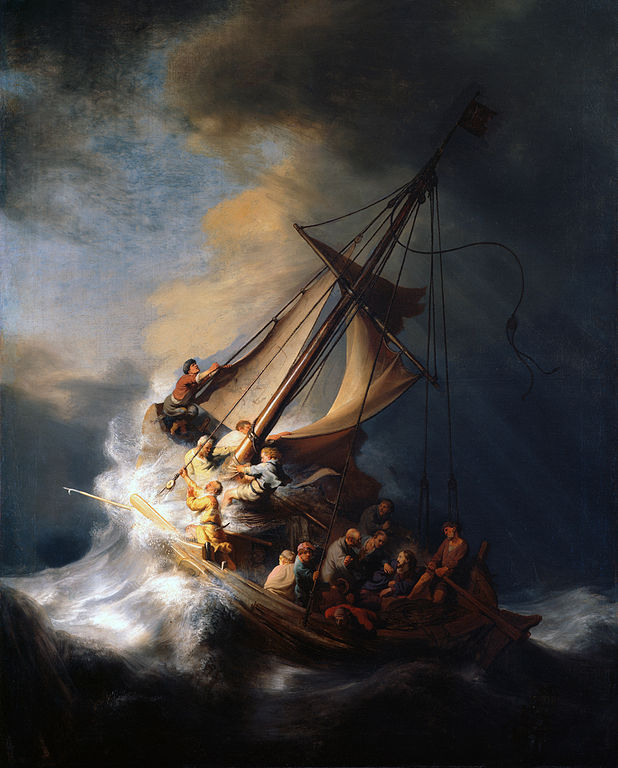
\includegraphics[width=0.4\textwidth]{figs/rembrandt_tempestade.png}
    \fonte{figrembrandt}
  \end{centering}
\end{wrapfigure}

\textbf{\emph{Rembrandt van Rijn}}, Holanda, 1606-69. É reconhecido
como o maior pintor da Holanda, dono de uma série de autorretratos que
contam de forma biográfica toda a sua vida.~\cite{van1999,
gombrich} Rembrandt usava a técnica do \textit{chiaroscuro} porém de
maneira diferente, como é possível ver em \textit{A Tempestade no Mar
da Galiléia} (figura~\ref{fig:rembrandt:tempestade}). Há grande
contraste, mas o fundo não está mergulhado em negro, ao contrário, o
céu complementa a composição, o mesmo pode se dizer do mar. Essa mesma
abordagem está presente nos retratos e outras cenas sagradas que
pintou.~\cite{van1997} Rembrandt
aproveita técnicas de seus antecessores, mas ao mesmo tempo, se
contrapõe a eles, adicionando nuances de seu próprio estilo.

\begin{wrapfigure}[12]{l}{0.5\textwidth}
  \vspace{-15pt}
%\begin{figure}[h!]
  \begin{centering}
    \caption{\emph{A Garota com Brinco de Pérola} (Johannes Vermeer), c. 1665}
    \label{fig:vermeer:perola}
    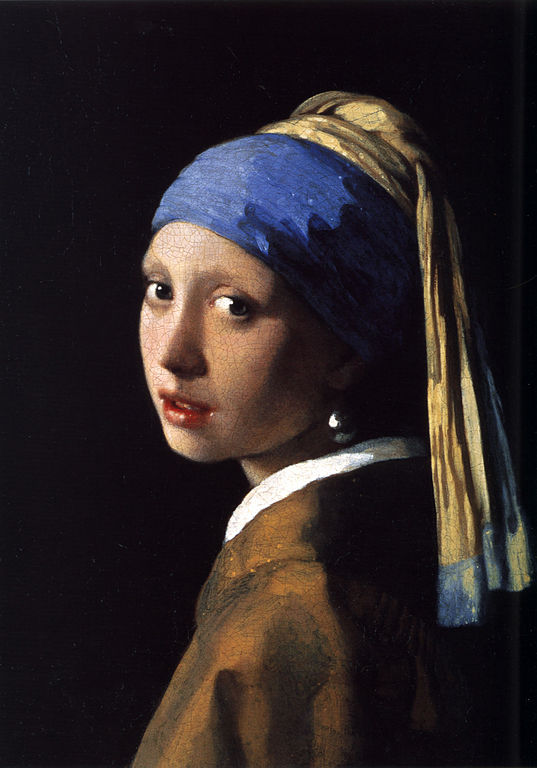
\includegraphics[scale=1.2]{figs/vermeer_perola.png}
    \fonte{figvermeer}
  \end{centering}
%\end{figure}
\end{wrapfigure}

\textbf{\emph{Johannes Vermeer}}, Holanda, 1632-1675. Uma das grandes realizações dos
pintores holandeses é a retratação da natureza-morta com incrível
detalhismo.~\cite{wadum} Vermeer é considerado o grande mestre deste
estilo, mas ao invés de objetos, incluía pessoas em sua
``natureza-morta''.~\cite{gombrich} Vermeer parece procurar a melhor
vestimenta, a melhor pose do modelo e a melhor posição para o ponto de
luz. Parece experimentar com os objetos da cena até encontrar o que
deseja. É interessante também perceber a diferença de sua pintura
comparada a dos outros pintores aqui discutidos: todas são feitas
praticamente no mesmo local --- sempre um cômodo doméstico --- e com
um número limitado de modelos, geralmente com a luz vindo de uma
janela.~\cite{wadum}  Em suas pinturas há, a exemplo de Velázquez,
uso extensivo do \textit{chiaroscuro} de Caravaggio, como em \textit{A
Garota com Brinco de Pérola}
(figura~\ref{fig:vermeer:perola}). Vermeer desconhecia a perspectiva
geométrica: a profundidade em seus quadros era obtida através do
reconhecido detalhismo deste pintor e outros holandeses.



\subsection{Arte Moderna}

\setlength{\epigraphwidth}{0.8\textwidth}
\epigraph{Cada época de uma civilização cria uma arte que lhe é própria e que
  jamais se verá renascer. Tentar revivificar os princípios artísticos de
  séculos passados só pode levar à produção de obras natimortas. Assim como é
  impossível fazer reviver em nós o espírito e as maneiras de sentir dos antigos
  gregos, também os esforços tentados para aplicar seus princípios [...] só
  levarão à criação de formas semelhantes às formas gregas. A obra assim
  produzida será sem alma para sempre.}{Wassily Kandinsky~\cite{kandinsky}}

De Vermeer à Van Gogh, passam-se por volta de 150 anos: o Rococó, o
Neoclassicismo, o Realismo, chegando aos movimentos da Arte
Moderna. Ao contrário do Barroco, a Arte Moderna parece não
compartilhar estéticas ou técnicas.~\cite{dempsey} Cada pintor aplica
ou cria novas formas de representar o que vê ou sente. Como dito por
Gombrich:~\cite{gombrich} ``[os pintores modernos] ansiavam por uma
arte que não consistisse de truques que poderiam ser aprendidos, por
um estilo que não é meramente um estilo, mas algo forte e poderoso
como a paixão humana''. Van Gogh procurou por essa arte através do uso
intenso de cores e aspecto caricato de suas pinturas.~\cite{hulsker}
Paul Gauguin buscou no ``primitivismo''~\cite{lovejoy} encontrar as
raízes da representação da natureza. Outros como Seurat~\cite{kemp}
usaram da observação de propriedades físicas da visão cromática para
pintar a natureza como uma coleção de pontos coloridos e dessa forma
acabou criando o pontilhismo. Os pintores modernos criam seu próprio
estilo de maneira individualista, sem a influência de seus
contemporâneos ou predecessores.~\cite{gombrich}

A Arte Moderna é representada nesse estudo pelos seguintes pintores,
que inclui representantes dos movimentos Pós-impressionista,
Expressionista, Cubista, Surrealista, Dada e Abstrato:

\begin{wrapfigure}[10]{r}{0.5\textwidth}
  \vspace{-15pt}
  \begin{centering}
    \caption{\emph{Quarto em Arles} (Vincent van Gogh), c. 1889}
    \label{fig:vangogh:quarto}
    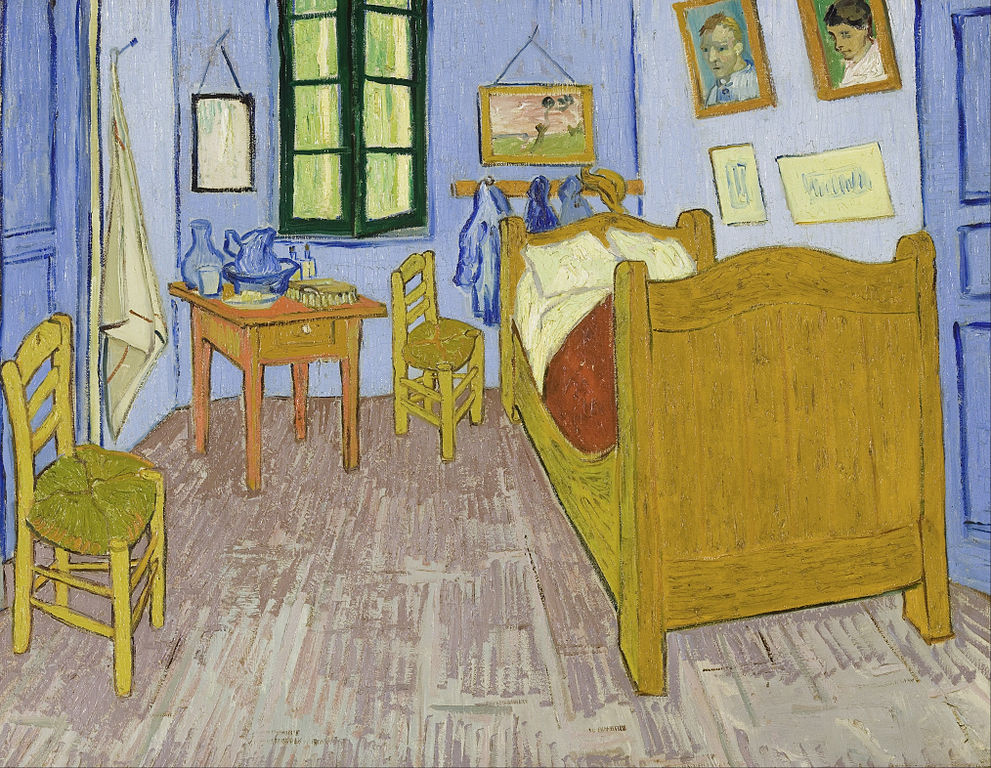
\includegraphics[width=0.5\textwidth]{figs/vangogh_quarto.png}
    \fonte{figvangogh}
  \end{centering}
\end{wrapfigure}

\textbf{\emph{Vincent van Gogh}}, Holanda, 1853-1890. Junto com
Cezánne e Gaugin, Van Gogh antecede o que veio a ser conhecido como
``Arte Moderna.''~\cite{gombrich} Cada pincelada de Van Gogh revela
sua sensação ao estar pintando, sua emoção; e garantem movimento à
composição. Não estava interessado em respeitar regras de perspectiva,
de composição, ou sombra.~\cite{hulsker} É possível perceber essa
oposição ao clássico em sua obra \textit{Quarto em Arles}
(figura~\ref{fig:vangogh:quarto}). Os móveis não apresentam
a perspectiva esperada, muito menos dimensões corretas. Não há sombra na
pintura. Propunha usar as cores de maneira franca, sem se render às
técnicas de sombreado. As pinceladas são todas aparentes, formam a
própria textura. Nada têm de parecido com as obras barrocas, ou mesmo
às impressionistas. Usava a distorção dos objetos para expressar o que
sentia. Vale complementar tal figura com as palavras do próprio Van
Gogh em uma de suas inúmeras cartas: ``Lamentavelmente, meu caríssimo
amigo, o público apenas verá nesse exagero uma caricatura --- mas o
que nos importa isso?''.~\cite{van1958} Mesmo sem perceber, acabara
por desempenhar um papel revolucionário para as artes, e se opõe assim
a todos os pintores conhecidos até então.

\textbf{\emph{Wassily Kandinsky}}, Rússia, 1866-1944. Possivelmente
inaugurou o que veio a ser conhecido como ``Arte Abstrata'' onde
nenhum objeto é reconhecível na pintura.~\cite{duchting} 

\begin{wrapfigure}[14]{l}{0.5\textwidth}
  \begin{centering}
    \caption{\emph{Em Branco} (Wassily Kandinsky), c. 1923}
    \label{fig:kandinsky:white}
    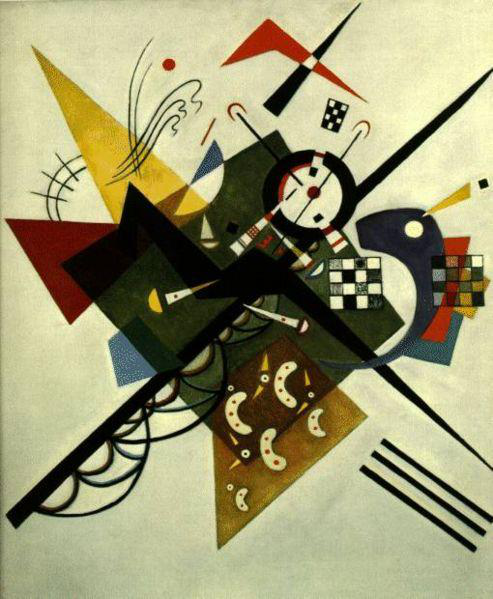
\includegraphics[width=0.5\textwidth]{figs/kandinsky_white.png}
    \fonte{figkandinsky}
  \end{centering}
\end{wrapfigure}

Suas pinturas
encontram ressonância com a música cromática (encontrada já em Bach em
seu ``Cravo Bem Temperado'', tornando-se elemento expressivo no fim do
período romântico, com Lizt, Mahler e Wagner, e acabando por
impulsionar o atonalismo da música serial dodecafônica, já no século
XX) no sentido do uso de toda a escala cromática em uma
composição.~\cite{gombrich} Kandinsky estava interessado no efeito perceptivo da cor pura, na
interpretação psicológica das cores.~\cite{ione} Assim, formas que
lembrassem objetos da natureza não eram necessárias, como visível na
figura~\ref{fig:kandinsky:white}. Esse uso das cores de maneira direta
e franca já tinha sido anunciado por Van Gogh, que negava o uso de
sombras para tornar as cores ainda mais aparentes e expressivas, algo
visto também em Kandinsky e Matisse.

\textbf{\emph{Henri Matisse}}, França, 1869-1954. Foi o mais famoso
pintor do grupo parisiense conhecido como \textit{Lez Fauves}, ou ``os
selvagens'', os Fauvistas.~\cite{elderfield,freeman} Tal grupo foi assim chamado pelo desprezo às formas encontradas na
natureza e pelo uso de cores ``violentas'' em suas
pinturas. Dedicou-se à ``simplificação decorativa'' ao estudar os
esquemas de cores de tapetes orientais e transpor estes esquemas para
seus quadros.~\cite{gombrich} Como visto na
figura~\ref{fig:matisse:red} há harmonia entre todos os elementos da
pintura, fazendo com que pareçam formar um único padrão, como em um
tapete. Até mesmo a paisagem vista da janela parece integrar-se com a
sala. Os desenhos do papel de parede são encontrados também na toalha
da mesa. 

\begin{wrapfigure}[10]{r}{0.5\textwidth}
  \begin{centering}
    \caption{\emph{A mesa de jantar: harmonia em vermelho} (Henri Matisse), c. 1908}
    \label{fig:matisse:red}
    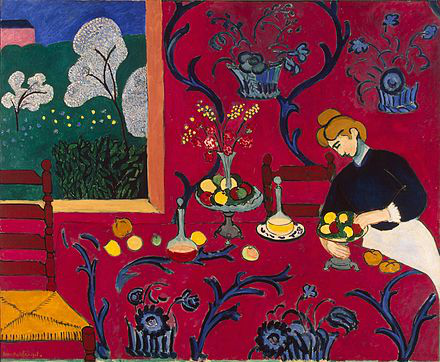
\includegraphics[width=0.5\textwidth]{figs/matisse_red.png}
    \fonte{figmatisse}
  \end{centering}
\end{wrapfigure}

Os contornos simples desses desenhos estão presentes também na
figura humana e em todos os utensílios da sala. Por esses motivos, o
pintor a chamou de ``harmonia em vermelho'', ressaltando a importância
da cor na obra.~\cite{matisse}


\textbf{\emph{Pablo Picasso}}, Espanha, 1881-1973. Estava interessado
no problema de representar uma imagem através de objetos simples, mas
sem perder suas características de solidez e
profundidade.~\cite{daix,gombrich} 

\begin{wrapfigure}[13]{r}{0.5\textwidth}
  \begin{centering}
    \caption{\emph{Violino} (Pablo Picasso), c. 1911-12}
    \label{fig:picasso:violino}
    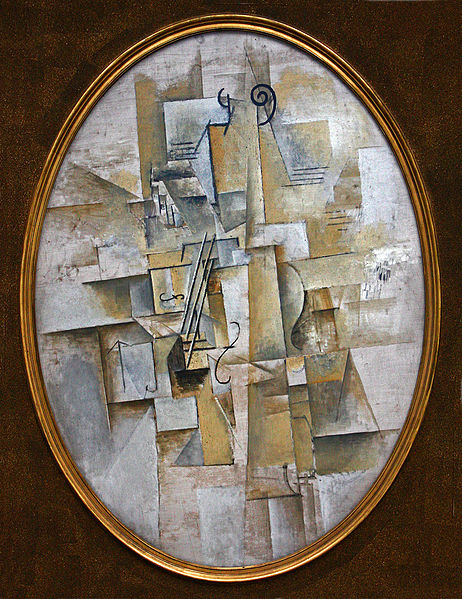
\includegraphics[width=0.4\textwidth]{figs/picasso_violino.png}
    \fonte{figpicasso}
  \end{centering}
\end{wrapfigure}

Influenciado por Cézanne,~\cite{rishel} emprega de forma literal seu
conselho de observar a natureza como um conjunto de esferas, cones e
cilindros. Procura então representar o que vê como um complexo de
peças uniformes, cada uma representando uma faceta do que está sendo
retratado. Cria assim o movimento cubista.~\cite{barr,golding} Essa
colagem geométrica é vista em \emph{Violino}
(figura~\ref{fig:picasso:violino}). De certa forma, relembra os
desenhos ``primitivos'' que retratam o objeto a partir do ponto de
vista que mais lhe representa. As formas do violino repetem-se por
toda a pintura: como as curvas da \textit{voluta}, dos \textit{efes} e
do \textit{corpo}. O mesmo grupo de 4 cordas aparece diversas vezes,
como que querendo representá-las de vários pontos de
vista. Essa \textit{colagem de pontos de vista} remete ao que acontece
quando tenta-se resgatar um objeto da memória. Quando imagina-se um
violino, sua forma é exagerada. Não se imagina um violino específico,
mas um conjunto de detalhes de todos os violinos que já foram vistos
algum dia. Embora seja uma colagem de formas desconexas, a pintura
aparenta organização, como se seu todo desse sentido ao objeto já
conhecido.~\cite{gombrich}

\begin{wrapfigure}[10]{r}{0.5\textwidth}
  \vspace{-15pt}
  \begin{centering}
      \caption{\emph{O Campo Cultivado} (Joan Miró), c. 1923-24}
     \label{fig:miro:campo}
    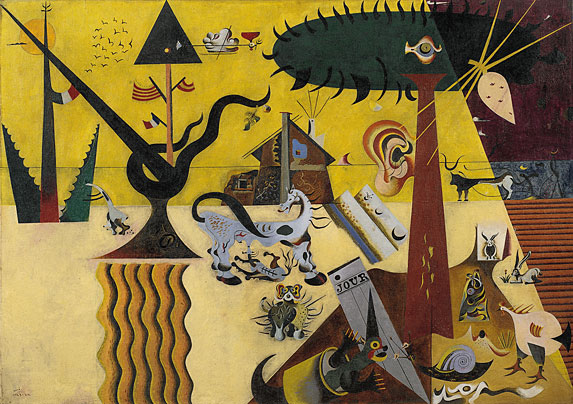
\includegraphics[width=0.5\textwidth]{figs/miro_campo.png}
    \fonte{figmiro}
  \end{centering}
\end{wrapfigure}

\textbf{\emph{Joan Miró}}, Espanha, 1893-1983. Inicialmente teve sua fase
fauvista mas tornou-se reconhecidamente um surrealista. Miró foi um
dos primeiros artistas a desenvolver a ``escrita automática'', uma
técnica onde o artista deixa sua mão mover-se livremente pelo papel,
transferindo o desenho, em seguida, para a tela.~\cite{montagu} Queria
com isso se desfazer das técnicas de pintura já
estabelecidas. Utilizou também um dicionário de símbolos abstratos
para representar objetos reais (e.g.\ um triângulo para a cabeça,
linhas curvas para um bigode) como é visto na
figura~\ref{fig:miro:campo}, onde sua obra acaba por se tornar uma
colagem destes símbolos.~\cite{stich}

\textbf{\emph{Jackson Pollock}}, Estados Unidos, 1912-1956. Abandonou
as imagens fantásticas do Surrealismo e os métodos convencionais de
pintura. Pintava com as telas jogadas no chão, gotejando ou
arremessando suas tintas, em pé, sobre as telas. O complexo de linhas
(visto na figura~\ref{fig:pollock:ritmo}) reflete o desejo de
simplificação dos artistas modernos assim como sua busca por uma
``pintura pura.''~\cite{gombrich}

\begin{figure}[h!]
  \begin{center}
  \caption{\emph{Ritmo de Outono} (Jackson Pollock), c. 1950}
  \label{fig:pollock:ritmo}
    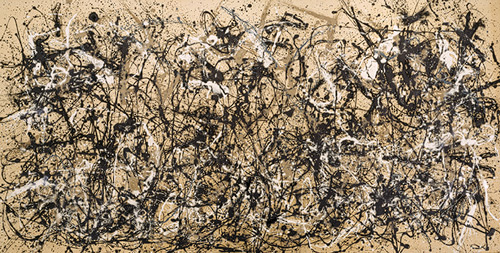
\includegraphics[scale=1.2]{figs/pollock_ritmo.png}
    \fonte{figpo}
  \end{center}
\end{figure}

Pollock trilhou essa busca através do que ficou conhecido como
``pintura de ação'': uma pintura não premeditada, criada por impulso
espontâneo. Isso é afirmado pelo próprio pintor: ``Não trabalho a
partir de desenhos ou esboços em cores. Minha pintura é direta. [...]
O método de pintar é o resultado natural de uma necessidade. Quero
expressar meus sentimentos, e não ilustrá-los. A técnica é apenas um
meio de chegar a uma declaração. Quando estou pintando, tenho uma
ideia geral do que estou fazendo. Posso controlar o fluxo da pintura:
não há acidentes, assim como não há começo nem fim. Eu não tenho medo
de fazer mudanças, de destruir a imagem, porquê a pintura tem vida
própria. Eu tento deixar ela viver.''.~\cite{pollock}

\subsection{Sumário de características do período Barroco e de movimentos da Arte Moderna}
\label{subsec:sumario}

Dadas as características presentes nas obras dos pintores escolhidos,
pode-se sumarizar um conjunto de afirmações que serão confrontadas no
Capítulo~\ref{chap:resultados} de resultados:

\begin{itemize}
\item Os pintores da Arte Moderna são caracterizados por sua
  independência em estilo: há pouca similaridade entre suas obras e de
  suas obras com àquelas do período Barroco. Já os pintores do período
  Barroco apresentam semelhanças, por compartilharem estilos
  tradicionais. Embora hajam também oposições, como entre Poussin e
  Caravaggio.

\item Há uma diferença cronológica considerável entre o Barroco
  e os movimentos da Arte Moderna, assim como diferenças estéticas
  marcantes entre estes dois períodos;

\item Pollock apresenta pinturas que diferem de todos os outros
  pintores escolhidos. Suas pinturas chegam a sugerir aleatoriedade,
  contrastando até mesmo com pintores também surrealistas como Miró e
  afastando-se por completo dos artistas barrocos;

\item Velázquez e Vermeer se assemelham com Caravaggio pois ambos
  utilizavam \textit{chiaroscuro}. Velázquez chegou a estudar as
  pinturas de Caravaggio e a semelhança de suas obras é notável;

\item Caravaggio é expoente no uso da técnica do
  \textit{chiaroscuro}, apresentando pinturas com predominância de
  cores escuras. Portanto há grande diferença de contraste entre suas
  pinturas e àquelas mais modernas, sendo estas mais claras;

\item Poussin se opõe à Caravaggio: ele não deseja retratar a verdade, 
mas sim o belo. A técnica do \textit{chiaroscuro} não é encontrada em
Poussin, suas pinturas são mais claras, lembrando as pinturas de
Carracci, Reni ou mesmo Rafael.

\item O Barroco tem como objetivo principal retratar emoções,
  movimento. É possível perceber que pinturas como as de Caravaggio
  tinham o intuito de chocar, principalmente por se tratarem de
  retratações sagradas.
\end{itemize}

A tabela~\ref{tab:caracarts} resume de maneira pontual as
características que marcam as obras da grande maioria dos pintores do
período Barroco, assim como aquelas que fazem parte das obras de cada
pintor moderno:

\begin{table}[h]

  \begin{center}
\caption{\label{tab:caracarts} Sumário de características do período Barroco e de cada artista dos movimentos da Arte Moderna estudados.}
 \resizebox{\textwidth}{!}{%

\begin{tabular}{|l|ll|}
\hline \hline
\textbf{Barroco}                                                                                                                   & \multicolumn{2}{l|}{\textbf{Arte Moderna}}                                                                                                                               \\ \hline
\multirow{6}{*}{\begin{tabular}[c]{@{}l@{}}Contraste (e.g. claro-escuro); \\ emoção ao invés da razão; movimento; \\ dramaticidade; sensualidade; \\ beleza; fantasia; \\ a verdade; o sagrado\end{tabular}} & Van Gogh  & \begin{tabular}[c]{@{}l@{}}Sensação; movimento; textura; cores; \\ uso da perspectiva e profundidade de uma \\ nova maneira; distorção\end{tabular} \\ \cline{2-3} 
                                                                                                                          & Kandinsky & \begin{tabular}[c]{@{}l@{}}Abstrato; cromatismo; \\ interpretação psicológica; \\ formas geométricas, puras\end{tabular}                            \\ \cline{2-3} 
                                                                                                                          & Matisse   & \begin{tabular}[c]{@{}l@{}}Cores ``violentas''; desprezo às formas \\ naturais; decoração; simplicidade\end{tabular}                                \\ \cline{2-3} 
                                                                                                                          & Picasso   & \begin{tabular}[c]{@{}l@{}}Solidez; simplicidade; formas geométricas; \\ colagem de várias perspectivas\end{tabular}                                \\ \cline{2-3} 
                                                                                                                          & Miró      & \begin{tabular}[c]{@{}l@{}}Surreal; automatismo; símbolos e seus \\ significados; negação das técnicas de \\ pintura existentes\end{tabular}        \\ \cline{2-3} 
                                                                                                                          & Pollock   & Abstrato; pintura de ação, pura, espontânea                                                                                                         \\ \hline \hline
\end{tabular}
}
\fonteminha
\end{center}

\end{table}

\section{Conceitos básicos em Filosofia}
\label{sec:fund:filosofia}

\textit{Dialética}, \textit{oposição} e \textit{inovação} são conceitos essenciais nas discussões
filosóficas. A \textit{dialética} é vista como método filosófico para
argumentação, central na Filosofia ocidental e
oriental.~\cite{deleuze,pinto,van} Para Platão, o método dialético era
o próprio método científico, onde se investiga racionalmente um
determinado conceito.~\cite{pinto} Cada conceito deve ser confrontado
com outras teorias e situações para se chegar a uma nova teoria. Hegel
sumariza o método dialético~\cite{van} em três momentos bem definidos:
a \textit{tese}, um argumento ou ideia tomado como verdadeiro;
a \textit{antítese}, a contradição ou negação da tese; e
a \textit{síntese}, o resultado do confronto da tese com a antítese. A
solução dialética --- a síntese --- é uma nova ideia que busca pelo
equilíbrio entre tese e antítese, ilustrado na
figura~\ref{fig:conceitos}. 

Como a tradução literal sugere, ``o
caminho entre as ideias'' é o diálogo entre ideias que leva a outras
ideias, ou teorias. Zenão de Eleia, Aristóteles, Platão e Sócrates
foram pioneiros em seu uso. A dialética também está presente
no \textit{método dialético} de Hegel e na \textit{dialética
materialista} de Marx, que propõe utilizar a dialética como um método
propriamente científico, aplicando-a diretamente à
realidade.~\cite{dialectics}

\begin{figure}[ht!]
\begin{center}
\caption{\textit{a)} \textit{Dialética}: um argumento chamado \textit{tese}, até então
  tomado como verdade, é confrontado por um argumento oposto,
  chamado \textit{antítese}. O resultado do confronto destas duas
  ideias é a \textit{síntese}, que poderá gerar uma nova ideia ou
  argumento. A linha pontilhada simboliza a \textit{síntese ótima} entre tese e antítese. Portanto, um argumento que se aproxime dessa linha terá alta dialética; \textit{b)} \textit{Oposição}: é um argumento que se opõe
  a um argumento original, afasta-se da linha pontilhada de referência. Esta linha de referência é necessária, pois não trata-se apenas de um argumento anterior, mas um conjunto deles. Ela simboliza, no diagrama, um \textit{estado médio} considerando todos os argumentos originais que antecedem o argumento de posição. Assim, um argumento que se afasta da linha de referência estaria se opondo a tal argumento, e vice-versa; \textit{c)} \textit{Inovação}: um movimento
  de inovação é aquele que se afasta do argumento original, inovando: toma uma nova direção quando comparada à linha pontilhada de referência. Esta linha de referência também demarca o estado médio dos argumentos originais. Portanto, argumentos que tomam uma direção diferente da referência estariam inovando. Nota-se também que há uma ordem temporal dos argumentos, representada pelos números. Para a dialética: primeiro há a tese, em seguida a antítese e, por fim, a síntese. Para a oposição, há o argumento original seguido do argumento de oposição. Para a inovação, há o argumento original seguido do argumento de inovação.}
\label{fig:conceitos}

\vspace{30pt}

\begin{tikzpicture}[scale=1.]
  % Dialética
  \node[draw] (Tese) at (0,0) {1: Tese};
  \node[draw,fill=black,text=white] (Antitese) at (2.3,0) {2: Antítese};
  \node[draw,fill=gray,text=white] (Sintese) at (2.1,2) {3: Síntese};
  
  \draw[dotted,draw=black] (1,-3) to (1,3);
  \draw[->,draw=blue] (Tese) to (Antitese);
  \draw[->,draw=blue] (Antitese) to (Sintese);
  %\draw[->,draw=blue] (Sintese) to[in=180,out=180] (Tese);
  
  \node at (1.0, -5.0) {\textit{a) Dialética}};
  
  % Oposição  
  \node[draw] (ArgumentoA) at (5,-1.5) {1: Argumento};
  \node[draw,fill=black,text=white] (ArgumentoB) at (8.0,-1.5) {2: Oposição};
  
  \draw[dotted,draw=black] (6.6,-4.5) to (6.6,1.5);
  \draw[->,draw=blue] (ArgumentoA) to (ArgumentoB);
  
  \node at (6., -5.0) {\textit{b) Oposição}};
  
  % Inovação
  \draw[dotted,draw=black] (9,0) to (14,0);
  %\node at (6., -1.0) {\textit{b) Oposição}};

  \node[draw] (ArgumentoA) at (11,0) {1: Argumento};
  %\node[draw,fill=black,text=white] (ArgumentoB) at (12.8,0) {Oposição};
  \node[draw,fill=yellow] (ArgumentoC) at (12,2) {2: Inovação};
  
  %\draw node[vertex] (Juncao) at (11.5,0) {};
  
  %\draw[-] (ArgumentoA) to (Juncao);
  %\draw[->] (Juncao) to (ArgumentoB);
  \draw[->,draw=blue] (ArgumentoA) to (ArgumentoC);
  
  \node at (11.5, -5.0) {\textit{c) Inovação}};

\end{tikzpicture}
\vspace{30pt}
\fonteminha

\end{center}
\end{figure}

A \textit{oposição} de ideias está intimamente relacionada à
dialética. Frequentemente, há grande oposição entre a tese e a
antítese (figura~\ref{fig:conceitos}, detalhe \textit{b}), sendo
ideias essencialmente contraditórias. A \textit{inovação}, por sua
vez, relaciona-se com a oposição: uma ideia não necessariamente estará
destinada a opor uma outra ideia, pois não participa apenas de um
``jogo de oposição''. Uma ideia pode também ``buscar'' um movimento
novo, alternativo. Desta forma, estará inovando, contrastando com a oposição, indo em uma nova direção
(figura~\ref{fig:conceitos}, detalhe \textit{c}). É importante notar que há uma ordem temporal nos argumentos, simbolizados na figura por números. No caso da dialética, há primeiramente a tese, seguida da antítese e, por fim, a síntese. Portanto, compreende três estados temporais. O mesmo ocorre para a oposição e inovação, porém compreendendo apenas dois estados no tempo.

Uma proposta de quantificar os conceitos básicos de dialética,
oposição e inovação foi iniciado em um estudo aplicado à Filosofia e
Música.~\cite{vieira} A partir de uma matriz de atributos que descreve
pesos (ou notas) dadas em conjunto pelos autores à certas
características de filósofos e músicos, tem-se um espaço vetorial onde
os conceitos são quantificados. Esse estudo está sendo aqui expandido.
As mesmas medidas são aplicadas, mas não mais à notas que poderiam ser
julgadas como subjetivas --- já que atribuídas por humanos. Ao invés
disso, as notas são substituídas por vetores de atributos, extraídos
através do processamento de imagens (discutido nas
seções~\ref{sec:fund:imagens} e~\ref{sec:medidas}).

\section{Momentos estatísticos}
\label{sec:momentos}

Alguns momentos de distribuição da Estatística Descritiva ou Teoria de
Probabilidades são utilizados durante todo este estudo e cabe aqui uma
rápida revisão. Primeiramente, os momentos estatísticos centrais,
úteis quando se observa uma tendência central nas variáveis aleatórias
--- ou seja, quando os dados tendem a agruparem-se em torno de um
valor específico. Considerando a variável aleatória $X$,
sua \textit{média} é definida como~\cite{recipes}

\begin{equation}
\text{média}(X) = m_x=\mu_x=\overline{x}=\frac{\sum_{i=1}^{n}X_i}{n}
\end{equation}

\noindent e estima o valor central, em volta do qual os valores $X_i$ agrupam-se. Um outro momento usado para estimar a centralidade é a \textit{mediana}, definida como

\begin{equation}
\text{mediana}(X) = \text{\~{x}} =\mu_{1/2}= \begin{cases}
                               X_{(n+1)/2} & n \,\, \text{ímpar} \\
                               \text{média}(X_{n/2}, X_{n/2+1}) & n \,\, \text{par}
                               \end{cases} \,\,\,\,\, (\text{estando $X$ ordenado}).
\end{equation}

Após ter-se definido o valor central, pode-se estimar o
espalhamento ou quanto os valores variam em torno do valor
central. A \textit{variância} é geralmente utilizada para este fim:

\begin{equation}
\text{variância}(X)=var_x=\sigma^2_x=s^2_x=\frac{\sum_{i=1}^{n}(X_i-\mu_x)^2}{n-1}
\end{equation}

\noindent assim como o \textit{desvio padrão}, que corresponde à raiz quadrada da variância:

\begin{equation}
\text{desvio\;padrão}(X)=std(X)=\sigma_x=s_x=\sqrt{\frac{\sum_{i=1}^{n}(X_i-\mu_x)^2}{n}}.
\end{equation}

Ao se considerar duas variáveis aleatórias $X$ e $Y$, pode-se estender
o cálculo da variância para estimar-se o grau de interdependência
entre as duas variáveis aleatórias:

\begin{equation}
\text{covariância}(X,Y)=cov(X,Y)=c_{X,Y}=\frac{\sum_{i=1}^{n}(X_i-\mu_x)(Y_i-\mu_y) }{n}
\end{equation}

É interessante notar que variáveis independentes terão covariância
igual a zero.

\section{Processamento e análise de imagens digitais}
\label{sec:fund:imagens}

O processamento e análise de imagens digitais compreende operações para
adquirir, manipular e representar imagens digitais em um sistema
computacional.~\cite{gonzalez} Este processamento envolve uma série de
etapas canônicas~\cite{luciano} e a figura~\ref{fig:etapas-pdi}
apresenta as etapas utilizadas neste estudo. Estas operações são
necessárias para extrair os vetores de características de uma
imagem. Na presente seção são discutidas as etapas utilizadas neste
estudo.

\begin{figure}[ht!]
\begin{center}
 \caption{Etapas
      canônicas utilizadas neste estudo para o processamento de
      imagens.}  
\label{fig:etapas-pdi}
        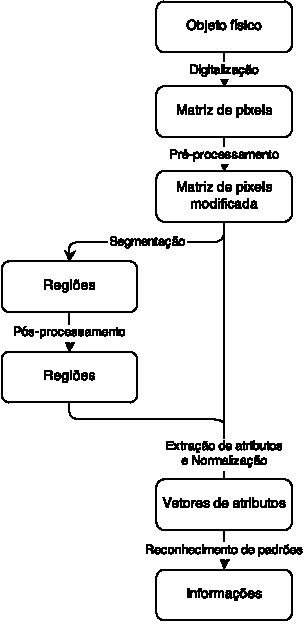
\includegraphics[scale=1.]{figs/etapas_pdi} 
\fonteminha
\end{center}
\end{figure}

Cada imagem, após ser digitalizada, é representada como uma matriz de
valores onde cada elemento armazena a intensidade luminosa de uma
região amostrada da imagem analógica. Uma imagem colorida $I$
representada no formato digital conhecido como RGB (as bandas de cores
primárias vermelha, verde e azul) é definida como a matriz $I$ de
valores discretos $I_{(x,y)}$ com dimensão $N_x \times N_y \times
N_z$. Os valores $N_x$ e $N_y$ são, respectivamente, a quantidade
de \textit{pixels} das linhas e colunas de $I$, e $N_z$ determina a
quantidade de bandas de cores da imagem --- e.g.\ para uma imagem RGB
de $800 \times 800$ \textit{pixels}, a dimensão de sua representação
matricial é $800 \times 800 \times 3$. Cada elemento $I_{(x,y)}$ da
matriz corresponde a uma \emph{tripla} $(R, G, B)$ de valores inteiros
compreendidos entre 0 e 255, onde 0 é a intensidade de cor mais
escura, e 255 a mais clara. A combinação destas três intensidades
resulta na cor do \textit{pixel}.

As imagens também podem ser representadas em escala de cinza (ou
monocromática), por uma matriz $I$ com dimensão $N_x \times N_y \times
N_z$, com $N_z = 1$, onde cada \textit{pixel} $I_{(x,y)}$ é descrito por um único valor de
intensidade. Nota-se que cada banda de cor de uma imagem RGB
corresponde a uma imagem monocromática.

Alguns algoritmos utilizam a imagem representada com apenas dois
valores: preto e branco. Por exemplo, em uma imagem segmentada, os
elementos conexos podem ser representados com a cor branca e fundo
preto. A matriz para esta representação binária é definida como $I$
tendo dimensão $N_x \times N_y$. Cada um de seus elementos $I_{(x,y)}$
pode assumir apenas dois valores, 0 ou 255. Convenciona-se usar também
os valores 0 ou 1, dado o aspecto binário da matriz e para facilitar a
aplicação de operações lógicas sobre elas.~\cite{gonzalez}

Uma imagem $I$ é também definida como uma função $f(x,y)$ que mapeia
os índices matriciais $(x,y)$ de um \textit{pixel} em seu valor $v$ de
intensidade. Sendo $S_x = \{0, 1, ..., N_x - 1\}$ e $S_y = \{0, 1,
..., N_y - 1\}$ o domínio espacial da imagem e $S_v = \{0, 1, ...,
255\}$ o domínio de $v$, tem-se a função

\begin{equation}
  f : S_x \times S_y \to S_v
\end{equation}

\noindent para imagens binárias o domínio será $S_v = \{0, 255\}$ ou $S_v = \{0,
1\}$, representando assim os possíveis níveis de intensidade da
imagem.~\cite{gonzalez}

\subsection{Vizinhança e operadores espaciais}

As relações locais entre \textit{pixels} de uma imagem são realizadas
entre um determinado \textit{pixel} $I_{(x,y)}$ e seus
vizinhos. Algoritmos para pré-processamento (e.g.\ equalização por
histograma, ou filtro de medianas) e até mesmo para extração de
características (e.g.\ algoritmo de curvatura ou cálculo de entropia
local) utilizam esta relação.~\cite{gonzalez} Os vizinhos de
um \textit{pixel} $I_{(x,y)}$ são os $N_V$ \textit{pixels} $V_i$ que o
circundam, e costuma-se chamar este conjunto
de \emph{vizinhança}-$N_V$ com $0 \leq i \leq N_V$. Duas vizinhanças
são comuns: a vizinhança-4 e vizinhança-8, ilustradas na figura~\ref{fig:vizinhanca}. 

\begin{figure}[ht!]
\begin{center}
      \caption{Coordenadas das vizinhanças-$4$ e $8$ para um dado \textit{pixel}
        $I_{(x,y)}$ qualquer.}
        \label{fig:vizinhanca}

\begin{tikzpicture}[thick]
\draw (0,0) grid (3,3);
\node at (1.5,1.5) {$I_{(x,y)}$};

\node at (2.5,1.5) {$V_0$};
\node at (1.5,2.5) {$V_1$};
\node at (0.5,1.5) {$V_2$};
\node at (1.5,0.5) {$V_3$};

\draw (1.5,0) node[below] {vizinhança-$4$};
\end{tikzpicture}
\hspace{2pc}
\begin{tikzpicture}[thick]
\draw (0,0) grid (3,3);
\node at (1.5,1.5) {$I_{(x,y)}$};

\node at (2.5,1.5) {$V_0$};
\node at (2.5,2.5) {$V_1$};
\node at (1.5,2.5) {$V_2$};
\node at (0.5,2.5) {$V_3$};
\node at (0.5,1.5) {$V_4$};
\node at (0.5,0.5) {$V_5$};
\node at (1.5,0.5) {$V_6$};
\node at (2.5,0.5) {$V_7$};

\draw (1.5,0) node[below] {vizinhança-$8$};
\end{tikzpicture}
\fonteminha
\end{center}
\end{figure}

Dado um \textit{pixel} $I_{(x,y)}$,
sua vizinhança-4 corresponde aos seguintes conjuntos:

\begin{eqnarray}
  V_0 & = & (x, y+1) \\
  V_1 & = & (x-1, y) \\
  V_2 & = & (x, y-1) \\
  V_3 & = & (x+1, y)
\end{eqnarray}

\noindent e sua vizinhança-8 é definida por:

\begin{eqnarray}
  V_0 & = & (x, y+1) \\
  V_1 & = & (x-1, y+1) \\
  V_2 & = & (x-1, y) \\
  V_3 & = & (x-1, y-1) \\
  V_4 & = & (x, y-1) \\
  V_5 & = & (x+1, y-1) \\
  V_6 & = & (x+1, y) \\
  V_7 & = & (x+1, y+1)
\end{eqnarray}

A partir da definição de vizinhança, pode-se definir uma função de
processamento no domínio espacial da imagem como

\begin{equation}
  g(x,y) = T[f(x,y)]
  \label{eq:fproc}
\end{equation}

\noindent sendo $f(x,y)$ a imagem de entrada, $g(x,y)$ a imagem
processada e $T$ um operador de $f$ definido sobre uma
vizinhança-$N_V$ do ponto $(x,y)$. Este processo consiste em mover o
centro da vizinhança-$N_V$ de \textit{pixel} a \textit{pixel} e aplicar o operador $T$
aos \textit{pixels} da vizinhança, obtendo-se o valor de $g(x,y)$ para cada
posição. Isso corresponde a alterar os valores $f(x,y)$ pelo valor
obtido ao aplicar $T$ à sua vizinhança. Apesar de ser possível
utilizar várias formas para a vizinhança (e.g.\ círculos ou elipses),
as formas quadradas são mais comuns por serem de fácil
implementação.~\cite{gonzalez}

Pode-se também aplicar o operador $T$ diretamente em um \textit{pixel}
$(x,y)$. Para isso utiliza-se uma janela de dimensões $1 \times 1$
centrada no próprio \textit{pixel}. Assim, $g$ depende apenas do valor de $f$
em um único ponto. Neste caso, $T$ é definido como uma função de
transformação de intensidade:

\begin{equation}
  s = T(r)
\end{equation} 

\noindent onde $s$ e $r$ representam a intensidade de $g$ e $f$ em qualquer \textit{pixel} $(x,y)$. 
Ou seja, os níveis de intensidade da imagem processada dependerão da
operação definida em $T$. A equalização de uma imagem de entrada a
partir de um operador $T$ baseado no histograma de tons de cinza da
imagem é um exemplo de aplicação, discutido em detalhes na
subseção~\ref{sec:preproc}.

\subsection{Pré-processamento}
\label{sec:preproc}

A etapa de pré-processamento tem como objetivo melhorar certos
aspectos de uma imagem digital. É possível então corrigir falhas
ocorridas durante a aquisição da imagem ou realçar certos detalhes de
interesse. Caso não aplicado o pré-processamento, o resultado de um
posterior processamento pode ser comprometido, já que as
características naturais da imagem podem ter sido
degradadas.~\cite{luciano,gonzalez}

As operações de pré-processamento podem ser realizadas no domínio real
e das frequências. No domínio real, os próprios elementos da matriz
$I$ são alterados diretamente. Já o domínio das frequências envolve a
transformada de Fourier da matriz para manipular bandas de valores,
necessitando da transformada inversa para levar a matriz ao espaço
real novamente.

Uma operação recorrente de pré-processamento no domínio real, por ser
computacionalmente barata e eficiente, é a \emph{equalização por
  histograma}. O objetivo é ajustar o nível de contraste da imagem
baseando-se em seu histograma de valores. O histograma de uma imagem em escala de cinza
$I$ é dado pela função

\begin{equation}
\text{hist}(I) = p(R_k) = \frac{N_k}{N_I}
\end{equation}

\noindent onde $R_k$ é um nível de cinza $k$ específico, com $k \in \{0, 1, ...,
255\}$, $N_k$ é a quantidade de
\textit{pixels} da imagem $I$ que possuem nível de cinza $k$ e $N_I$ é a quantidade total de \textit{pixels} da imagem $I$. Ou seja,
$p(R_k)$ corresponde à probabilidade de ocorrência de um nível de
cinza $R_k$ na imagem. O gráfico de $p(R_k)$ é denominado
\emph{histograma}. Essa informação é interessante quando se deseja
realçar o contraste da imagem, visto que pode-se mensurar a quantidade
de \textit{pixels} em regiões mais claras, mais escuras e com níveis de cinza
medianos. Assim, pode-se definir uma operação $T$ (eq.~\ref{eq:fproc}) que equalize os
níveis de cinza $R_k$ de $f$, gerando uma imagem equalizada $g$ de $N_g$ \textit{pixels}:

\begin{equation}
s = T(R_k) = \sum_{j=0}^k \frac{N_j}{N_g} = \sum_{j=0}^k p(R_j)
\end{equation}

\noindent à essa operação $T$ se dá o nome de \emph{equalização de
  histograma} ou \emph{linearização de histograma}.~\cite{gonzalez} Ao
se mapear os níveis de cinza $R_k$ de $f$ nos níveis $s$ de $g$,
tem-se a imagem equalizada em contraste.

Após equalizar os níveis de contraste da imagem, é comum suavizá-la e
remover ruído através de filtros, como por exemplo, o filtro de
mediana. Esse efeito de suavização e remoção de ruídos ocorre pois
cada \textit{pixel} terá como seu valor a mediana de seus
vizinhos. Assim, quanto maior o tamanho da vizinhança, maior a
suavização em relação à imagem. O filtro de média também pode ser
utilizado. Porém, o filtro de mediana preserva detalhes de bordas que
são borrados pelo filtro de média.~\cite{gonzalez} Portanto o uso do
filtro de mediana é mais interessante para a análise de pinturas, já
que detalhes de formas são características que devem ser extraídas. O
que se quer é a eliminação de ruído sem borrar detalhes de borda.

Para implementar o filtro por mediana, troca-se o valor do nível de
cinza $R_k$ em $f$ pela mediana dos níveis de cinza da
vizinhança-$N_V$ desse \textit{pixel}. Essa operação
(eq.~\ref{eq:fproc}) pode ser definida como

\begin{equation}
  T[f(x,y)] = \text{mediana}(V_N(f(x,y)))
\end{equation}

\noindent onde $V_N(f(x,y))$ é o conjunto de \textit{pixels} na
vizinhança-$N_V$ com centro em $(x,y)$ na imagem $f$.

\subsection{Segmentação}
\label{sec:slic}

Embora a visão humana seja capaz de distinguir formas com relativa
precisão, é preciso aplicar um procedimento conhecido
como \emph{segmentação} para identificar formas da imagem em um
sistema computacional. Assim, o processo de segmentação tem como
objetivo particionar uma imagem em múltiplos segmentos que são na
realidade grupos de \textit{pixels}.

Há um grande número de algoritmos de segmentação, sendo uma área de
pesquisa rica e em constante desenvolvimento. Portanto, não há como
esgotar todo o conjunto de algoritmos existentes em via de testá-los
para a segmentação das pinturas. Uma prática comum é selecionar um
grupo de algoritmos e aplicá-los exaustivamente ao conjunto de imagens
e, de maneira experimental, escolher o algoritmo que mais contribui
para a segmentação pretendida. O algoritmo SLIC (\textit{Simple Linear
Iterative Clustering})~\cite{slic} é baseado em
\textit{superpixels} e aplicado em matrizes coloridas de imagens. Portanto,
para pinturas coloridas, seu uso é incentivado e demonstrou
segmentação esperada --- como pode ser visto na
seção~\ref{sec:analiseimagens}.

Algoritmos baseados em \textit{superpixels} como o SLIC agrupam \textit{pixels} em
regiões que tenham maior significado do que a simples malha de
\textit{pixels}. Essas regiões mais significativas são chamadas \textit{superpixels}. O
algoritmo SLIC agrupa os \textit{pixels} em \textit{superpixels}
através de uma adaptação do algoritmo de
clusterização \emph{k-means}. Apesar de ser uma ideia simples, se
mostra comparável aos algoritmos de \textit{superpixel} considerados
``estado da arte'' atualmente, chegando a superá-los para a
segmentação.~\cite{slic}

O algoritmo~\ref{algo:slic} lista os passos do procedimento
SLIC. Primeiramente, uma imagem RGB $I$ precisa ter seus elementos
convertidos para o padrão CIE 1976 $L*$ $a*$ $b*$ (ou simplesmente
CIELAB),~\cite{cielab1} que representa uma determinada cor em função
de um espaço definido pela base $(L*, a*, b*)$, ilustrado na
figura~\ref{fig:cielab}. $L*$ determina a quantidade de luminosidade
da cor enquanto o eixo $a*$ determina a matiz entre verde e vermelho,
e $b*$ a matiz entre azul e amarelo. A conversão do formato RGB para
CIELAB é discutida em detalhes por~\citeauthor{cielab2}.

\begin{figure}[ht!]
\begin{center}
    \caption{Espaço de cor CIELAB. Uma cor qualquer é representada como um ponto
    no espaço $(L*, a*, b*)$.}
  \label{fig:cielab}

  \begin{tikzpicture}
    % b* shade
    \path[draw, shade, left color=blue, right color=yellow, opacity=.6] 
    (0,0,0) node[below] {$-b*$} -- (5,2.0,0) node[below] {$+b*$} -- (5, 2.5, 0)
    -- (0, 0.5, 0) -- cycle;

    % a* shade
    \path[draw, shade, left color=green, right color=red, opacity=.6] 
    (0, 2.0, 0) node[below] {$-a*$} -- (5, 0, 0) node[below] {$+a*$} 
    -- (5, .5, 0) -- (0, 2.5, 0) -- cycle;
    
    % L* shade
    \path[draw, shade, top color=white, bottom color=black, opacity=.6] 
    (2.65, -1.85, 0) node[right] {$L* = 0$} -- (2.65, 4.45, 0) node[right] {$L*=100$}
    -- (2.35, 4.3, 0)  -- (2.35, -2., 0) -- cycle;

    % b*-axis
    \draw[<->] (0,0.25,0) -- (5, 2.25, 0);
    % a*-axis
    \draw[<->] (0,2.25,0) -- (5, 0.25, 0);
    % L*-axis
    \draw[<->] (2.5,-1.90,0) -- (2.5,4.35,0);

  \end{tikzpicture}
  \fonteminha
  \end{center}
\end{figure}

Desta forma, cada \textit{pixel} $I_{(x,y)}$ passa a ser representado por uma
quíntupla $(L_i, a_i, b_i, x_i, y_i)$, sendo $L_i$, $a_i$ e $b_i$ as
componentes da cor em formato CIELAB e $x_i, y_i$ as coordenadas em
linha e coluna do \textit{pixel}. O único parâmetro do algoritmo é $k$, sendo o
número máximo de clusters. Em um passo inicial, $k$ clusters são
amostrados tendo seus centroides $C_k = (L_k, a_k, b_k, x_k, y_k)$
distribuídos em uma malha regular de espaçamento $S = \sqrt{N_I/k}$,
sendo $N_I$ o número de \textit{pixels} da imagem. No passo de atribuição, cada
\textit{pixel} $I_{(x,y)}$ é associado à uma região limitada em torno de
$C_k$. Isso acaba por reduzir a complexidade desse algoritmo, pois
essa atribuição de cada \textit{pixel} ao seu cluster não é feita
considerando-se todos os $N_I$ \textit{pixels} da imagem, mas apenas aqueles
\textit{pixels} dentro dessa região. Como a região de um \textit{superpixel} tem como
tamanho aproximadamente $S \times S$, o tamanho da região de busca
pelo novo centroide do cluster (i.e. $k-means$) é $2S \times 2S$ em
torno do centroide $C_k$ atual --- este tamanho é definido por
convenção do método SLIC.~\cite{slic} Tendo todos os \textit{pixels}
$I_{(x,y)}$ da região em torno do centroide, calcula-se a distância
$D_{I,C}$ de cada \textit{pixel} $I_{(x,y)}$ ao seu centroide $C_k$:

\begin{eqnarray}
  d_c      & = & \sqrt{(L_k - l_i)^2 + (a_k - a_i)^2 + (b_k - b_i)^2} \\
  d_s      & = & \sqrt{(x_k - x_i)^2 + (y_k - y_i)^2} \\
  D'_{I,C}  & = & \sqrt{(\frac{d_c}{N_C})^2 + (\frac{d_s}{N_S})^2} \\
  D_{I,C}   & = & \sqrt{d_c^2 + (\frac{d_s}{S})^2 m^2}
\end{eqnarray}

\noindent onde $d_c$ e $d_s$ são as distâncias do \textit{pixel} $I_{(x,y)} =
(L_i, a_i, b_i, x_i, y_i)$ até um centroide qualquer $C_k = (L_k, a_k,
b_k, x_k, y_k)$, considerando o espaço de cor e o espaço vetorial,
respectivamente. Em $D'_{I,C}$ essas duas medidas são combinadas e
também normalizadas segundo as distâncias máximas em cor e espaço,
dadas por $N_C$ e $N_S$. Como os centroides ficam espaçados a uma
distância regular $S$, pode-se fazer $N_S = S$. O máximo valor de
cor é especificado através do parâmetro $m$ do algoritmo. Esse parâmetro acaba por
permitir o controle do peso das medidas de cor e espacial: quanto
maior o valor de $m$, maior o peso da proximidade espacial e os
\textit{superpixels} serão mais compactos pois sua razão área por perímetro
será menor. Quando $m$ é menor, os \textit{superpixels} irão aderir
mais às bordas (i.e.\ mais espalhados) de cada região e ao mesmo tempo
terão tamanho e forma irregular. Como o algoritmo usa nativamente o
formato CIELAB para cores, tem-se que $m \in [1,
40]$. Cada \textit{pixel} $I_{(x,y)}$ tem sua distância e rótulo
atualizados, caso sua distância atual seja menor que a distância
antiga. Por fim, no passo de atualização do algoritmo, os novos
centroides $C_k$ são calculados como a média de todos os
\textit{pixels} pertencentes ao cluster e uma nova iteração se inicia. O
algoritmo para dado um máximo especificado de iterações ou se o erro
residual da distância dos centroides atuais e anteriormente calculados
forem menores ou iguais a um dado limiar.

\begin{espacosimples}
\begin{algorithm2e}[H]
  \caption{Algoritmo de segmentação SLIC}
  \label{algo:slic}
  \SetAlgoLined
  \Entrada{Imagem colorida $I$ em formato CIELAB}
  \Entrada{Número máximo $k$ de clusters}
  \Entrada{Peso $m$ para a distância no domínio espacial \emph{versus} geométrico}
  \Entrada{Número máximo $t$ de iterações}

  \Saida{Imagem rotulada $R$, cada rótulo identificando uma região segmentada}

  \ParaCada{centroide $C_k = (L_k, a_k, b_k, x_k, y_k)$}{
    $C_k \gets$ uma posição $k$ de uma malha com espaçamento $S$
  }
  \ParaCada{pixel $p$}{
    $\text{rótulo}(p) \gets -1$\;
    $\text{distância}(p) \gets \infty$
  }

  \Enqto{não atingir a iteração máxima $t$}{
    \ParaCada{centroide $C_k$}{
      \ParaCada{para cada pixel $p$ em uma região $2S \times 2S$ em torno de
        $C_k$}{
        $D \gets$ distância entre $p$ e $C_k$\;
        \Se{$D \le \text{distância}(p)$}{
          $\text{distância}(p) \gets D$
          $\text{rótulo}(p) \gets k$\;
        }
      }
    }

    \ParaCada{centroide $C_k$}{
      $C_k \gets$ ponto médio considerando os pixels da região
    }
  }
\end{algorithm2e}
\end{espacosimples}

\vspace{1.0cm}

Após ter-se todas as regiões \textit{rotuladas por segmento} pelo
algoritmo SLIC, é necessário um passo de \textit{rotulação por
conectividade}, pois assim como a maioria dos algoritmos de
segmentação, não há garantia do retorno de regiões conexas. Esse
passo é feito na etapa de pós-processamento.

\subsection{Pós-processamento}
\label{sec:posproc}

Algoritmos como os de segmentação têm como saída principal uma versão
da imagem original com rótulos. Esses rótulos identificam cada região
segmentada (ou \textit{segmento}), como ilustrado na
figura~\ref{fig:rotulacao}. Essa etapa é comumente chamada
de \emph{rotulação}.

\begin{figure}[ht!]
\begin{center}
      \caption{\textit{a)} Rotulação das regiões após aplicação de algoritmo de
        seg\-men\-ta\-ção segundo vizinhança-4: os rótulos identificam segmentos
        encontrados pela segmentação, porém não revelam necessariamente regiões
        conexas; \textit{b)} Rotulação das regiões (ou componentes) conexas após
        aplicação de algoritmo para identificação de regiões conexas: esta é a
        rotulação desejada quando o que se pretende é identificar formas em uma
        imagem qualquer.}
        \label{fig:rotulacao}

\begin{tikzpicture}[thick,scale=.5]
% região 1
\fill[green!50] (2.0, 2.0) rectangle (4.0, 4.0);
\fill[green!50] (2.0, 4.0) rectangle (3.0, 5.0);
\fill[green!50] (0.0, 6.0) rectangle (2.0, 8.0);

% região 2
\fill[blue!50] (5.0, 1.0) rectangle (7.0, 5.0);
\fill[blue!50] (3.0, 6.0) rectangle (7.0, 7.0);

% rótulo 0
\foreach \x in {0.5, 1.5, ..., 7.5} {
  \node at (\x, 0.5) {$0$};
}
\foreach \x in {0.5, 1.5, ..., 4.5} {
  \node at (\x, 1.5) {$0$};
}
\foreach \x in {0.5, 1.5} {
  \foreach \y in {2.5, 3.5, ..., 5.5} {
    \node at (\x, \y) {$0$};
  }
}
\foreach \x in {2.5, 3.5, ..., 7.5} {
  \node at (\x, 7.5) {$0$};
}
\foreach \y in {1.5, 2.5, ..., 7.5} {
  \node at (7.5, \y) {$0$};
}
\foreach \y in {2.5, 3.5, ..., 5.5} {
  \node at (4.5, \y) {$0$};
}
\foreach \y in {4.5, 5.5} {
  \node at (3.5, \y) {$0$};
}
\foreach \y in {5.5, 6.5} {
  \node at (2.5, \y) {$0$};
}
\foreach \x in {5.5, 6.5} {
  \node at (\x, 5.5) {$0$};
}

% rótulo 1
\foreach \x in {2.5, 3.5} {
  \foreach \y in {2.5, 3.5} {
    \node at (\x, \y) {$1$};
  }
}
\foreach \x in {0.5, 1.5} {
  \foreach \y in {6.5, 7.5} {
    \node at (\x, \y) {$1$};
  }
}
\node at (2.5, 4.5) {$1$};

% rótulo 2
\foreach \x in {5.5, 6.5} {
  \foreach \y in {1.5, 2.5, ..., 4.5} {
    \node at (\x, \y) {$2$};
  }
}
\foreach \x in {3.5, 4.5, ..., 6.5} {
  \node at (\x, 6.5) {$2$};
}


% malha (para deixar visível a tabela)
\draw[gray] (0,0) grid (8,8);

% legenda
\node at (-1.0, 8.0) {\textit{a)}};

\end{tikzpicture}

\hspace{2pc}

\begin{tikzpicture}[thick,scale=.5]
% região 1
\fill[green!50] (2.0, 2.0) rectangle (4.0, 4.0);
\fill[green!50] (2.0, 4.0) rectangle (3.0, 5.0);
\fill[blue!50] (0.0, 6.0) rectangle (2.0, 8.0);

% região 2
\fill[red!50] (5.0, 1.0) rectangle (7.0, 5.0);
\fill[gray!50] (3.0, 6.0) rectangle (7.0, 7.0);

% rótulo 0
\foreach \x in {0.5, 1.5, ..., 7.5} {
  \node at (\x, 0.5) {$0$};
}
\foreach \x in {0.5, 1.5, ..., 4.5} {
  \node at (\x, 1.5) {$0$};
}
\foreach \x in {0.5, 1.5} {
  \foreach \y in {2.5, 3.5, ..., 5.5} {
    \node at (\x, \y) {$0$};
  }
}
\foreach \x in {2.5, 3.5, ..., 7.5} {
  \node at (\x, 7.5) {$0$};
}
\foreach \y in {1.5, 2.5, ..., 7.5} {
  \node at (7.5, \y) {$0$};
}
\foreach \y in {2.5, 3.5, ..., 5.5} {
  \node at (4.5, \y) {$0$};
}
\foreach \y in {4.5, 5.5} {
  \node at (3.5, \y) {$0$};
}
\foreach \y in {5.5, 6.5} {
  \node at (2.5, \y) {$0$};
}
\foreach \x in {5.5, 6.5} {
  \node at (\x, 5.5) {$0$};
}

% rótulo 1
\foreach \x in {2.5, 3.5} {
  \foreach \y in {2.5, 3.5} {
    \node at (\x, \y) {$1$};
  }
}
\node at (2.5, 4.5) {$1$};

% rótulo 2
\foreach \x in {0.5, 1.5} {
  \foreach \y in {6.5, 7.5} {
    \node at (\x, \y) {$2$};
  }
}


% rótulo 2
\foreach \x in {5.5, 6.5} {
  \foreach \y in {1.5, 2.5, ..., 4.5} {
    \node at (\x, \y) {$3$};
  }
}
\foreach \x in {3.5, 4.5, ..., 6.5} {
  \node at (\x, 6.5) {$4$};
}


% malha (para deixar visível a tabela)
\draw[gray] (0,0) grid (8,8);

% legenda
\node at (-1.0, 8.0) {\textit{b)}};

\end{tikzpicture}
\fonteminha

\end{center}
\end{figure}


Porém, esses rótulos identificam as regiões segmentadas (detalhe
\textit{a} da figura~\ref{fig:rotulacao}), quando o que se quer é
geralmente as regiões conexas (detalhe \textit{b} da
figura~\ref{fig:rotulacao}). Regiões conexas são aquelas cujos \textit{pixels}
estão todos conectados entre si dada uma vizinhança de \textit{pixels}
qualquer --- no caso da figura~\ref{fig:rotulacao}, detalhe
\textit{b}, tem-se regiões conexas para vizinhança-4. Estas regiões
são especialmente interessantes quando se quer identificar formas
na imagem original. Um algoritmo simples de rotulação de componentes
conexos pode ser definido através do procedimento descrito no
algoritmo~\ref{algo:conexo}. Trata-se de um algoritmo que simula uma
busca em largura em todos os \textit{pixels} de mesmo rótulo $k$ a partir de um
\textit{pixel} $I_{(x,y)}$ qualquer da imagem segmentada $R$. Faz isso com o
auxílio de uma estrutura de dados do tipo fila FIFO (primeiro a
entrar, primeiro a sair).

\begin{espacosimples}
\begin{algorithm2e}[H]
  \caption{Algoritmo de rotulação de regiões conexas baseado em fila FIFO}
  \label{algo:conexo}
  \SetAlgoLined
  \Entrada{Imagem rotulada $R$ com cada $k$ segmento identificado por rótulo $k$}
  \Saida{Imagem rotulada $S$ com regiões conexas identificadas por rótulo $k$}

  Inicializa todos os elementos em $S$ com $0$\;
  $F \gets \text{Fila FIFO}$\;
  $r \gets 1$\;

  \ParaCada{pixel $p \in R$ e $S(p) = 0$}{
    $p \gets r$\;
    Insira $p$ em $F$\;
    \Enqto{$F$ não estiver vazia}{
      Remova $p$ de $F$\;
      \ParaCada{$q \in \text{vizinhança}-V$ e $S(q) = 0$}{
        $S(q) \gets r$\;
        Insira $q$ em $F$\;
      }
    }
    $r \gets r + 1$\;
  }

\end{algorithm2e}
\end{espacosimples}

\vspace{1.0cm}

É comum tais imagens apresentarem deformações e ruído. Um exemplo de
deformação é a presença de ``buracos'' ao longo de uma região
segmentada. Esses espaços vazios provocam alterações em atributos que
serão extraídos em um próximo passo, como a área da região. Ruídos
são, por exemplo, regiões cujas áreas são ínfimas e em nada contribuem
para um possível passo de extração de atributos, não sendo bons
representantes das formas que compõem a imagem original. Esses erros
devem ser eliminados e é esse o objetivo do passo de
pós-processamento.

Para remover ``buracos'' de uma região $R_i$ segmentada a partir de
uma imagem original em escalas de cinza $I$ onde a matriz binária
$R_i$ é construída a partir da segmentação de $I$ calculada em $S_I$ por

\begin{equation}
  R_i = 
  \begin{cases}
    1 & \text{se $S_I(x,y) = i$} \\
    0 & \text{caso contrário}
  \end{cases}
\end{equation}

\noindent aplica-se um algoritmo que utiliza a operação morfológica binária de fechamento para remoção automática de todos os ``buracos'' em todas as regiões $R_i$ da imagem $I$. Para remover as regiões com áreas não representativas de uma região
$R_i$ usa-se um limiar $\theta$. Assim, regiões com áreas $\leq
\theta$ são preenchidas com $0$, eliminando-as de $S_I$. Essa operação
é conhecida como filtro de área.~\cite{gonzalez}

%% \begin{espacosimples}
%% \begin{algorithm2e}[H]
%%   \caption{Algoritmo de eliminação de áreas menores que um limiar $\theta$}
%%   \label{algo:area}
%%   \SetAlgoLined
%%   \Entrada{Imagem rotulada $I$ e limiar $\theta$}
%%   \Saida{Imagem rotulada $I$ com regiões com áreas $\leq \theta$ filtradas}

%%   \ParaCada{região $R_k$ rotulada com $k$ em $I$}{
%%     \Se{area($R_k$) $\leq \theta$}{
%%       \ParaCada{pixel $p$ em $R_k$}{
%%         $I(p) \gets 0$
%%       }
%%     }
%%     \Senao {
%%       \ParaCada{pixel $p$ em $R_k$}{
%%         $I(p) \gets k$
%%       }      
%%     }
%%   }
%% \end{algorithm2e}
%% \end{espacosimples}
             
\section{Extração de atributos}
\label{sec:atributos}

Após as etapas de preparação, segmentação e pós-processamento das
imagens, elas estarão prontas para a extração de atributos. Para
caracterizar adequadamente uma imagem, certos aspectos devem ser
considerados e são dependentes da natureza da imagem. No caso das
pinturas,~\citeauthor{penousal} sugere o uso de complexidade de
imagens para estimar características
estéticas. \citeauthor{manovich,manovich2,manovich3} utiliza a análise
de saturação de luz, contraste, brilho e demais atributos relacionados
com a intensidade de cinza nas imagens.

% \url{http://link.springer.com/content/pdf/10.1007%2F978-3-642-12242-2_32.pdf}

Desta forma, um conjunto de descritores de imagens (ou atributos) foi
selecionado e aplicado experimentalmente ao conjunto de imagens já
processadas. Embora os algoritmos de extração sejam eficientes em suas
funções, não há a garantia de que sejam suficientes para a correta
caracterização de uma imagem. Assim, o procedimento canônico é
considerar um amplo conjunto de atributos e em seguida selecionar,
através de um método, aqueles que melhor atendem os objetivos da
análise (discutido na seção~\ref{sec:fund:reducao}). Esse conjunto
deve portanto incluir atributos que irão, inicialmente, descrever uma
larga gama de características como complexidade, textura e detalhes
sobre a forma dos segmentos --- e.g. área, perímetro, curvatura.

Para este estudo foram utilizados 100 atributos, descritos a seguir. Ao
final desta seção, todos os atributos encontram-se sumarizados na
tabela~\ref{tab:atributos}.

\subsection{Atributo de complexidade}

Para descrever a complexidade, a medida de entropia da imagem foi
considerada. A noção de entropia é emprestada da Teoria da
Informação. Nela, a premissa fundamental é que a geração de informação
pode ser modelada como um processo probabilístico, sendo medido de
forma que concorde com a intuição humana.~\cite{gonzalez} Desta forma,
um evento qualquer $E$ pode ocorrer com probabilidade $P(E)$ e

\begin{equation}
  I(E) = \log\frac{1}{P(E)} = -\log P(E)
\end{equation}

\noindent sendo a \emph{unidade de informação} de $E$, denominada
\emph{auto-informação} de $E$. Isso equivale a dizer que a quantidade
de informação atribuída ao evento $E$ é inversamente proporcional à
probabilidade de $E$ ocorrer. Se $P(E) = 1$, ou seja, se $E$ ocorre
sempre, $I(E) = 0$ e nenhuma informação é a ele atribuída. Caso $E$
não ocorrer, ou $P(E) = 0$, tem-se $I(E) = \infty$. Quanto maior a
probabilidade de $E$ ocorrer, menor informação estará incorporada,
pois esse é um resultado que espera-se ocorrer com grande
frequência. Por outro lado, quanto menor a probabilidade de $E$
ocorrer, mais informação estará incorporada, pois é um resultado menos
provável de ocorrer. Se houverem $J$ símbolos $a_j$ associados a um
evento $E$, a probabilidade da ocorrência de $a_j$ é $P(a_j)$ e

\begin{equation}
  \sum_{j=1}^J P(a_j) = 1.
\end{equation}

\noindent A auto-informação associada à ocorrência de um único símbolo
$a_j$ é $I(a_j) = -\log P(a_j)$. Para a ocorrência de todos os
símbolos, tem-se portanto:

\begin{equation}
  -kP(a_1) \log P(a_1) -kP(a_2) \log P(a_2) -...-kP(a_J) \log P(a_J)
\end{equation}

\noindent ou ainda:

\begin{equation}
  -k \sum_{j=1}^J P(a_j) \log P(a_j).
\end{equation}

Portanto, a informação média associada à ocorrência do evento $E$
dados todos os $a_j$ símbolos é:

\begin{equation}
  H(E) =  -\sum_{j=1}^J P(a_j) \log P(a_j)
  \label{eq:entropia}
\end{equation} 

\noindent onde $H(E)$ é denominada \emph{incerteza} ou \emph{entropia} de $E$.

Considerando a imagem em escala de cinza $I$ onde cada \textit{pixel} é
representado por $f(x,y)$, é possível calcular sua entropia aplicando
a equação~\ref{eq:entropia} a $I$:

\begin{eqnarray}
  R & = & \text{hist}(I) \\
  P & = & \left\{ p_i = \frac{R_i}{\sum_{i} R_i} \right\}\\
  H & = & -\sum_i p_i \log p_i, \,\,\,\,\,\, p_i \neq 0 \\
  \mathcal{A}_0 & = & H
\end{eqnarray}

\noindent sendo $hist$ o histograma dos valores dos níveis de cinza em
$I$, $P$ as probabilidades $p_i$ de cada amostra $i$ e $H$ a entropia
da imagem $I$. O valor de entropia da imagem também pode ser
visualizado através de um escala de cores que corresponde aos valores
de $H$ como visto na figura~\ref{fig:entrop}. Esse portanto é o
primeiro atributo $\mathcal{A}_0$ do conjunto de atributos
$\mathcal{A}$.

\begin{figure}[h!]
\begin{center}
      \caption{\textit{a)} Imagina da pintura original. \textit{b)}
        Imagem em escala de cinza $I$. \textit{c)} A entropia $H$ da
        imagem $I$ mapeada em uma escala de cores. É interessante
        notar como regiões de borda possuem entropia maior.}
        \label{fig:entrop}
        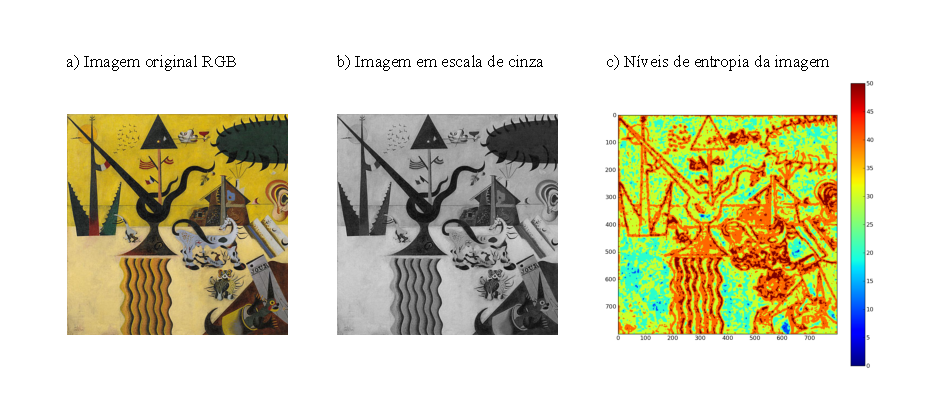
\includegraphics[scale=1]{figs/entrop}
        \fonteminha
\end{center}
\end{figure}

\subsection{Atributos espectrais}

Atributos espectrais envolvem o cálculo da densidade espectral para a
imagem total e para certos elementos da imagem, como colunas, linhas e
centroides. A densidade espectral da imagem total é dada pelo cálculo
da transformada de Fourier. Vale aqui introduzir tal conceito para se
chegar à definição de densidade espectral. Seja $f(x)$ uma função
contínua de uma variável real $x$, a transformada de Fourier
$\mathcal{F}\{f(x)\}$ é definida pela equação

\begin{equation}
  \mathcal{F}\{f(x)\} = F(u) = \int_{-\infty}^{+\infty} f(x) \exp[-2i\pi u x] dx
\end{equation}

\noindent com $i = \sqrt{-1}$. A partir de $F(u)$ pode-se obter a função
original $f(x)$ através da \emph{transformada inversa de Fourier}:

\begin{equation}
  \mathcal{F}^{-1}\{F(u)\} = f(x) = \int_{-\infty}^{+\infty} F(u) \exp[2i\pi u x] du.
\end{equation}

A transformada de Fourier de uma função real é geralmente complexa, e pode ser
expressa por

\begin{equation}
  F(u) = \Re(u) + \Im(u)i
  \label{eq:fourier_complexa}
\end{equation}

\noindent onde $\Re(u)$ e $\Im(u)$ são os componentes real e imaginário de
$F(u)$, respectivamente. É conveniente expressar a
equação~\ref{eq:fourier_complexa} em sua forma exponencial:

\begin{equation}
  F(u) = |F(u)|e^{\phi(u)i}
\end{equation}

\noindent onde $|F(u)| = \left[\Re^2(u) + \Im^2(u)\right]^{\frac{1}{2}}$ é o
\emph{espectro de Fourier} e
$\phi(u) = \tan^{-1}\left[\frac{\Im(u)}{\Re(u)}\right]$ o \emph{ângulo de
  fase}. Tomando-se o quadrado do espectro tem-se a \emph{densidade espectral},
também chamada de \emph{espectro de potência} de $f(x)$:

\begin{equation}
  P(u) = |F(u)|^2 = \Re^2(u) + \Im^2(u).
  \label{eq:densidade}
\end{equation}

A densidade espectral da imagem $I$ pode ser calculada com base na equação~\ref{eq:densidade}:

\begin{eqnarray}
  E = |\Re(X(I))|^2 + |\Im(X(I))|^2
\end{eqnarray}

\noindent onde $X$ é a transformada de Fourier de $I$ e a soma dos quadrados dos
módulos da parte real e imaginária de $X$ corresponde à energia espectral
procurada. Com base nessa medida, pode-se derivar as medidas de média e desvio
padrão das energias nas linhas, colunas, centroides e da imagem total:

\begin{eqnarray}
  \mathcal{A}_1 &=& \frac{\sum_j E_{(x,y)}}{N_y} \, \, \, \text{média das energias
    nas linhas $x$} \\
  \mathcal{A}_2 &=& \sqrt{\frac{\sum_y (E_{(x,y)} - \mu)^2}{N_y}} \, \, \,
  \text{desvio padrão das energias nas linhas $x$} \\
  \mathcal{A}_3 &=& \frac{\sum_x E_{(x,y)}}{N_x} \, \, \, \text{média das energias
    nas colunas $y$} \\
  \mathcal{A}_4 &=& \sqrt{\frac{\sum_x (E_{(x,y)} - \mu)^2}{N_x}} \, \, \,
  \text{desvio padrão das energias nas colunas $y$} \\
  \mathcal{A}_5 &=& \frac{\sum_y y E_{(x,y)}}{N_y} \, \, \, \text{centroide das energias
    nas linhas $x$} \\
  \mathcal{A}_6 &=& \frac{\sum_x i E_{(x,y)}}{N_x} \, \, \, \text{centroide das energias
    nas colunas $y$} \\
  \mathcal{A}_7 &=& \frac{\sum E_{(x,y)}}{N_x + N_y} \, \, \, \text{média das energias
    nas linhas $x$ e colunas $y$} \\
  \mathcal{A}_8 &=& \sqrt{\frac{\sum (E_{(x,y)} - \mu)^2}{N_x + N_y}} \, \, \,
  \text{desvio padrão das energias nas linhas $x$ e colunas $y$}
\end{eqnarray}

Essas mesmas medidas, que foram aplicadas à representação da imagem
original em níveis de cinza ($\mathcal{A}_{1-8}$), podem ser aplicadas
para cada uma das três imagens monocromáticas correspondentes a cada
canal RGB da imagem $I$, obtendo assim o conjunto $\mathcal{A}_{9-16}$
de atributos para o canal vermelho, conjunto de atributos
$\mathcal{A}_{17-24}$ para canal verde e $\mathcal{A}_{25-32}$ para o
canal azul.

\subsection{Atributos de textura}

Com o objetivo de analisar a textura das imagens, as 14 medidas
propostas por Haralick~\cite{haralick} são de interesse. Elas são
medidas ditas \emph{estatísticas de segunda ordem} pois são calculadas
a partir da matriz de coocorrência de níveis de cinza de uma dada
imagem $I$. Uma das vantagens dessa abordagem é levar em conta a
posição relativa de cada \textit{pixel} da imagem. Cada uma das 14 medidas
propostas procura caracterizar um aspecto de textura como contraste,
homogeneidade e complexidade.

Dada uma imagem $I$ com $N_G$ níveis de cinza, sua matriz de
coocorrência será uma matriz quadrada de dimensões $N_G \times N_G$
onde cada elemento $P_{\vec{d}}(i,j)$ representa a quantidade
de \textit{pixels} da imagem $I$ que possuem os níveis de cinza $i$ e
$j$, separados por uma distância numa certa direção e sentido,
determinado por $\vec{d}$. Para uma imagem, considera-se apenas o
posicionamento relativo entre cada \textit{pixel} e seus vizinhos
(i.e.\ \textit{pixels} adjacentes) e portanto, $\vec{d}$ poderá
assumir apenas 8 direções possíveis considerando os possíveis ângulos
$\beta \in \{0^o, 45^o, 90^o, 135^o, 180^o, 225^o, 270^o, 315^o\}$ que
tal vetor pode assumir dado que encontra-se ``aprisionado'' em uma
malha (i.e.\ possui vizinhança-8). Como trata-se de uma matriz de
coocorrência, esta é simétrica, e portanto o conjunto de possíveis
$\beta$ torna-se ainda menor. Por fim, dados os possíveis ângulos
$\beta \in \{0^o, 45^o, 90^o, 135^o\}$ e considerando os valores
$\{-1, 0, 1\}$ como domínio das coordenadas $x,y$ de $\vec{d}$, tem-se
o cálculo dos 14 atributos de Haralick para cada uma das seguintes
direções:

\begin{eqnarray}
  \beta = 0^o & \to & \vec{d} = (1, 0) \\
  \beta = 45^o & \to & \vec{d} = (1, 1) \\
  \beta = 90^o & \to & \vec{d} = (0, 1) \\
  \beta = 135^o & \to & \vec{d} = (-1, 1)
\end{eqnarray}

\noindent a tabela~\ref{tab:haralick} lista os 14 atributos de Haralick,
lembrando que estes são calculados para cada uma das 4 direções possíveis de
$\vec{d}$. Assim, essas medidas definem os $14 \cdot 4 = 56$ atributos seguintes
considerados nesse estudo, o conjunto $\mathcal{A}_{33-88}$.

\begin{table}
  \begin{center}
  \caption{\label{tab:haralick}Os 14 atributos de textura de Haralick,
    considerando: \\ $p(i,j) = P_{\vec{d}}(i,j)$, \\ $p_x(i) = \sum_{j=1}^{N_g}
    p(i,j)$, \\ $p_y(j) = \sum_{i=1}^{N_g} p(i,j)$, \\ $p_{x+y}(k=i+j) =
    \sum_{i=1}^{N_g}\sum_{j=1}^{N_g} p(i,j)$,  \\ $p_{x-y}(k=|i-j|) =
    \sum_{i=1}^{N_g}\sum_{j=1}^{N_g} p(i,j)$. \\ Ainda, $H(X)$ é a entropia de $X$
    e $\text{autoval}_2(X)$ é o segundo maior autovalor de $X$.}

  \begin{tabular}{l|l}
    \hline \hline
    Uniformidade      & $f_1 = \sum_{i=1}^{N_g}\sum_{j=1}^{N_g}
    p(i,j)^2$ \\ \\
    Contraste         & $f_2 = \sum_{i=1}^{N_g}\sum_{j=1}^{N_g} (i-j)^2 p(i,j)$
    \\ \\
    Correlação        & $f_3 = \frac{\sum_{i=1}^{N_g}\sum_{j=1}^{N_g} i j p(i,j)
      - \mu_x - \mu_y}{\sigma_x \sigma_y}$ \\ \\
    Variância         & $f_4 = \sum_{i=1}^{N_g}\sum_{j=1}^{N_g} (i-\mu)^2 p(i,j)$
    \\ \\
    Momento inverso da diferença & $f_5 = \sum_{i=1}^{N_g}\sum_{j=1}^{N_g}
    \frac{1}{1 + (i-j)^2} p(i,j)$ \\ \\
    Média da soma     & $f_6 = \sum_{k=2}^{2 N_g} k p_{x+y}(k)$ \\ \\
    Variância da soma     & $f_7 = \sum_{k=2}^{2 N_g} (k-f_6)^2 p_{x+y}(k)$ \\ \\
    Entropia da soma     & $f_8 = -\sum_{k=2}^{2 N_g} p_{x+y}(k)
    log\left(p_{x+y}(k)\right)$ \\ \\
    Entropia             & $f_9 = -\sum_{i=1}^{N_g}\sum_{j=1}^{N_g} p(i,j)
    log\left(p(i,j)\right)$ \\ \\
    Variância da diferença & $f_{10} = \text{var}(p_{x-y})$ \\ \\
    Entropia da diferença     & $f_{11} = -\sum_{k=0}^{N_g - 1} p_{x-y}(k)
    log\left(p_{x-y}(k)\right)$ \\ \\
    Medida de correlação (1)  & $f_{12} = \frac{f_9 +
      \sum_{i=1}^{N_g}\sum_{j=1}^{N_g} p(i,j) log\left[p_x(i)
        p_y(j)\right]}{max\{H(p_x(i)), H(p_y(j))\}}$ \\ \\
    Medida de correlação (2)  & $f_{13} = \sqrt{1-exp\left[ -2
        \left(\left(-\sum_{i=1}^{N_g}\sum_{j=1}^{N_g} p_x(i) p_y(j) log\left(p_x(i)
            p_y(j)\right)\right) - f_9\right)\right]}$ \\ \\
    Coeficiente de correlação máxima & $f_{14} =
    \sqrt{\text{autoval}_2\left(-\sum_{k=1}^{N_g} \frac{p(i,k) p(j,k)}{p_x(i) p_y(j)} \right)}$ \\ \hline \hline
\end{tabular}
\fonteminha
\end{center}
\end{table}

\subsection{Atributos de contorno e forma}

Após a identificação dos componentes conexos e seu pós-processamento,
pode-se partir para a descrição da forma de tais componentes. A
curvatura é um destes descritores. Trata-se de um atributo que mensura
a mudança de direção ``relativa'' entre dois pontos
conectados.~\cite{luciano} Esse descritor tem uma motivação biológica
interessante relacionada com o sistema de visão humano --- i.e.\ o
reconhecimento de objetos é relacionado à identificação de cantos e
pontos de alta curvatura. Esses pontos possuem mais informação sobre a
forma do objeto do que linhas retas ou curvas suaves. Dessa forma, a
curvatura é um atributo interessante para uso na caracterização das
pinturas consideradas nesse estudo, pois pinturas como as de Miró
parecem possuir maior quantidade de linhas retas (com poucas curvas)
do que as pinturas barrocas, por exemplo. A curvatura de uma forma é
calculada usando os seguintes descritores de Fourier e esquematizada
na figura~\ref{fig:curvatura}.

\begin{figure}[h!]
\begin{center}
      \caption{\textit{a)} Imagem da pintura original. \textit{b)} Uma região
        segmentada da pintura. \textit{c)} A curvatura extraída a partir
        da região segmentada. \textit{d)} A curva paramétrica $k(t)$ dado um
        limiar em particular, com os picos em destaque.}
        \label{fig:curvatura}
        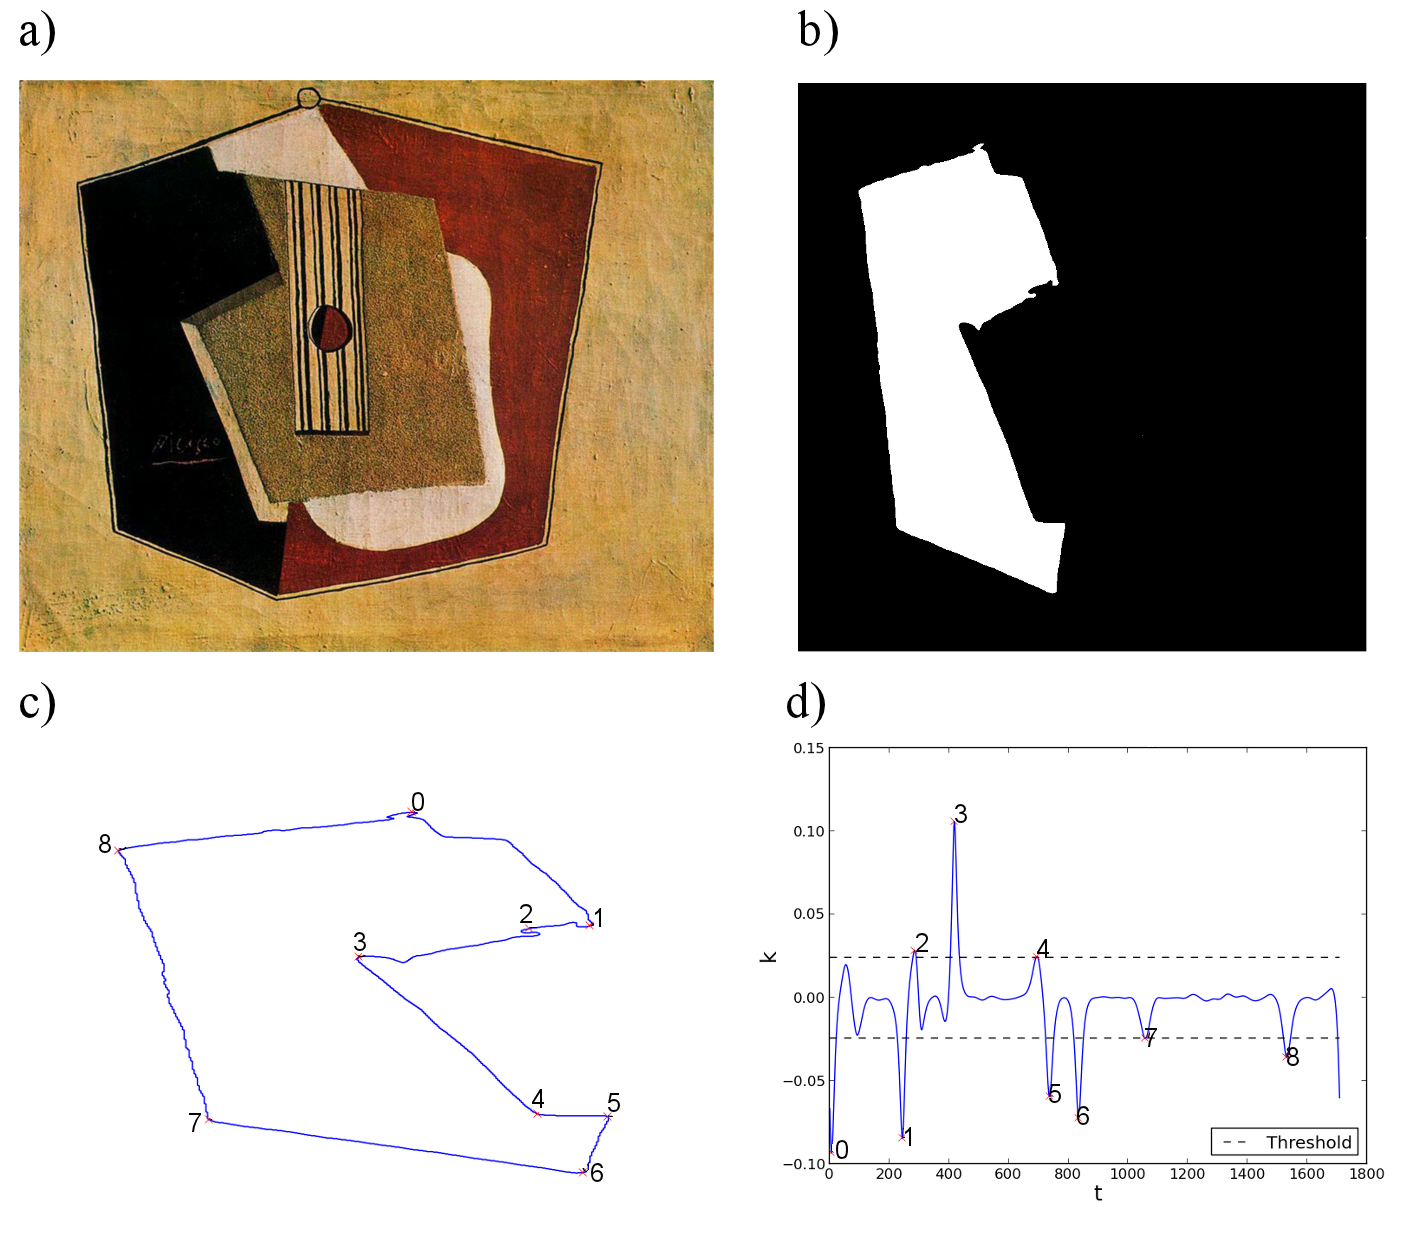
\includegraphics[width=\columnwidth]{figs/curvatura}
       \fonteminha
\end{center}
\end{figure}

A curvatura $k(t)$ de uma curva paramétrica $c(t) = (x(t), y(t))$ é definida como:

\begin{equation}
k(t) = \frac{\dot{x}(t)\ddot{y}(t)-\dot{y}(t)\ddot{x}(t)} {(\dot{x}(t)^2+\dot{y}(t)^2)^\frac{3}{2}}
\label{eq:curvatura}
\end{equation}

\noindent onde $\dot{x}(t)$, $\dot{y}(t)$, $\ddot{x}(t)$ e
$\ddot{y}(t)$ são respectivamente as derivadas de primeira e segunda
ordem dos parâmetros $x(t)$ e $y(t)$ da curva $k(t)$. Essas derivadas
podem ter seus valores estimados através da transformada de Fourier e
do teorema da convolução:~\cite{papoulis}

\begin{equation}
\dot{x} = \Im^{-1}(2\pi i \omega X(\omega))
\end{equation}
\begin{equation}
\dot{y} = \Im^{-1}(2\pi i \omega Y(\omega))
\end{equation}
\begin{equation}
\ddot{x} = \Im^{-1}(-(2\pi\omega)^2 X(\omega))
\end{equation}
\begin{equation}
\ddot{y} = \Im^{-1}(-(2\pi\omega)^2 Y(\omega))
\end{equation}

\noindent onde $\Im^{-1}$ é a transformada inversa de Fourier, $X$ e $Y$ a
transformada de Fourier de $x$ e $y$ respectivamente, $\omega$ é a frequência angular
e $i$ a unidade imaginária.

O cálculo das derivadas $(\dot{x}(t), \dot{y}(t))$ e $(\ddot{x}(t),
\ddot{y}(t))$ do sinal $t$ através do cálculo da transformada de
Fourier --- i.e.\ por um método numérico de diferenciação --- acaba
por realçar ruídos de alta frequência. Pode-se compensar este efeito
através de uma filtragem,~\cite{luciano,luciano2010} onde as funções
diferenciadas durante o processo são suavizadas a partir da convolução
de um filtro gaussiano aplicado ao sinal à ser diferenciado. Ou seja,
a diferenciação por Fourier acaba por criar um filtro passa-altas,
necessitando de um filtro passa-baixas para amenizar o ruído. Tal
filtro gaussiano é definido por

\begin{equation}
g(t) = \frac{1}{2\pi\sigma^2} exp \left( -\frac{t^2}{2\sigma^2}\right)
\end{equation}

\noindent e sua transformada de Fourier é dada por

\begin{equation}
G(\omega) = exp \left( \frac{-(2\pi)^2\omega^2}{(2/\sigma)^2} \right)
\end{equation}

Utilizando-se o teorema da convolução é possível aplicar o filtro
gaussiano $g(t)$ ao sinal a ser diferenciado:

\begin{equation}
\hat{\dot{x}}(t) = \dot{x} \ast g(t) = \Im^{-1}\left( \dot{X}(\omega) G(\omega) \right)
\end{equation}

\begin{equation}
\hat{\dot{y}}(t) = \dot{y} \ast g(t) = \Im^{-1}\left( \dot{Y}(\omega) G(\omega) \right)
\end{equation}

\begin{equation}
\hat{\ddot{x}}(t) = \ddot{x} \ast g(t) = \Im^{-1}\left( \ddot{X}(\omega) G(\omega) \right)
\end{equation}

\begin{equation}
\hat{\ddot{y}}(t) = \ddot{y} \ast g(t) = \Im^{-1}\left( \ddot{Y}(\omega) G(\omega) \right)
\end{equation}

\noindent obtendo assim a diferenciação multi-escala de primeira e
segunda ordem $(\hat{\dot{x}}(t),\hat{\dot{y}}(t))$ e
$(\hat{\ddot{x}}(t),\hat{\ddot{y}}(t))$ para $x(t)$ e $y(t)$, agora
sim usadas para o cálculo de $k(t)$ (eq.~\ref{eq:curvatura}) sem a
presença de possíveis ruídos de alta-frequência.

É importante notar que um \emph{pico} é definido como um ponto de alta
curvatura. Um ponto $a$ é considerado um pico se sua curvatura $k(a)$
satisfazer os seguintes critérios:

\begin{eqnarray}
	k(a) & > & k(a-1) \\
	k(a) & > & k(a+1)
\end{eqnarray}

Ou seja, um ponto $a$ é dito pico se sua curvatura $k(a)$ for maior
que seus vizinhos anteriores e posteriores. Isto é suficiente para
determinar todos os picos contidos no contorno de uma forma
qualquer. Porém, é preciso controlar quais picos são interessantes e
quais devem ser descartados. Desta forma, deve-se incluir um novo
critério:

\begin{eqnarray}
  k(a) & > & \tau
\end{eqnarray}

\noindent ou seja, apenas pontos com curvaturas maiores que o limiar
$\tau$ serão consideradas. Este limiar, por sua vez, pode ser definido
como

\begin{equation}
	\text{mediana}\left(k\right) \cdot \gamma 
\end{equation}

\noindent onde $\gamma$ equivale a um fator obtido empiricamente com valores que
revelam um determinado nível de detalhe de curvatura. Quanto maior o valor de
$\gamma$, mais picos de curvatura e vice-versa.

Tendo-se definido a curvatura $k(t)$ e um pico de curvatura $a$, pode-se partir
para a definição de uma série de atributos. A média e o desvio padrão das
distâncias geométricas entre um pico $a_{i}$ e seu próximo pico $a_{i+1}$
compõem os atributos $\mathcal{A}_{89}$ e $\mathcal{A}_{90}$, usados neste
estudo:

\begin{eqnarray}
  \mathcal{A}_{89} & = & \text{média}(\sqrt{(a_{i} - a_{i+1})^2}) \\
  \mathcal{A}_{90} & = & \text{desvio padrão}(\sqrt{(a_{i} - a_{i+1})^2})
\end{eqnarray}

\noindent Também pode-se considerar tal distância dada em coordenadas do \textit{pixel}
da imagem associada ao pico $a$, o que leva aos atributos $\mathcal{A}_{91}$ e
$\mathcal{A}_{92}$, que representam, respectivamente, a média e desvio padrão da
distância em \textit{pixels} entre um pico $a_{i}$ e seu próximo pico $a_{i+1}$.

A simples quantidade de picos $a$ de uma dada curvatura $k(t)$ revela um novo
atributo:

\begin{eqnarray}
  \mathcal{A}_{93} & = & \text{tam}(\{a_{i}, a_{i+1}, ..., a_{N}\})
\end{eqnarray}

\noindent sendo \textit{tam} o tamanho do conjunto de todos os picos $a$ de uma
curvatura calculada. Da mesma forma, a quantidade de elementos $k(t)$ da
curvatura permite saber o perímetro em \textit{pixels} da região conexa:

\begin{eqnarray}
  \mathcal{A}_{94} & = & \text{tam}(\{k(t_{i}), k(t_{i+1}), ..., k(t_{N})\})
\end{eqnarray}

Ainda, somando-se todos os elementos da região conexa $C_i = i$, onde $i$
representa o rótulo da região, tem-se a área desta região, em \textit{pixels}, e portanto
define-se um novo atributo $\mathcal{A}_{95}$. A razão entre o perímetro e a
área, ambos em \textit{pixels}, oferece mais um atributo:

\begin{eqnarray}
  \mathcal{A}_{96} & = & \frac{(\mathcal{A}_{94})^2}{\mathcal{A}_{95}}
\end{eqnarray}

\noindent essa razão indica quanto uma forma se aproxima de um círculo.

A quantidade $C_N$ de regiões conexas $C_i$ também caracteriza um atributo de
interesse $\mathcal{A}_{97}$. Trata-se de um atributo importante pois indica o
quanto uma imagem é complexa em relação ao número de elementos que a compõe. Por exemplo, as pinturas de Pollock possuem um número muito maior de componentes do
que a maioria dos demais pintores.

A área da região convexa de uma forma fornece outro atributo. É calculado
através do algoritmo \textit{convex-hull}~\cite{luciano} e define o atributo
$\mathcal{A}_{98}$. A razão entre a área da região convexa e da região original
do componente ($\mathcal{A}_{95}$) indicam outra medida de circularidade, ou o
quanto o componente possui uma forma rica em curvas acentuadas:

\begin{eqnarray}
  \mathcal{A}_{99} & = & \frac{\mathcal{A}_{98}}{\mathcal{A}_{95}}
\end{eqnarray}

O conjunto de todos os 100 atributos $\mathcal{A}_i$ discutidos estão sumarizados na
tabela~\ref{tab:atributos}. É importante ressaltar que cada imagem de pintura
acaba apresentando um número arbitrário de regiões conexas após os processos de
segmentação e pós-processamento. Desta forma, para cada pintura tem-se um ou
mais valores para os atributos $\mathcal{A}_{89-99}$, e portanto a média destes
valores foi tomada para representar cada um destes atributos para uma dada imagem.

\begin{table}
  \begin{center}
  \caption{\label{tab:atributos}Sumário de todos os 100 atributos utilizados
    neste estudo, considerando detalhes de contraste, textura (descritas pelas
    medidas de entropias e energias, assim como as medidas de Haralick) e forma
    (descritas pelas medidas de curvatura e medidas geométricas como perímetro,
    área e sua razão).}

  \begin{tabular}{l|l}
    \hline \hline
    \textbf{$\mathcal{A}_i$} & \textbf{Descrição} \\
    \hline

    $\mathcal{A}_0$ & 
    Entropia da imagem em tons de cinza \\
    
    $\mathcal{A}_1$ & 
    Média das energias nas linhas $x$ da imagem em tons de cinza \\
    %$\mathcal{A}_1  = \frac{\sum_j E_{(i,j)}}{N_j}$ \\

    $\mathcal{A}_2$ &
    Desvio padrão das energias nas linhas $x$ da imagem em tons de cinza \\
    %$\mathcal{A}_2 = \sqrt{\frac{\sum_j (E_{(i,j)} - \mu)^2}{N_j}}$ \\

    $\mathcal{A}_3$ &
    Média das energias nas colunas $y$ da imagem em tons de cinza \\
    %$\mathcal{A}_3 = \frac{\sum_i E_{(i,j)}}{N_i}$ \\

    $\mathcal{A}_4$ &
    Desvio padrão das energias nas colunas $y$ da imagem em tons de cinza \\
    %$\mathcal{A}_4 = \sqrt{\frac{\sum_i (E_{(i,j)} - \mu)^2}{N_i}}$ \\

    $\mathcal{A}_5$ &
    Centroide das energias nas linhas $x$ da imagem em tons de cinza \\
    %$\mathcal{A}_5 = \frac{\sum_j j E_{(i,j)}}{N_j}$ \\

    $\mathcal{A}_6$ &
    Centroide das energias nas colunas $y$ da imagem em tons de cinza \\
    %$\mathcal{A}_6 = \frac{\sum_i i E_{(i,j)}}{N_i}$ \\

    $\mathcal{A}_7$ &
    Média das energias nas linhas $x$ e colunas $y$ da imagem em tons de cinza \\
    %$\mathcal{A}_7 = \frac{\sum E_{(i,j)}}{N_i + N_j}$ \\

    $\mathcal{A}_8$ &
    Desvio padrão das energias nas linhas $x$ e colunas $y$ da imagem em tons de
    cinza \\
    %$\mathcal{A}_8 = \sqrt{\frac{\sum (E_{(i,j)} - \mu)^2}{N_i + N_j}}$ \\

    $\mathcal{A}_{9-16}$ &
    As mesmas medidas $\mathcal{A}_{1-8}$ mas aplicadas à banda vermelha da
    imagem \\

    $\mathcal{A}_{17-24}$ &
    As mesmas medidas $\mathcal{A}_{1-8}$ mas aplicadas à banda verde da
    imagem \\

    $\mathcal{A}_{25-32}$ &
    As mesmas medidas $\mathcal{A}_{1-8}$ mas aplicadas à banda azul da
    imagem \\

    $\mathcal{A}_{33-46}$ &
    As 14 medidas de textura de Haralick para a direção $\beta = 0^o$ ou $\vec{d} = (1, 0)$ \\

$\mathcal{A}_{47-60}$ &
    As 14 medidas de textura de Haralick para a direção $\beta = 45^o$ ou $\vec{d} = (1, 1)$ \\

$\mathcal{A}_{61-74}$ &
    As 14 medidas de textura de Haralick para a direção $\beta = 90^o$ ou $\vec{d} = (0, 1)$ \\

$\mathcal{A}_{75-88}$ &
    As 14 medidas de textura de Haralick para a direção $\beta = 135^o$ ou $\vec{d} = (-1, 1)$ \\

    $\mathcal{A}_{89}$ &
    Média das distâncias (euclidiana) entre os picos de curvatura \\

    $\mathcal{A}_{90}$ &
    Desvio padrão das distâncias (euclidiana) entre os picos de curvatura \\

    $\mathcal{A}_{91}$ &
    Média das distâncias (em \textit{pixels} do contorno) entre os picos de curvatura \\

    $\mathcal{A}_{92}$ &
    Desvio padrão das distâncias (em \textit{pixels} do contorno) entre os picos de
    curvatura \\

    $\mathcal{A}_{93}$ &
    Quantidade de picos de curvatura \\

    $\mathcal{A}_{94}$ &
    Perímetro da curvatura \\

    $\mathcal{A}_{95}$ &
    Área da região conexa \\

    $\mathcal{A}_{96}$ &
    Razão entre o perímetro e a área da região \\

    $\mathcal{A}_{97}$ &
    Quantidade de segmentos de uma pintura \\

    $\mathcal{A}_{98}$ &
    Área da região convexa \\

    $\mathcal{A}_{99}$ &
    Razão entre a área da região convexa e a área da região conexa original \\

    \hline \hline
    \end{tabular}
    \fonteminha
  \end{center}
\end{table}

\clearpage
\section{Análise de atributos e redução de dimensionalidade}
\label{sec:fund:reducao}

Na maioria das rotinas de análises de dados, a quantidade de atributos leva à
necessidade de selecionar quais atributos são mais relevantes ao objetivo
previsto (e.g.\ garantir máximo agrupamento das amostras em certas classes) e
reduzir a dimensionalidade das amostras a um ponto que se consiga
visualizá-las. Essas necessidades estão presentes também neste estudo e alguns
métodos foram selecionados para supri-las.

Existe um grande número de métodos para a identificação dos melhores
atributos, aqui dois deles são descritos: matriz de espalhamento e LDA
(\textit{Linear Discriminant Analysis}).~\cite{fisher,luciano,jain}
Esse último também pode ser utilizado para a redução da dimensão da
matriz de entrada, e é portanto descrito juntamente com outro método
para redução de dimensionalidade, o PCA (\textit{Principal Components
Analysis}).~\cite{luciano,dunteman}

O método conhecido como matrizes de espalhamento procura encontrar a melhor
razão de Fisher, que é um indicador quantitativo de quanto duas ou mais classes
estão apresentando menor covariância interna (agrupamento) e maior covariância
entre as classes (dispersão). Ou seja, busca-se a projeção que mais separa as
classes umas das outras.~\cite{fisher,luciano}

Para todas as $N$ amostras (no caso, pinturas), considerando todas as possíveis
combinações de pares de atributos $F_{N, a}$ e $F_{N, b}$, as matrizes de
espalhamento $S_{inter}$ e $S_{intra}$ são calculadas com $K$ classes (no caso,
$K = 12$ para 12 pintores), uma classe $C_i$ para cada pintor:

\begin{equation}
S_{intra} = \sum_{i=1}^K S_i
\end{equation}

\begin{equation}
S_{inter} = \sum_{i=1}^K N_i(\vec{\mu_i} - \vec{M})(\vec{\mu_i} - \vec{M})^T
\end{equation}

\noindent sendo $N_i$ o número de amostras para a classe $C_i$ e a matriz de
espalhamento para a classe $C_i$ definida como

\begin{equation}
S_i = \sum_{i \in C_i} (\vec{f_i} - \vec{\mu_i})(\vec{f_i} - \vec{\mu_i})^T
\end{equation}

\noindent onde $\vec{f_i}$ é uma amostra da matriz de atributos $F$ cujas linhas
e colunas correspondem às amostras e seus atributos $F = \left[ \leftarrow
  f_i^T \rightarrow \right]$ e $\vec{\mu_i}$ e $\vec{M}$ são os vetores de média
dos atributos para as amostras da classe $C_i$ e para todas as amostras,
respectivamente:

\begin{equation} 
\vec{\mu_i} = \frac{1}{N_i} \sum_{i \in C_i} \vec{f_i}
\end{equation}

\begin{equation}
\vec{M} = \frac{1}{N} \sum_{i=1}^N \vec{f_i}
\end{equation}

O traço da razão entre as matrizes intra- e interclasse resulta na razão de
Fisher, a constante:

\begin{equation} \label{eq:alpha}
\alpha = \mathrm{tr}(S_{inter} S_{intra}^{-1})
\end{equation}

Se ao invés de calcular o traço for calculado os autovalores e autovetores da
razão das matrizes, tem-se a projeção que melhor separa as classes, ou seja, o LDA:

\begin{equation} \label{eq:lda}
\text{eig}(S_{inter} S_{intra}^{-1})
\end{equation}

\noindent onde $\mathrm{eig}$ corresponde ao cálculo dos autovetores e
autovalores do produto entre as matrizes de espalhamento. Ao tomar os
autovetores dos maiores autovalores, em módulo, tem-se tal projeção. É por isso
que o LDA pode ser concebido como um método de redução de dimensão, reduzindo os
$N$ atributos a um número de atributos $r < N$ (geralmente $r \le 3$ para
possibilitar a projeção em 2 ou 3 dimensões visíveis) que melhor separam as
classes.

Convém aqui abordar um outro método de redução de dimensionalidade, o PCA, que
lembra o LDA. No PCA, se está interessado em calcular os autovalores e
autovetores que mais correlacionam os dados em questão. Para isso, toma-se a
matriz de atributos $F$ e calcula-se sua matriz de covariância, que nada mais é
que a operação de covariância aplicada a cada dimensão $i$ de uma matriz $X$
qualquer. Considerando os momentos estatísticos básicos, a matriz de covariância
$C^{n \times n}(X)$ dadas $n$ dimensões de $X$ é dada por

\begin{equation}
  C^{n \times n}(X) = \left(
    \begin{array}{cccc}
      cov(x_1,x_1) & cov(x_1,x_2) & \dots  & cov(x_1,x_n) \\
      cov(x_2,x_1) & cov(x_2,x_2) & \dots  & cov(x_2,x_n) \\
      \vdots       & \vdots       & \vdots & \vdots       \\
      cov(x_n,x_1) & cov(x_n,x_2) & \dots  & cov(x_n,x_n)
    \end{array}
  \right)
\end{equation}

\noindent onde $x_i$ é a $i$-ésima dimensão da matriz $X$.

Novamente, calculando os autovalores (e seus respectivos autovetores) da matriz
de covariância $C^{n \times n}(F)$ e tomando os autovetores dos maiores
autovalores, em módulo, tem-se os \emph{componentes principais}

\begin{equation}
 V = \bigg(autovetor_0 \; autovetor_1 \; \dots \; autovetor_n \bigg)
\end{equation}

\noindent que formarão uma base para a projeção dos dados com maior correlação
possível através da multiplicação da matriz original $F$ com os componentes
principais $V$, ambos transpostos:

\begin{equation}
 D \; = V^T \times F^T
\end{equation}

\noindent ou seja, $D$ é a base que mais ``reúne características'' dos demais
atributos. Tomando-se apenas estes $r < N$ atributos, tem-se portanto uma
redução na dimensão. Os autovalores indicam o quanto cada
atributo contribui para a correlação.~\cite{luciano}

\subsection{Validação cruzada}

A projeção obtida pelo método LDA através da equação~\ref{eq:lda} não
garante a classificação dos dados, visto que as classes são conhecidas
previamente (fazendo com que o método LDA seja utilizado como parte de
um método supervisionado de classificação). Assim, é preciso validar
tal projeção obtida frente a outras possíveis escolhas dos conjuntos
de treinamento e teste.

Um procedimento comum neste caso é a validação cruzada ou
\textit{cross validation}. Nesta pesquisa utilizou-se o método de validação cruzada conhecido como \textit{repeated random sub-sampling validation}. Trata-se de um método bastante simples,
onde os dados de amostra são divididos em dois grupos: um
\emph{conjunto de treinamento} e um \emph{conjunto de teste}. Os elementos de ambos os grupos são selecionados aleatoriamente. O método
LDA é então aplicado ao conjunto de treinamento, obtendo-se a projeção
(eq.~\ref{eq:lda}). O LDA é aplicado em seguida ao conjunto de teste,
mas utilizando a projeção obtida para o conjunto de treinamento (i.e.\
os mesmos autovetores). Conta-se agora quais amostras do conjunto de
teste foram projetadas próximas ao conjunto de treinamento, e quais
estão distantes. Essa contagem revela se o conjunto de treinamento
condiz com o esperado e desta forma, valida o método LDA aplicado.~\cite{luciano}

Uma forma interessante de visualizar a validação cruzada é através da
\emph{matriz de confusão}, representada na
figura~\ref{fig:confusa}. Cada linha da matriz de confusão representa
uma classe $C_i$ do grupo de treinamento (no caso deste estudo, as
classes correspondem a cada um dos pintores analisados) e cada coluna
representa uma classe $\hat{C_i}$ do grupo de teste. Cada elemento da
matriz representa a contagem de amostras pertencentes a uma
determinada classe, ou seja, as amostras de $C_i$ que deveriam ser
classificadas como $\hat{C_i}$. Desta forma, espera-se que a diagonal
principal desta matriz esteja o mais próximo possível do número máximo
de elementos para cada classe. Ou seja, elementos de uma classe $C_1$
devem ser classificados como pertencentes a esta classe, e não a
qualquer outra classe. Um exemplo de matriz de confusão para o método
LDA pode ser visto na figura~\ref{fig:cm} da seção~\ref{subsec:lda} de
resultados deste estudo.

\begin{figure}[ht!]
\begin{center}
\caption{\label{fig:confusa} Esquema representando uma matriz de
  confusão. Deseja-se que a diagonal principal possua valores próximos
  ao número máximo de elementos em cada classe $C_i$, caracterizando
  assim uma boa classificação. $C_i$ é uma classe do conjunto de
  treino e $\hat{C_i}$ uma classe do conjunto de teste.}

\vspace{15pt}

\begin{tikzpicture}[thick]
\draw [fill=red,opacity=0.3] (0,0) grid (4,4) rectangle (0,0);
% classes
\node at (-0.5,3.5) {$C_1$};
\node at (-0.5,2.5) {$C_2$};
\node[rotate=90] at (-0.5,1.5) {...};
\node at (-0.5,0.5) {$C_K$};

\node at (0.5,4.5) {$\hat{C_1}$};
\node at (1.5,4.5) {$\hat{C_2}$};
\node at (2.5,4.5) {...};
\node at (3.5,4.5) {$\hat{C_K}$};

% diagonal principal
\node [fill=green, minimum size=1.0cm] at (0.5,3.5) {};
\node [fill=green, minimum size=1.0cm] at (1.5,2.5) {};
\node [fill=green, minimum size=1.0cm] at (2.5,1.5) {};
\node [fill=green, minimum size=1.0cm] at (3.5,0.5) {};

% labels
\node at (2,5.5) {Conjunto de teste};
\node [rotate=90] at (-1.5,2) {Conjunto de treinamento};

\end{tikzpicture}
\vspace{15pt}
\fonteminha
\end{center}
\end{figure}

Conhecendo-se a quantidade de amostras que foram classificadas corretamente e aquelas que não o foram, é possível calcular a acurácia da classificação, definida como

\begin{equation}
  acc(C_i, \hat{C_i}) = \frac{1}{N_s} \sum_{j=0}^{N_s-1} \textbf{1}(\hat{c_j} = c_j)
\end{equation}

\noindent onde $N_s$ é o número de amostras para uma classe $C_i$,
$c_j$ é uma amostra pertencente à $C_i$ e $\hat{c_j}$ é uma amostra
pertencente à $\hat{C_i}$. Ainda, a função $\textbf{1}$ é a função
característica ou indicadora, que indica se um elemento pertence ao
conjunto $Q$ (assumindo o valor 1) ou não (assumindo o valor 0), ou
seja:

\begin{equation}
  \textbf{1}(x) = \left\{
     \begin{array}{lr}
       1 & : x \in Q \\
       0 & : x \notin Q
     \end{array}
   \right.
\end{equation}

Assim, a acurácia pode ser interpretada como a fração das amostras que
foram classificadas como corretas para um determinado grupo de treino
e teste.

%%%%%%%%%%%%%%%%%%%%%%%%%%%%%%%%%%%%%%%%%%%%%%%%%%%%%%%%%%%%%%%%%%%%%%%%%%%
%%%%%%%%%%%%%%%%%%%%%%%%%%%%%%%%%%%%%%%%%%%%%%%%%%%%%%%%%%%%%%%%%%%%%%%%%%%

%\afterpage{\blankpage}
\chapter{Desenvolvimentos e resultados}
\label{chap:resultados}

% aqui começa o conteúdo do artigo

\section{Pintores escolhidos}

Para a análise foram selecionados 12 pintores de relevância
histórica. Esse grupo abrange os estilos artísticos que vão do período
Barroco aos movimentos da Arte Moderna. Seis dos pintores representam
o período Barroco enquanto os 6 restantes representam movimentos modernos. O grupo é apresentado na tabela~\ref{tab:painters}
juntamente com seu estilo e período ou movimento artístico mais
representativo. É de conhecimento que pintores como Picasso
demonstraram mais de um estilo durante a vida. Porém, para tal
análise, foi escolhido apenas o estilo pelo qual melhor se conhece e
define o artista. No caso de Picasso, apenas pinturas de sua fase
Cubista (de 1909 a 1912) foram escolhidas, com o objetivo de
representar este movimento. Destaca-se que a escolha de dois períodos
distantes --- cerca de 218 anos separam o período Barroco dos
movimentos da Arte Moderna --- é proposital. A história da Arte assim
como a análise estética das pinturas de ambos períodos revela
características contrastantes, porém tais afirmações são
qualitativas. Neste estudo, fez-se tal escolha justamente com o
objetivo de refutar ou afirmar estas observações, mas agora com base
em medidas quantitativas.

\begin{table}[h!]
\begin{center}
\caption{\label{tab:painters} Pintores escolhidos para a análise, exibidos em
  ordem cro\-no\-ló\-gi\-ca, juntamente com o estilo artístico que melhor
  representa. Divididos em dois grupos: 6 pintores barrocos e 6 pintores modernos.}

\begin{tabular}{l|l|l}
\hline \hline

 \textbf{Artistas}                      & \textbf{Estilos/movimentos/períodos mais marcantes} & \textbf{Período cronológico} \\ 
 
 \hline

 Caravaggio                    & Barroco & 1593 - 1610 \\
 Frans Hals                    & Barroco, Idade de ouro Holandesa & 1620 - 1660\\
 Nicolas Poussin               & Barroco, Classicismo & 1620 - 1660\\
 Diego Velázquez           & Barroco & 1618 - 1660\\
 Rembrandt                     & Barroco, Idade de ouro Holandesa, Realismo & 1632 - 1650\\
 Johannes Vermeer              & Barroco, Idade de ouro Holandesa & 1632 - 1670\\
 
 \hline
 
 Vincent van Gogh              & Pós-Impressionismo & 1888 - 1890\\
 Wassily Kandinsky             & Expressionismo, Arte abstrata & 1922 - 1944\\
 Henri Matisse                 & Modernismo, Fauvismo & 1904 - 1910\\
 Pablo Picasso                 & Cubismo & 1909 - 1912\\
 Joan Miró                 & Surrealismo, Dada & 1922 - 1958\\
 Jackson Pollock               & Expressionismo abstrato & 1947 - 1950\\

\hline \hline
\end{tabular}
\fonteminha
\end{center}
\end{table}


\section{Corpus de pinturas}

Para cada pintor, foram consideradas 20 imagens de suas pinturas,
obtidas de arquivos em domínio público, organizados pela
\textit{Wikipedia}. Uma amostra dessas pinturas e seu respectivo ano de criação
está listada na tabela~\ref{tab:paintings}. Todas as 240 pinturas são
apresentadas em forma de galeria no apêndice~\ref{cap:ap-galeria}. Os
arquivos de imagem das pinturas assim como o código-fonte que
implementa esta análise encontram-se disponíveis online em
\url{http://github.com/automata/ana-pintores} e no
apêndice~\ref{cap:ap-tutorial} há instruções de sua instalação e uso.

\begin{table}[h!] 
  \begin{center}
  \caption{\label{tab:paintings} Algumas das 240 pinturas juntamente
    com a data de sua criação. Todas as pinturas usadas no estudo
    estão apresentadas em forma de galeria no
    apêndice~\ref{cap:ap-galeria}.}

\begin{tabular}{l|l|l}
\hline \hline

 \textbf{Pintores} & \textbf{Título da obra}                       & \textbf{Ano de criação} \\ 
 
 \hline

 Caravaggio          & Músicos & 1595 \\
                     & Judite decapitando Holofernes & 1598 \\
                     & Davi com a cabeça de Golias & 1610 \\
                      
 Frans Hals          & Retrato de uma mulher desconhecida & 1618/20 \\
                     & Retrato de Paulus van Beresteyn & 1620s \\
                     & Retrato de Stephanus Geeraerdts & 1648/50 \\

 Nicolas Poussin     & Vênus e Adônis & 1624 \\
                     & Céfalo e Aurora & 1627 \\
                     & Ácis e Galateia & 1629 \\
 
 Diego Velázquez     & Três músicos & 1617/18 \\
                     & O almoço & 1618 \\
                     & La mulatto & 1620 \\
 
 Rembrandt           & O vendedor de óculos (visão) & 1624/25 \\
                     & Os três cantores (audição) & 1624/25 \\
                     & Balaão e o burro & 1626 \\

Johannes Vermeer    & A leiteira & 1658 \\
                    & O astrônomo & 1668 \\
                    & Garota com brincos de pérola & 1665 \\
                    
\hline                
                    
Vincent van Gogh    & Noite estrelada sobre o Ródano & 1888 \\
                    & A noite estrelada & 1889 \\
                    & Auto-retrato com chapéu de palha & 1887/88 \\

Wassily Kandinsky   & Em branco II & 1923 \\
                    & Composição X & 1939 \\
                    & Pontos & 1920 \\

Henri Matisse       & Auto-retrato em uma camiseta listrada & 1906 \\
                    & Retrato de Madame Matisse & 1905 \\
                    & A dança (primeira versão) & 1909 \\

Pablo Picasso       & Les Demoiselles d'Avignon & 1907 \\
                    & Guernica & 1937 \\
                    & Dora Maar au Chat & 1941 \\

Joan Miró       & O fazendeiro & 1921/22 \\
                    & O campo lavrado & 1923/24 \\
                    & Bleu II & 1961 \\

Jackson Pollock     & No. 5 & 1948 \\
                    & Ritmo de outono & 1950 \\
                    & Pólos azuis & 1952 \\

\hline \hline
\end{tabular}
\fonteminha
\end{center}
\end{table}


\section{Análise de imagens para extração de atributos}
\label{sec:analiseimagens}

Todas as 240 imagens foram cortadas em janelas de $800\times800$
\textit{pixels}. Esta janela quadrada foi posicionada com seu ponto superior
mais à esquerda equivalendo ao ponto superior mais à esquerda da
pintura (figura~\ref{fig:janelamento}). As imagens que possuíam
dimensões menores que $800\times800$ foram escaladas para tal
dimensão, mantendo o mesmo aspecto da imagem original em todas as
pinturas.

\begin{figure}[h!]
\begin{center}
        \caption{Pré-processamento para recorte das imagens originais em
        janelas de dimensão $800\times800$. \textit{a)} a imagem
        original, \textit{b)} a janela em destaque, \textit{c)} a
        imagem de dimensões $800\times800$ utilizada neste
        estudo. Embora se percam detalhes da imagem original, o
        janelamento é necessário para facilitar o processamento ao se
        utilizar uma dimensão única para as imagens.}
        \label{fig:janelamento}
        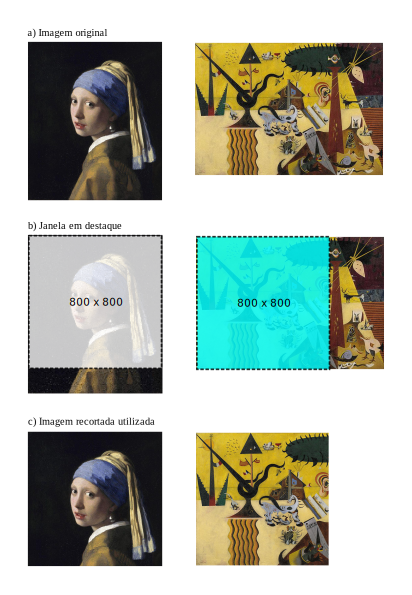
\includegraphics[scale=0.9]{figs/passos_janelamento}
      \fonteminha
\end{center}
\end{figure}

Em seguida, as imagens foram pré-processadas aplicando-se equalização
de histograma e filtro por mediana com janela de vizinhança-8
(figura~\ref{fig:eq}), ambas descritas na subseção~\ref{sec:preproc}.

\begin{figure}[ht!]
\begin{center}
         \caption{Pré-processamento utilizando equalização de histograma
        e filtro por mediana com janela de vizinhança-8. \textit{a)} a
        imagem original em escala de cinza, \textit{b)} a imagem
        equalizada, \textit{c)} a imagem filtrada através do filtro de
        mediana. Pode-se perceber que a luminosidade da imagem está
        homogênea. Seus detalhes de borda foram suavizados, porém ainda estão presentes, dada a natureza do filtro por mediana.}
        \label{fig:eq}
        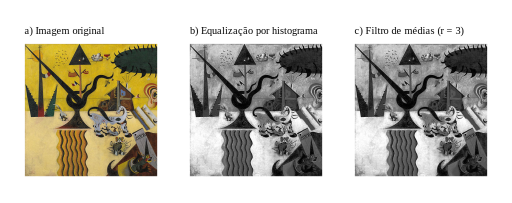
\includegraphics[scale=1.2]{figs/passos_eq}
     \fonteminha
\end{center}
\end{figure}

Algoritmos de extração de características foram aplicados a versões
coloridas, em escala de cinza e preto-e-branco das imagens
(figura~\ref{fig:tipos}), conforme necessário. Por exemplo, para o algoritmo
\textit{convex-hull}, uma imagem binária foi utilizada, enquanto que para o
algoritmo de textura de Haralick, uma imagem em escala de cinza foi
utilizada, já a segmentação SLIC utilizou a versão RGB de cada
imagem.

\begin{figure}[ht!]
\begin{center}
         \caption{Tipos de imagens utilizadas no estudo. \textit{a)}
        imagem colorida em formato RGB, \textit{b)} imagem em
        escala de cinza, e \textit{c)} imagem bi\-ná\-ria.}
        \label{fig:tipos}
        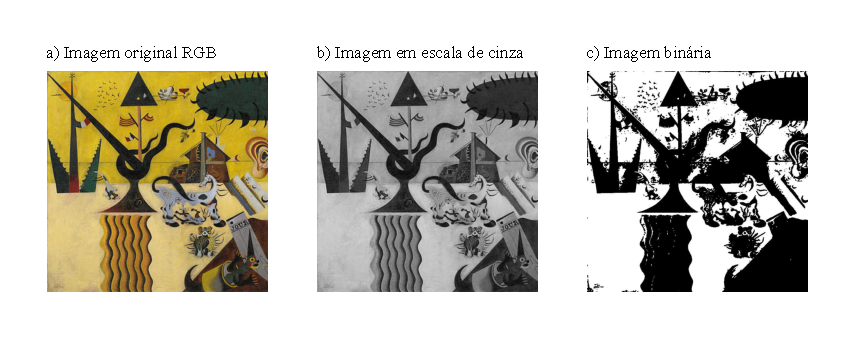
\includegraphics[scale=1.2]{figs/passos_tipos}
       \fonteminha
\end{center}
\end{figure}

Com o objetivo de mensurar características de regiões das pinturas,
métodos de segmentação foram utilizados, a saber: Watershed, SLIC e
Felzenswald.~\cite{gonzalez,luciano} Após experimentos
(figura~\ref{fig:expsegs}), preferiu-se o método de segmentação SLIC
(descrito na subseção~\ref{sec:slic}), por apresentar melhor separação
das regiões de cada pintura. O parâmetro $k$ (número
de \textit{clusters}) da segmentação SLIC foi ajustado de forma a
melhor segmentar as regiões. Como é possível notar no
detalhe \textit{e)} da figura~\ref{fig:expsegs}, valores de $k>10$
revelaram resultados que não contribuiriam para a segmentação
desejada.

\begin{figure}[h!]
\begin{center}
         \caption{Experimentos realizados para segmentação de
        pinturas, considerando ambas pinturas barrocas e
        modernas. \textit{a)} a imagem original, \textit{b)}
        segmentação por Watershed, \textit{c)}
        Felzenswald, \textit{d)} SLIC com $k=10$ e \textit{e)} SLIC
        com $k=20$. O método SLIC com $k=10$ foi escolhido por apresentar,
        visualmente, melhor separação dos segmentos, e os parâmetros
        escolhidos contribuíram para a seg\-men\-ta\-ção
        apresentada.}  \label{fig:expsegs} 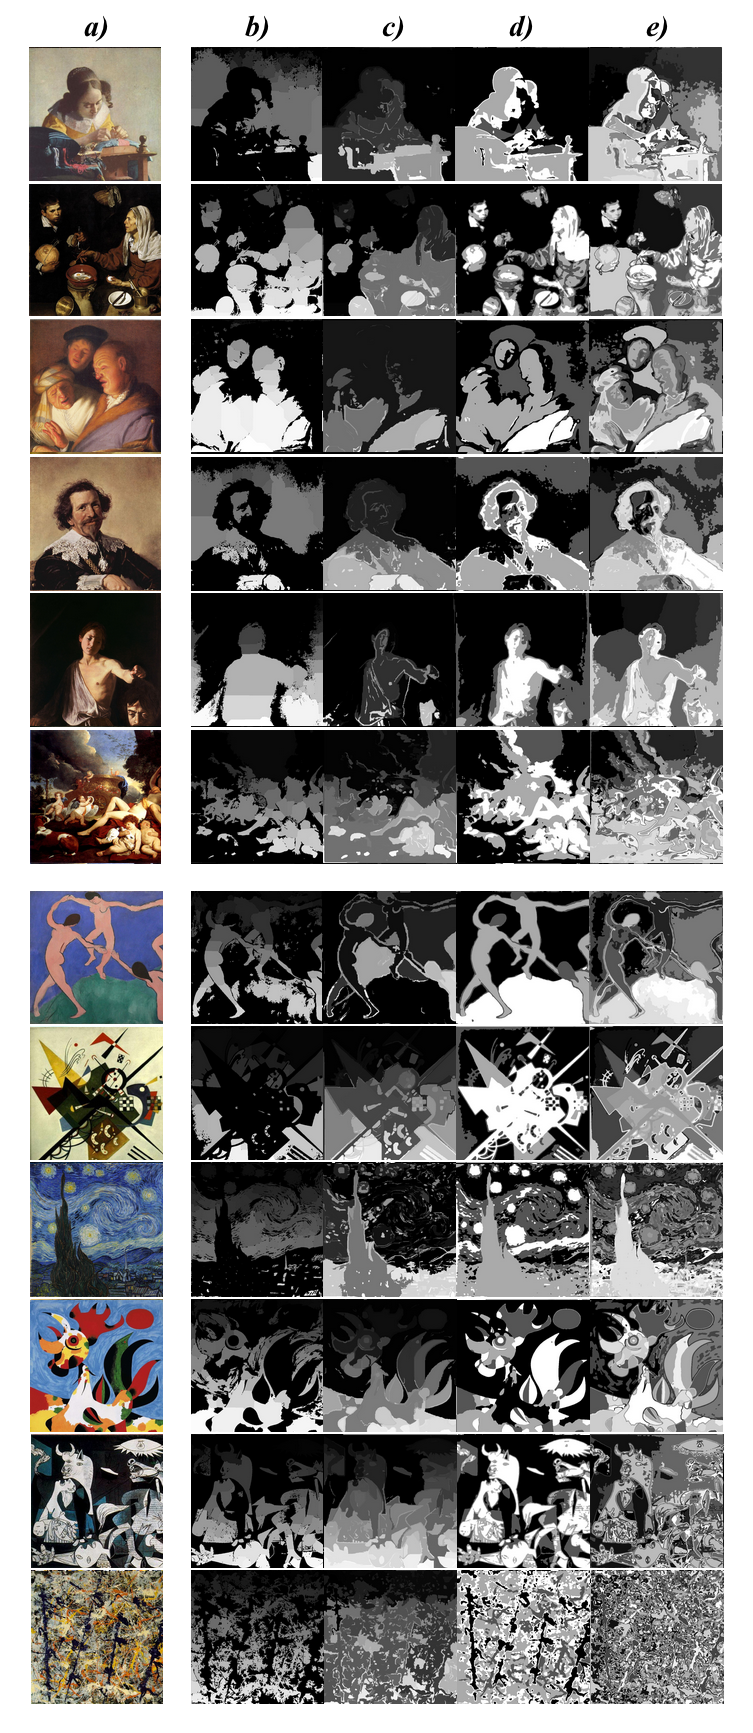
\includegraphics[scale=.3]{figs/expsegs} \fonteminha
\end{center}
\end{figure}

Tendo-se as regiões segmentadas, estas foram rotuladas em objetos
conexos, ou seja, em regiões conectadas e independentes umas das
outras. Os objetos conexos com área menor que um dado limiar (definido experimentalmente) foram removidos da imagem, como mostra a figura~\ref{fig:rotulacao}. Após esta etapa de pós-processamento, partiu-se
para o cálculo de curvatura de cada região e demais atributos descritos
na seção~\ref{sec:atributos}. A figura~\ref{fig:passos_curvatura} mostra algumas das regiões segmentadas e suas respectivas curvaturas. É possível notar que o cálculo da curvatura consegue identificar os picos de curvatura (marcados em vermelho) da maneira esperada.

\begin{figure}[h!]
\begin{center}
          \caption{Pós-processamento através da rotulação dos componentes
        conexos e sua filtragem, removendo as regiões com áreas
        menores que um dado limiar. \textit{a)} Detalhe de regiões
        segmentadas através do algoritmo SLIC, \textit{b)} objetos
        rotulados, \textit{c)} objetos com área menor que limiar
        removidos. É a partir desta última imagem que se realizou a
        extração de características.}
        \label{fig:rotulacao}
        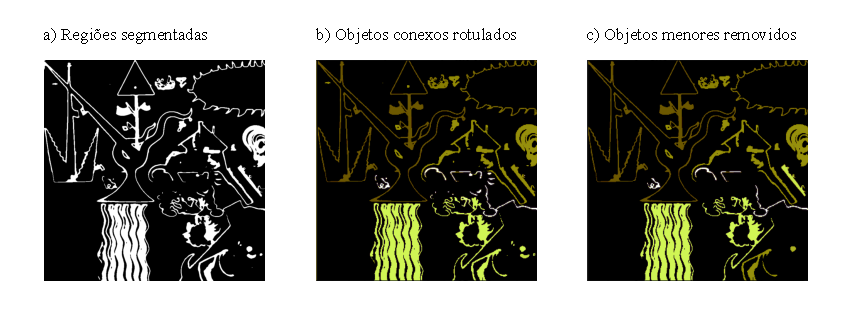
\includegraphics[scale=1.2]{figs/passos_rotulacao}
        \fonteminha
\end{center}
\end{figure}

\begin{figure}[h!]
\begin{center}
            \caption{Regiões segmentadas e suas respectivas
        curvaturas. Os marcadores em vermelho identificam os picos de
        curvatura no perfil e sua localização na região segmentada. O
        cálculo de curvatura demonstra desempenho esperado na
        identificação dos picos de
        curvatura.}  \label{fig:passos_curvatura} 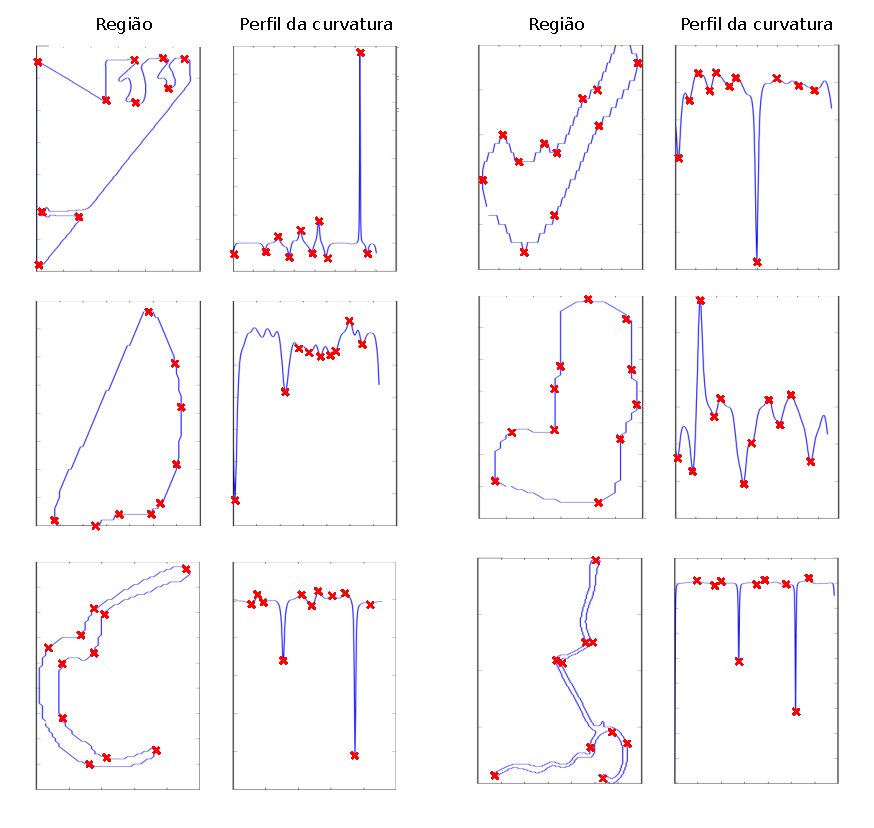
\includegraphics[scale=1]{figs/passos_curvatura} \fonteminha
\end{center}
\end{figure}

Todo o processo está representado esquematicamente na figura~\ref{fig:dataflow}
e abrange todos os passos, do processamento das pinturas até o
cálculo das medidas de dialética, oposição e inovação, discutidas em detalhes nas
próximos seções, e portanto, destacadas na figura.

\begin{figure}[h!]
\begin{center} 
          \caption{Diagrama com todos os passos tomados, desde o processamento das
        imagens das pinturas até a extração de características, assim como a
        obtenção da série temporal onde foram calculadas as medidas de oposição,
        inovação e dialética.}
        \label{fig:dataflow}
        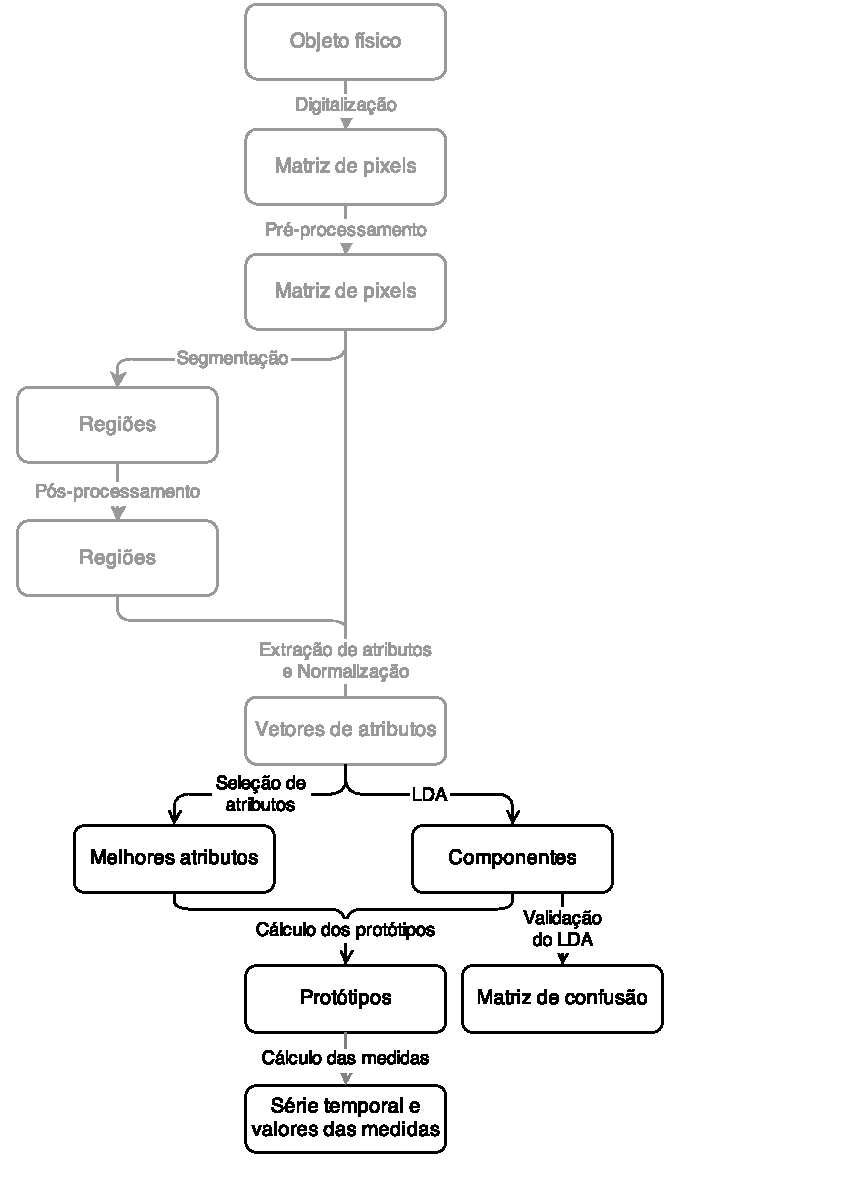
\includegraphics[scale=.8]{figs/dataflow_pintores3}
        \fonteminha
\end{center}
\end{figure}
\clearpage
\section{Seleção de atributos}

Para selecionar os atributos mais relevantes, neste caso, os atributos
que separassem melhor os grupos de pinturas --- em outras palavras,
que garantissem menor covariância interna em cada classe e maior
covariância entre as classes --- uma medida de dispersão foi aplicada
usando as matrizes de espalhamento discutidas na
seção~\ref{sec:fund:reducao}.

Calculando $\alpha$ através da eq.~\ref{eq:alpha} para todos os
possíveis pares de atributos $F_{N, a}$ e $F_{N, b}$ dos $N = 100$
atributos e ordenando os resultados por $\alpha$, é possível
selecionar os atributos mais relevantes para a classificação.
Pares com maiores valores de $\alpha$ apresentam melhor dispersão
interclasse e agrupamento intraclasse do que pares com menores
valores. Como visto na tabela~\ref{tab:alpha} (e mais a frente, nas
figuras~\ref{fig:caso1_g1} e~\ref{fig:caso1_g2}), os atributos
\emph{média dos picos de curvatura} e \emph{média do número de
  segmentos} possuem maior valor de $\alpha$ e foram selecionados para
a análise das medidas de oposição, inovação e dialética --- ambos
atributos se mostraram predominantes mesmo na projeção por LDA,
discutida na seção~\ref{subsec:lda}. É interessante notar a natureza
dos atributos selecionados: o \textit{número de segmentos em cada pintura} e os
\textit{picos de curvatura} são características proeminentes para a
classificação das pinturas, melhores até mesmo que os atributos de
textura de Haralick e de complexidade de imagens (i.e.\
entropia). Outros atributos que apresentaram valores altos de $\alpha$
são também relacionados com características de forma, como:
\textit{média da área de convex-hull}, \textit{média do perímetro dos segmentos}, \textit{média da área dos segmentos}, e \textit{circularidade}. Estes atributos apresentaram projeções e
propriedades de agrupamento similares às da figura~\ref{fig:caso1_g1}
como mostrado na figura~\ref{fig:scatters}.
 
\begin{table}[ht] \footnotesize
  \begin{center}
  \caption{\label{tab:alpha} Pares de atributos $F_{N, a}$ e $F_{N, b}$
    ordenados por
    $\alpha$. Pares com valores maiores de $\alpha$ mostram maior dispersão
    interclasse enquanto menor dispersão intraclasse (maior agrupamento).
    O melhor par de atributos: \emph{média dos picos de curvatura} e
    \emph{média do número de segmentos} foram selecionados para a análise e
    cálculo das medidas de oposição, inovação e dialética.}
\begin{tabular}{@{}llll}
 \hline \hline
 \textbf{Par} & \textbf{Atributo $a$}    & \textbf{Atributo $b$}   & \textbf{$\alpha$} \\ 
 
 \hline
 
 1 & média do número de picos & média do número de segmentos & 42.445 \\
 2 & média do número de segmentos & média da área de convex-hull & 37.406 \\
 3 & média do perímetro do segmento & média do número de segmentos & 36.703 \\
 4 & média da área do segmento & média do número de segmentos & 36.214 \\
 5 & média do número de segmentos & média área convexa / área total & 34.885 \\
 6 & média de circularidade ($\mathrm{Per.}^2/\mathrm{Area}$) & média do número
 de segmentos & 33.540 \\
 7 & média da energia das linhas (canal verde) & média do número de segmentos & 32.954 \\
 8 & média da energia das linhas e colunas (canal verde) & média do número de segmentos & 32.954 \\
 9 & d.p. da energia das linhas (canal verde) & média do número de segmentos & 32.932 \\
 10 & d.p. da energia das linhas e colunas (canal verde) & média do número
 de segmentos & 32.906 \\
 11 & média de entropia local (janela de dimensão 5) & média do número de segmentos & 32.898 \\
 12 & entropia (Haralick adj. 4) & média do número de segmentos & 32.898 \\
 13 & entropia (Haralick adj. 3) & média do número de segmentos & 32.883 \\
 14 & entropia (Haralick adj. 1) & média do número de segmentos & 32.874 \\
 15 & entropia (Haralick adj. 2) & média do número de segmentos & 32.869 \\
 16 & média da energia das linhas (canal vermelho) & média do número de segmentos & 32.865 \\
\hline \hline
 \end{tabular}
 \fonteminha
\end{center}
\end{table}

\begin{figure}[h!]
\begin{center}
      \caption{Matrizes de espalhamento para cada $i$-ézimo par de atributos, listadas na
        tabela~\ref{tab:alpha} em ordem decrescente de $\alpha$. A primeira
        projeção (par $1$) foi utilizada nesse estudo.}
        \label{fig:scatters}
        \end{center}
{    \centering
        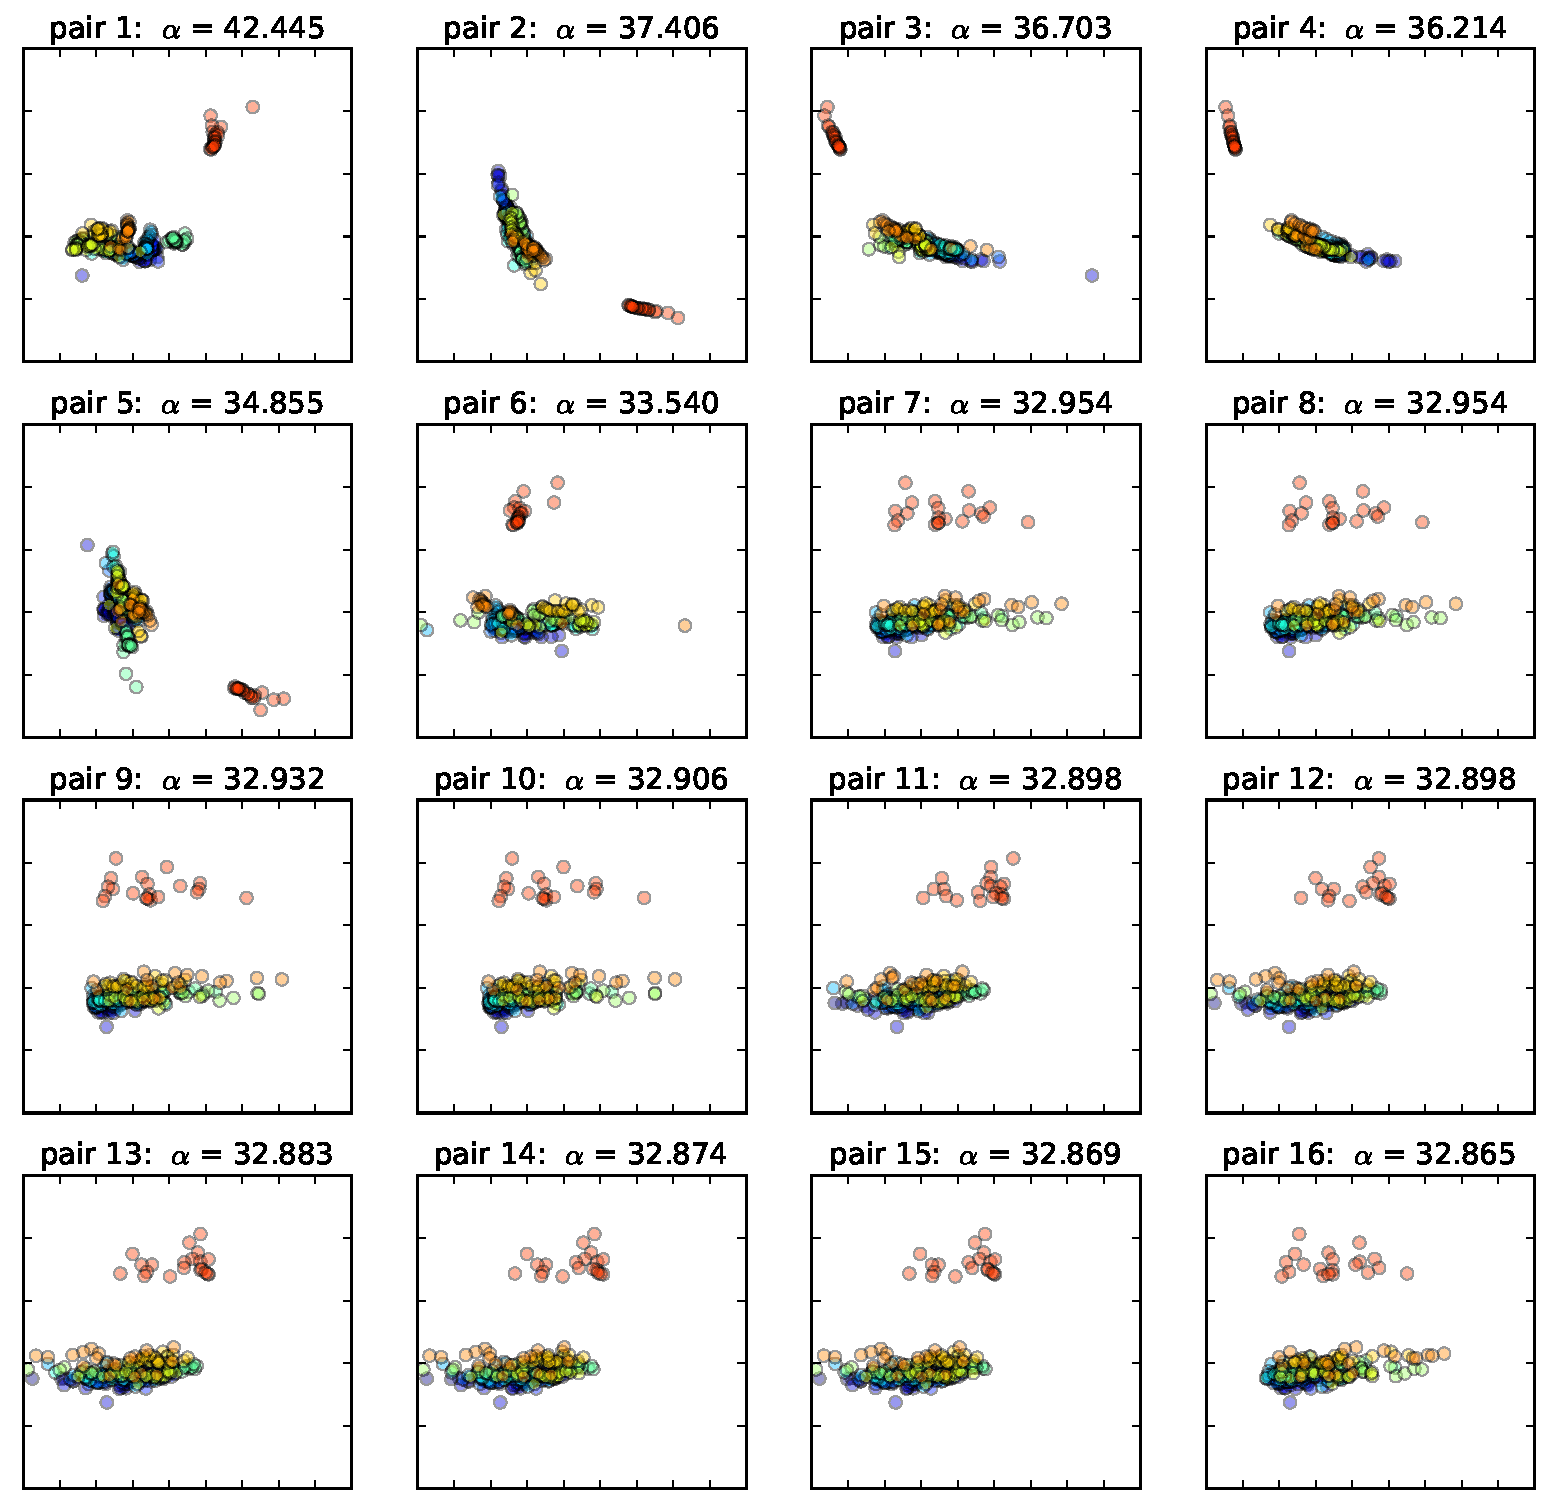
\includegraphics[width=\columnwidth]{figs/sm_pintores}}
        \fonteminha
\end{figure}

\clearpage
\section{Medidas de dialética, oposição e inovação}
\label{sec:medidas}

Havendo $N_f$ atributos $\vec{f_i}$, define-se um espaço
$N_f$-dimensional chamado de \textit{espaço criativo}, pois a exemplo
do espaço criativo sugerido por Deleuze,~\cite{deleuze} tem como
objetivo a representação de uma superfície onde artefatos
(e.g.\ pinturas, peças musicais ou poemas) criados por agentes
(e.g.\ pintores, compositores ou escritores) caracterizam uma região que
foi explorada criativamente. É neste espaço criativo que as medidas de
dialética, oposição e inovação são calculadas.~\cite{vieira}

Para simplificar o cálculo, um protótipo $\vec{p_i}$ é definido para cada classe
$C_p$. Cada protótipo sumariza uma classe de pinturas (ou um pintor),
correspondendo ao seu \textit{centroide}: $\vec{p_i} = \frac{1}{N_p}
\sum_{i=1}^{N_p} \vec{f_i}$ calculado no espaço projetado. É importante notar
que essa medida é independente de dimensão, porém métodos de redução de
dimensionalidade são aplicados à matriz de atributos para possibilitar a
visualização do \textit{espaço criativo} em duas dimensões.

Uma sequência $S$ de $\vec{p_i}$ estados define uma série temporal que
modela uma aproximação do que seria a linha cronológica para as
pinturas e seus movimentos artísticos. Um estado médio em um dado
tempo $i$ abrangendo os estados $\vec{p_1}$ até $\vec{p_i}$ é definido
como

\begin{equation}
\vec{a_i} = \frac{1}{i}\sum_{j=1}^i\vec{p}_j.
\end{equation}

O estado de oposição $\vec{r_i}$ define uma medida de oposição à $\vec{p_i}$ como

\begin{equation}
\vec{r}_i = \vec{p}_i + 2(\vec{a}_i - \vec{p}_i)
\end{equation}

\noindent e dessa forma, um vetor de oposição $\vec{D}_i$ pode ser definido como

\begin{equation}
\vec{D}_i=\vec{r}_i - \vec{p}_i
\end{equation}

\noindent que representa o deslocamento do estado $\vec{r}_i$ em
função de $\vec{p}_i$.

Sabendo que qualquer deslocamento a partir de um estado $\vec{p_i}$ até um outro
estado $\vec{p_j}$ é definido como

\begin{equation}
\vec{M}_{i,j} = \vec{p}_j - \vec{p}_i
\end{equation}

\noindent é possível definir um \emph{índice de oposição} $W_{i,j}$ para
quantificar quanto um protótipo $\vec{p_j}$ se opõe a outro protótipo $\vec{p_i}$ (ou seja,
um deslocamento na direção de $\vec{r_i}$) ou concorda com outro protótipo $p_i$
(um deslocamento na direção de $-\vec{r_i}$):

\begin{equation}
W_{i,j} = \frac{\left< \vec{M}_{i,j}, \vec{D}_j\right>}{||\vec{D}_j||^2}
\end{equation}

\noindent sendo portanto a projeção de $\vec{M}_{i,j}$ em $\vec{D}_i$, ou seja,
não importa onde o deslocamento tenha se dado, ele é considerado em relação ao
vetor de oposição (ou deslocamento) $\vec{D}_i$. A
figura~\ref{fig:desc_opos_inov} ilustra $\vec{D}_i$, dados dois estados
consecutivos $\vec{p_i}$ e $\vec{p_j}$, o estado de oposição $\vec{r_i}$ e o
estado médio $\vec{a_i}$.

Porém, movimentos nesse \textit{espaço criativo} não estão restritos à
confirmação ou contradição de ``ideias''. Ideias alternativas podem existir fora
desse deslocamento dualístico. Isso é modelado como um \emph{índice de inovação}
que quantifica quanto um protótipo $\vec{p_j}$ é inovador quando comparado com um
outro protótipo $\vec{p_i}$:

%% Explicar em detalhes baseando-se em http://mathworld.wolfram.com/Point-LineDistance3-Dimensional.html

\begin{equation}
s_{i,j} = \sqrt{\frac{|\vec{p}_i-\vec{p}_j|^2
          |\vec{a}_i-\vec{p}_i|^2 - 
          [(\vec{p}_i-\vec{p}_j) . 
            (\vec{a}_i-\vec{p}_i)]^2}
        {|\vec{a}_i-\vec{p}_i|^2}}
\end{equation}

\noindent ou seja, quanto $\vec{p_j}$ se afasta da linha $L_i$ formada por $\vec{p_i}$ e
$\vec{r_i}$: a linha de ``oposição''.  A
figura~\ref{fig:desc_opos_inov} também ilustra os cálculos dos índices
de oposição e inovação para dois estados consecutivos $\vec{p_i}$ e
$\vec{p_j}$ da série temporal e uma linha $L_i$.

\begin{figure}[ht!]
\begin{center}
              \caption{Cálculo dos índices de oposição $W_{i,j}$ --- com base
        no deslocamento $\vec{D_j}$ e inovação $s_{i,j}$ dados dois
        estados consecutivos $\vec{p_i}$ e $\vec{p_j}$.}
        \label{fig:desc_opos_inov}
        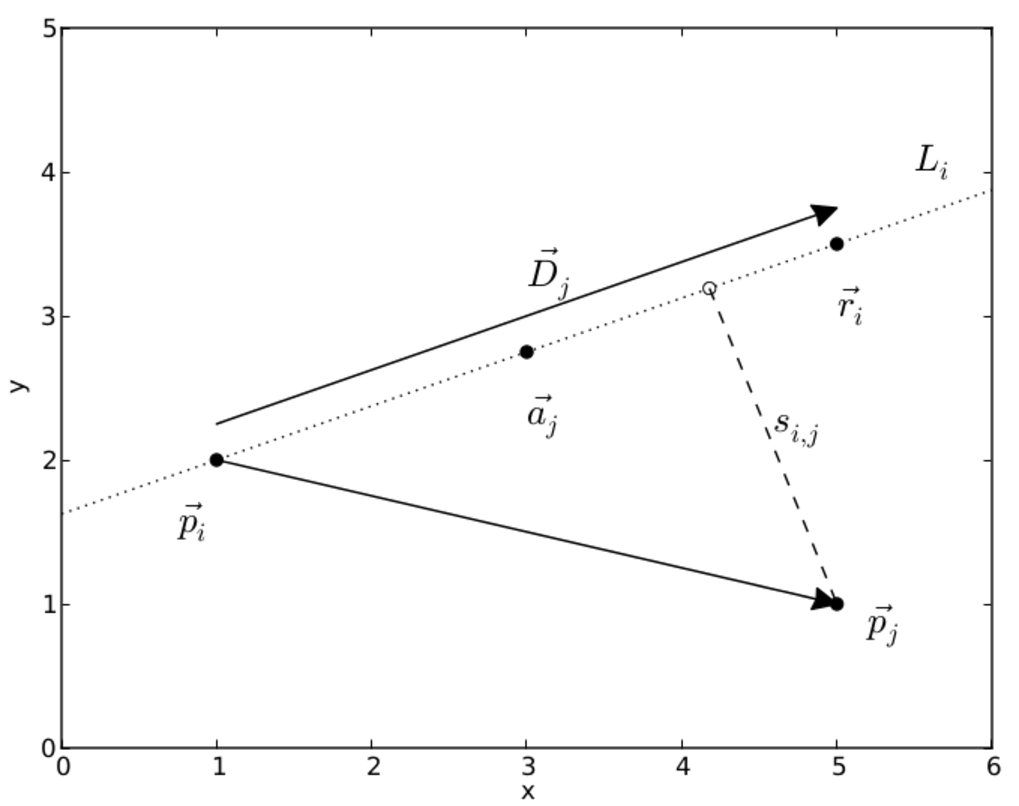
\includegraphics[scale=.6]{figs/desc_opos2.pdf}
        \fonteminha
\end{center}
\end{figure}

Uma outra medida surge quando consideram-se três estados consecutivos
nos tempos $i, j$ e $k$. Sendo $\vec{p_i}$ a tese, $\vec{p_j}$ a
antítese e $\vec{p_k}$ a síntese, um \emph{índice de
  contra-dialética}~\cite{vieira} pode ser definido como

%% TODO: deduzir como uma generalização de http://mathworld.wolfram.com/Point-PlaneDistance.html

\begin{equation}
d_{i \rightarrow k} = 
      \frac{|\left< \vec{p}_j-\vec{p}_i,\vec{p}_k \right> + 
        \frac{1}{2}\left<\vec{p}_i-\vec{p}_j, \vec{p}_i+\vec{p}_j\right>|}
           {|\vec{p}_j-\vec{p}_i|}
\end{equation}

\noindent ou, a distância entre $\vec{p_k}$ e a mediatriz $B_{i,j}$
(ou um ``hiperplano mediatriz'' quando considerando espaços
$N_f$-dimensionais com $N_f>3$) entre $\vec{p_i}$ e $\vec{p_j}$. Em
outras palavras, um estado $\vec{p_k}$ com grande distância $d_{i
  \rightarrow k}$ está afastado da síntese (possui baixa dialética) e
vice-versa. A medida de contra-dialética $d_{i \rightarrow k}$ é
ilustrada na figura~\ref{fig:desc_dialetica} para três estados
consecutivos $\vec{p_i}$, $\vec{p_j}$ e $\vec{p_k}$ da série temporal,
dada uma mediatriz $B_{i,j}$ formada pelos dois primeiros estados da
série.

\begin{figure}[ht!]
\begin{center}
      \caption{Cálculo da contra-dialética $d_{i \rightarrow k}$ dados os
        estados consecutivos de tese $\vec{p_i}$, antítese $\vec{p_j}$ e síntese
        $\vec{p_k}$. Quanto maior o valor da distância $d_{i \rightarrow k}$ de
        $\vec{p_k}$ à síntese ideal formada pela mediatriz $B_{i,j}$ entre
        $\vec{p_i}$ e $\vec{p_j}$, menor a dialética.  }
        \label{fig:desc_dialetica}
        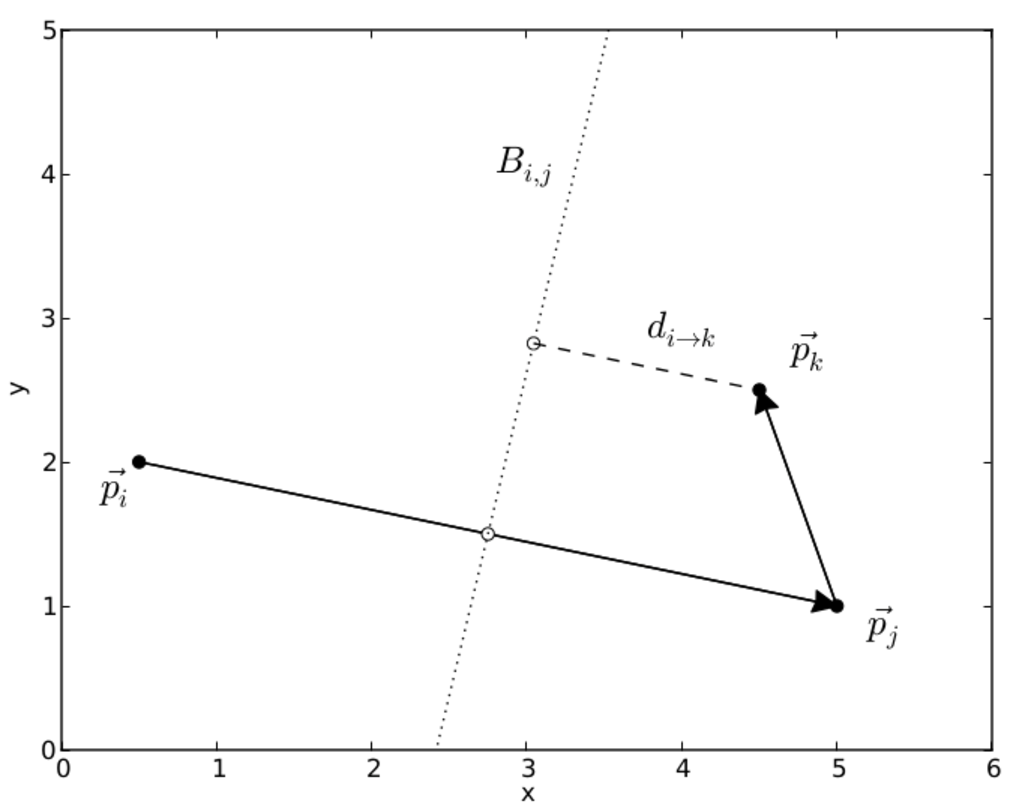
\includegraphics[scale=.6]{figs/desc_dialetica2.pdf}
      \fonteminha
\end{center}
\end{figure}

%%%%%
\clearpage
\section{Análise das pinturas para atributos com maior dispersão}
\label{sec:pares}

O \textit{espaço criativo} considerando todas as pinturas
``representadas'' por $\vec{p_i}$ e tendo como bases os
atributos \emph{média de picos da curvatura} e \emph{média do número
de segmentos} é apresentado na figura~\ref{fig:caso1_g1}. A série
temporal formada pelos protótipos $\vec{p_i}$ para cada pintor no
espaço projetado é visto na figura~\ref{fig:caso1_g2}, facilitando a
visualização da evolução da série.

% gerado com: metrics_caso1.py
\begin{figure}[h!]
\begin{center}
           \caption{Projeção do \textit{espaço criativo} considerando o
        melhor par de atributos \emph{média de picos da curvatura} e
        \emph{média do número de segmentos}.}
        \label{fig:caso1_g1}
        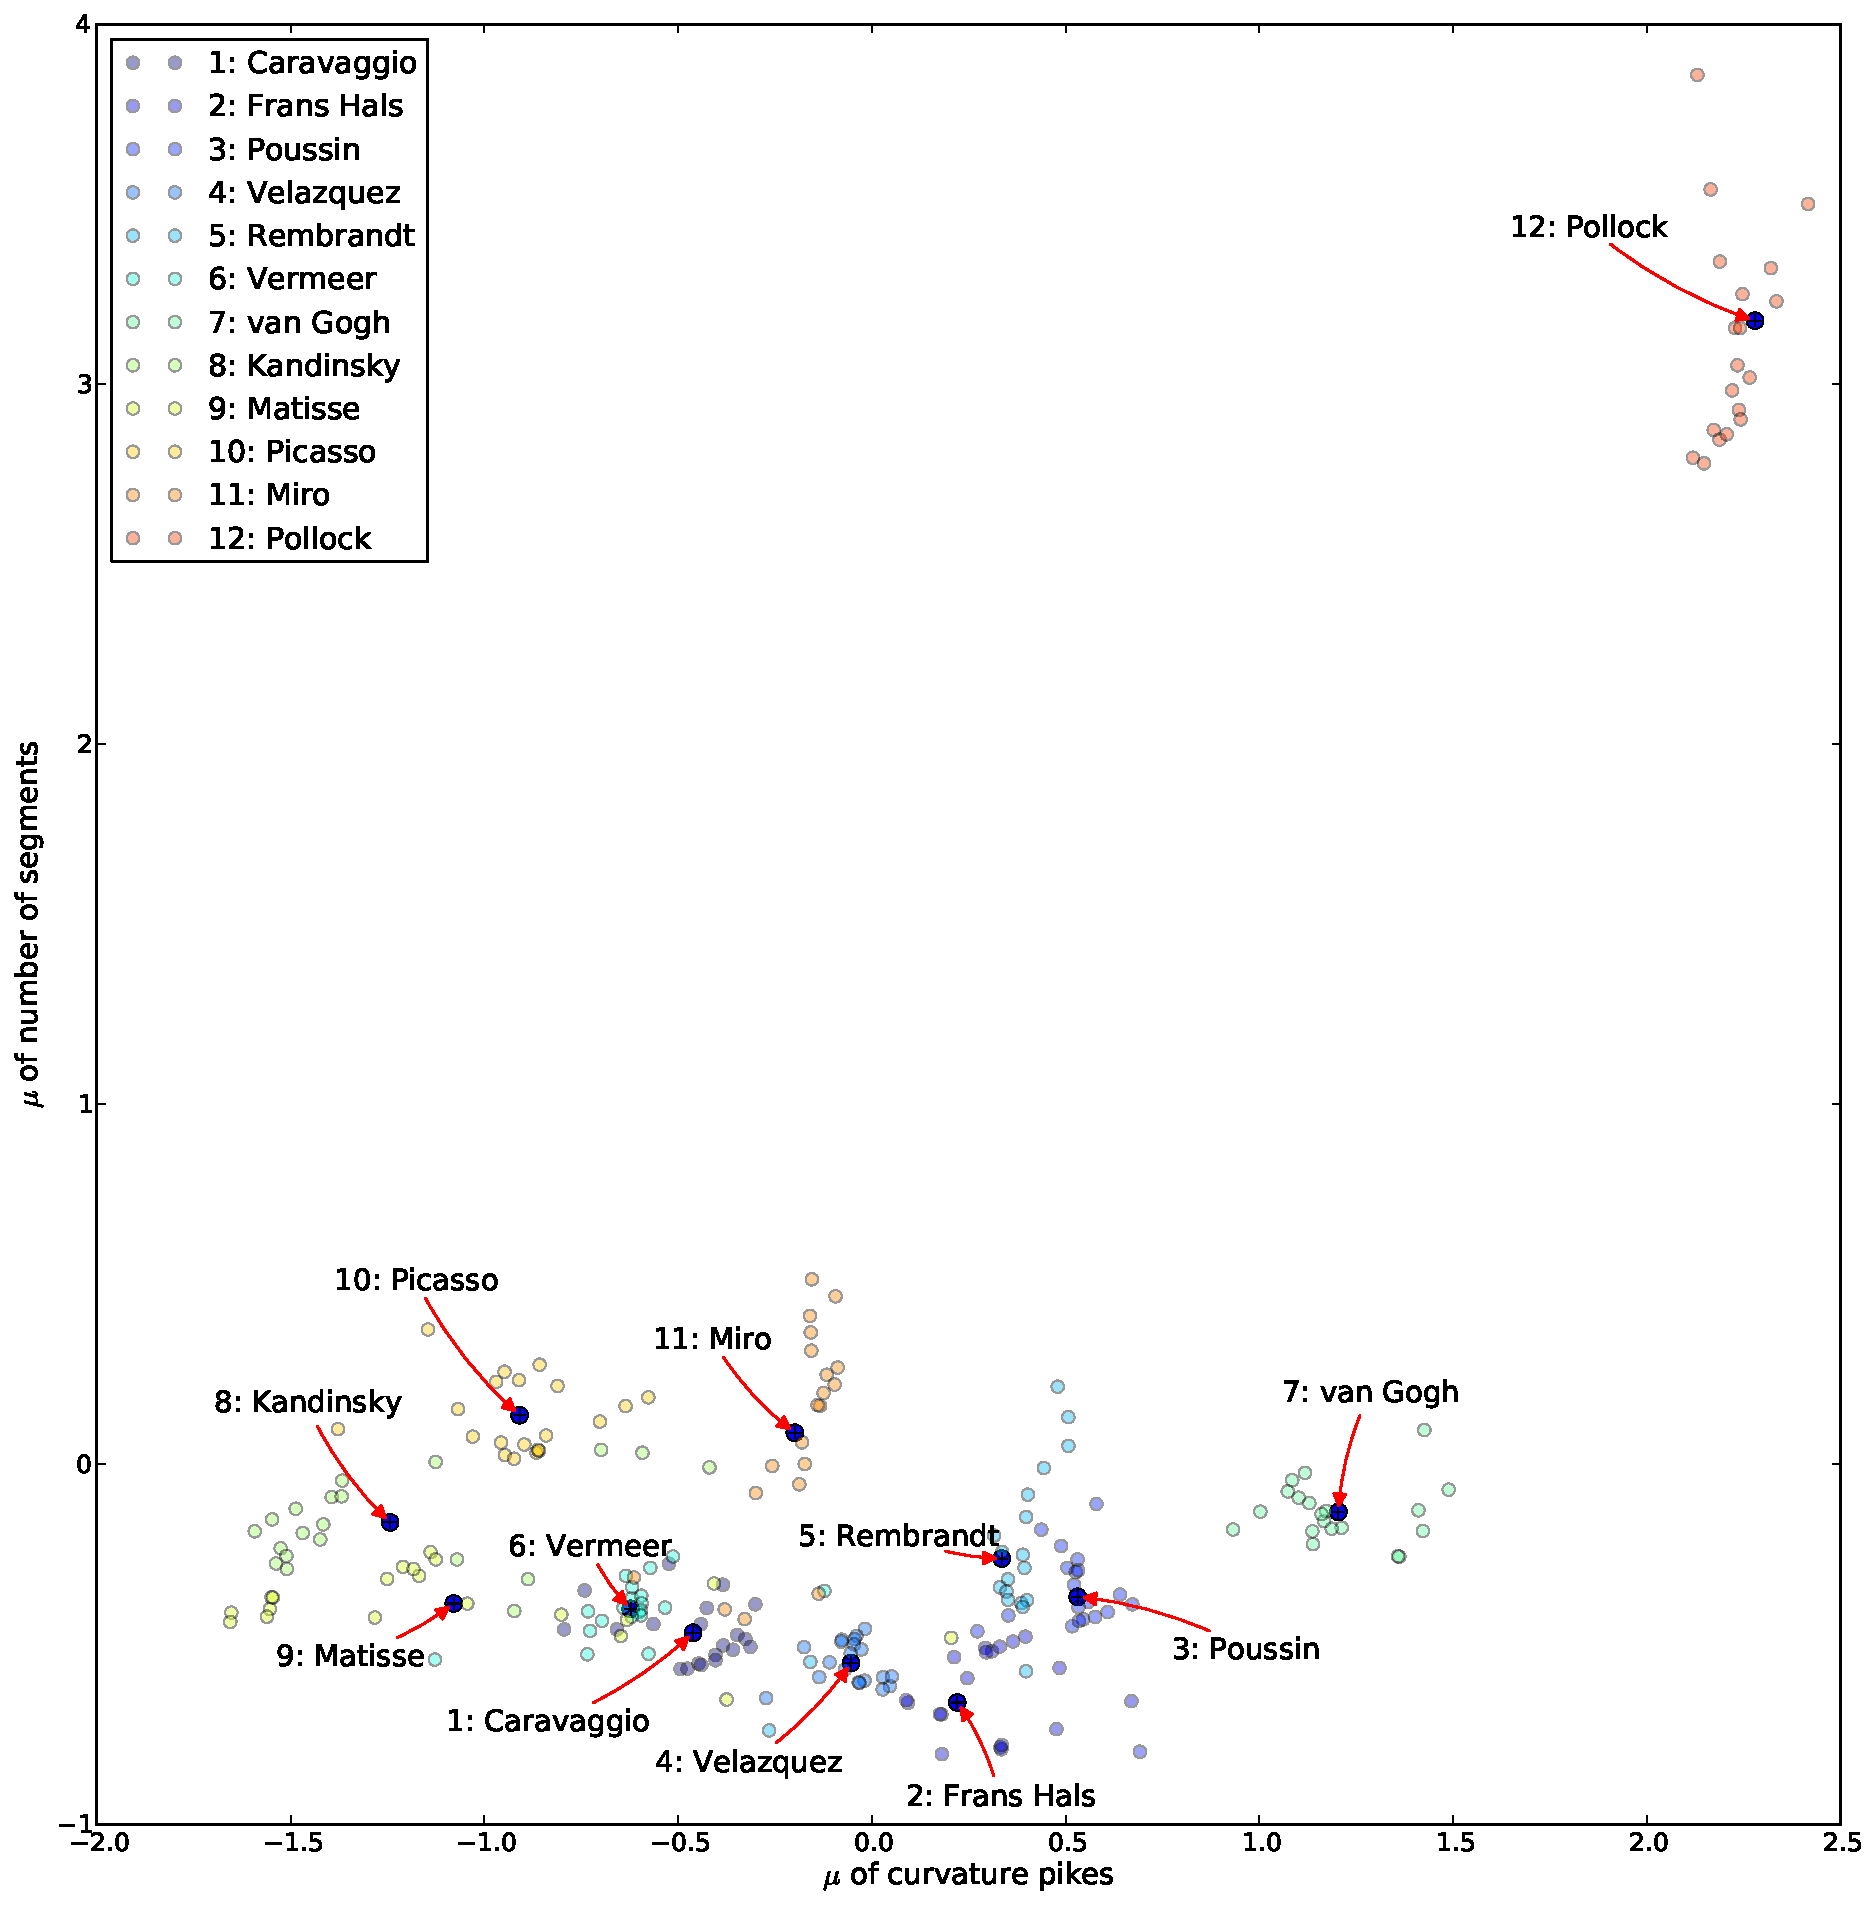
\includegraphics[scale=.5]{figs/caso1_g1}
        \fonteminha
\end{center}
\end{figure}

% gerado com: metrics_caso1.py
\begin{figure}[h!]
\begin{center}
         \caption{Série temporal considerando o melhor par de atributos
        \emph{média de picos da curvatura} e \emph{média do número de
          segmentos}.}
        \label{fig:caso1_g2}
        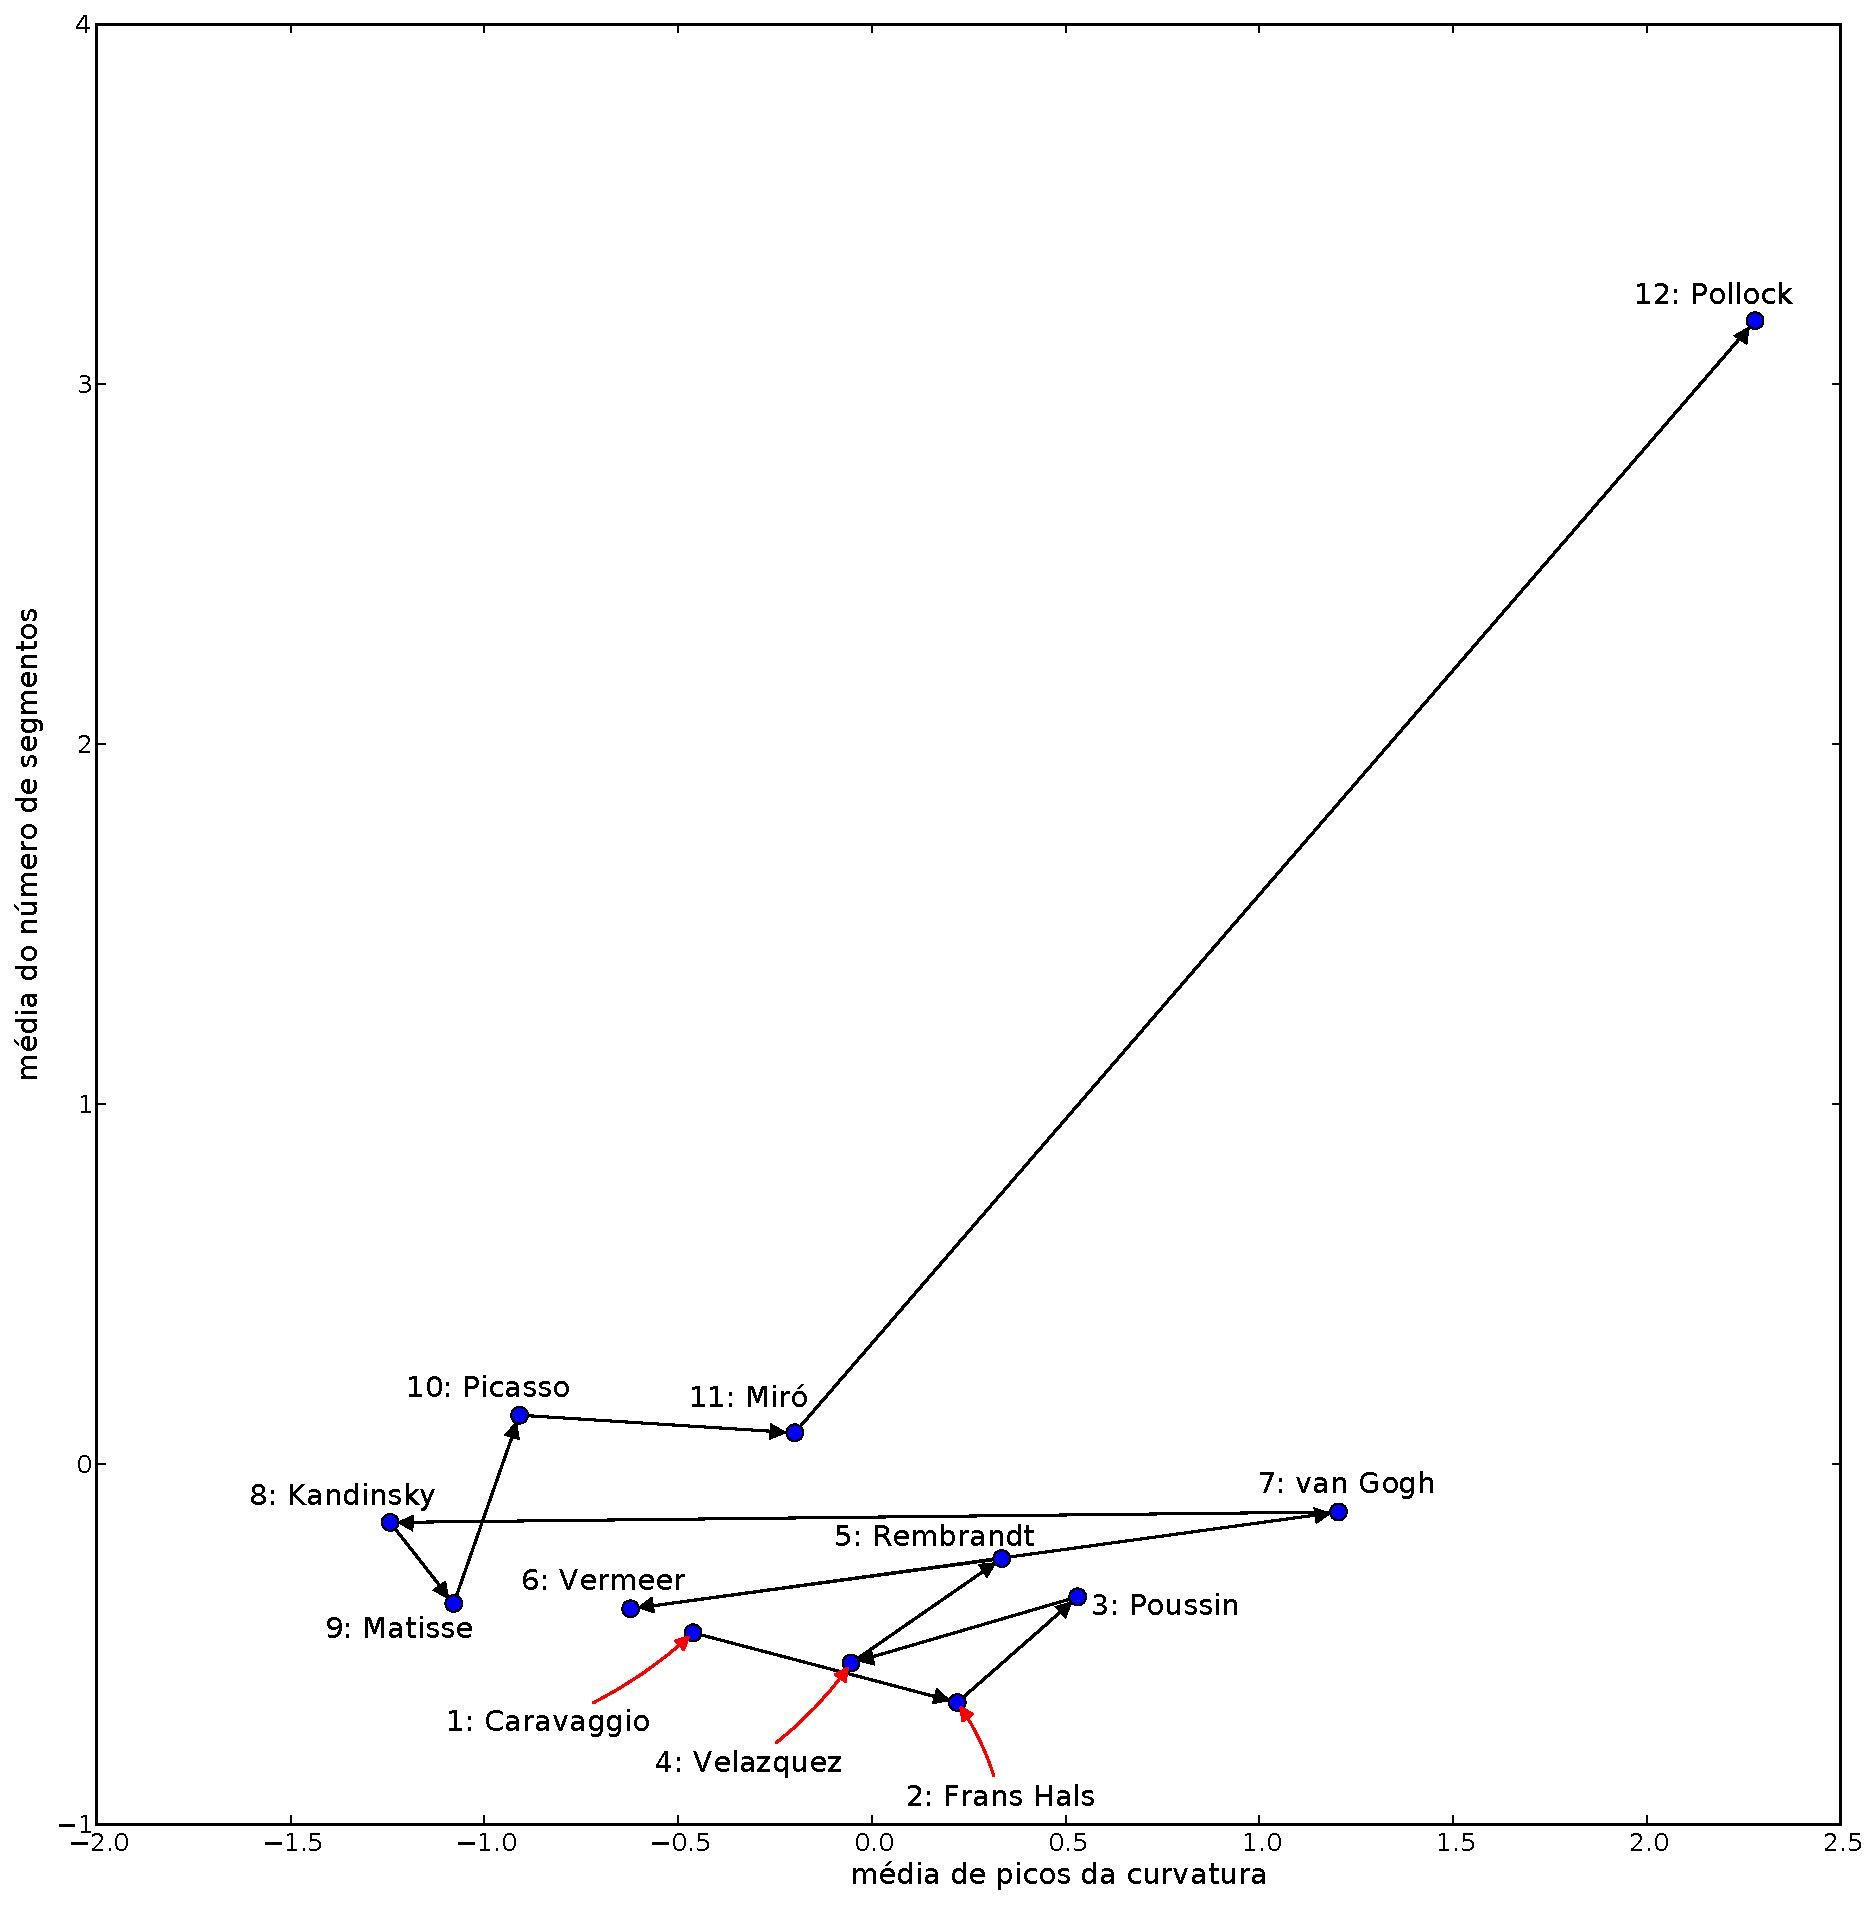
\includegraphics[scale=.5]{figs/caso1_g2}
        \fonteminha
\end{center}
\end{figure}

Detalhes interessantes surgem dessa projeção e confirmam
algumas das hipóteses levantadas na seção~\ref{subsec:sumario}, aqui
relembradas e confrontadas com interpretações a partir dos dados
quantitativos obtidos na projeção:

\begin{itemize}
  \item \textit{Os pintores da Arte Moderna são caracterizados por sua
    independência em estilo. Já os pintores do período Barroco
    apresentam semelhanças, por compartilharem estilos tradicionais.}
    Essa é uma das observações mais relevantes deste estudo. É
    possível notar na figura~\ref{fig:caso1_g1} que há maior
    sobreposição entre pintores barrocos do que pintores dos
    movimentos modernos. Esse fato é confirmado pela história da Arte,
    onde os pintores modernos experimentam novos materiais e
    desenvolvem estilos próprios,
    enquanto os barrocos tendem a utilizar estilos tradicionais, como
    o \textit{chiaroscuro} de Caravaggio. Os deslocamentos de um
    artista ao outro também são claramente contrastantes: o módulo dos
    vetores de deslocamento $\vec{M}_{i,j}$ para os pintores modernos
    é, em média, maior que os deslocamentos para os pintores
    barrocos. Este é mais um indicador de que os artistas barrocos
    compartilhavam semelhanças em estilo, enquanto que os modernos
    distanciavam-se claramente uns dos outros. Ao contemplar a
    figura~\ref{fig:caso1_g2} percebe-se que há uma certa exploração
    do que seria o \textit{espaço criativo} por parte dos artistas
    barrocos, mas a largura dessa exploração não se compara à
    realizada pelos pintores modernos que percorrem uma região muito
    mais ampla, chegando a explorar regiões de extremos opostos como
    no caso de Pollock.

\item \textit{Há uma diferença cronológica considerável entre o
  Barroco e os movimentos da Arte Moderna}. Quando se observa a
  série temporal da figura~\ref{fig:caso1_g2}, a diferença entre os
  períodos fica evidente: enquanto os barrocos retornam uns aos
  outros, há um deslocamento abrupto em Van Gogh --- o primeiro pintor
  moderno considerado nesse estudo --- que o separa dos primeiros
  pintores. Van Gogh, embora localizado próximo aos pintores barrocos
  e no extremo oposto da maioria dos pintores modernos, estabelece o
  início do período Moderno e depois dele os deslocamentos de um vetor
  ao outro continuam a evoluir até alcançar seu ápice, em Pollock. Essa
  mesma separação entre os períodos Barroco e da Arte Moderna é
  notada nas medidas de dialética, oposição e inovação, discutidas
  mais à frente.

  \item \textit{Pollock apresenta pinturas que diferem de todos os
    outros pintores escolhidos.} De todos os \textit{clusters} da
    projeção na figura~\ref{fig:caso1_g1}, Pollock é quem mais se
    distancia dos demais pintores. Isso se deve ao grande número de
    segmentos presentes nas pinturas de Pollock quando comparado aos
    demais artistas: o eixo-$y$ corresponde à projeção do atributo
    \emph{média do número de segmentos}. De qualquer forma, ambos
    eixos $x$ (\emph{média do número de picos da curvatura}) e $y$ são
    relevantes para separar os períodos Barroco e Moderno.

  \item \textit{Velázquez e Vermeer se assemelham com Caravaggio pois
    ambos utilizavam \textit{chiaroscuro}}. A trajetória desenhada (na
    figura~\ref{fig:caso1_g2}) de Caravaggio e Frans Hals até Poussin
    estabelece um caminho que termina com um movimento de oposição de
    Velázquez, que retorna a Caravaggio. Esse retorno a Caravaggio
    é também notado em Vermeer. Alguns críticos~\cite{lambert} sugerem
    que pintores como Vermeer nem teriam existido se não fosse a
    influência de Caravaggio: os agrupamentos de pinturas de Vermeer e
    Caravaggio apresentam a maior sobreposição dentre todos os
    agrupamentos presentes no \textit{espaço criativo}. Isso pode ser
    atribuído à influência do mestre do \textit{chiaroscuro} em ambos
    pintores, principalmente em Velázquez que foi reconhecidamente
    um estudioso das pinturas de Caravaggio.~\cite{gombrich} Ambos
    fatos são confirmados pelos histogramas do nível médio de cinza
    das pinturas, mostrados na figura~\ref{fig:chiaroscuro}. Os
    histogramas de Velázquez e Vermeer são os que mais se aproximam do
    histograma de Caravaggio quando comparados aos outros pintores
    barrocos. Nota-se que os histogramas de Rembrandt e Frans Hals
    também assemelham-se ao de Caravaggio, e estes pintores também
    utilizavam o \textit{chiaroscuro}. O histograma de Poussin é mais
    bem distribuído, refletindo suas pinturas mais claras, opondo-se à
    Caravaggio.

    \item \textit{Caravaggio é expoente no uso da técnica
      do \textit{chiaroscuro}.} Além da influência de Caravaggio em
      pintores como Velázquez e Vermeer, isso é também confirmado
      quando se comparam os histogramas dos pintores modernos na
      figura~\ref{fig:chiaroscuro_modernos} com os histogramas para os
      pintores barrocos da figura~\ref{fig:chiaroscuro}: há baixa
      similaridade entre os pintores modernos considerados,
      contrastando diretamente com os pintores barrocos, onde as
      curvas do histograma tendem à Caravaggio. Assim, afirma-se que há grande
      diferença de contraste entre as pinturas barrocas
      (principalmente as de Caravaggio) e aquelas da Arte Moderna.

    \item \textit{Poussin se opõe à Caravaggio: ele não deseja
retratar a verdade, mas sim o belo.} Poussin é o pintor que mais se
distancia do grupo barroco e também compreende o grupo de pinturas com
menor sobreposição, visível na figura~\ref{fig:caso1_g1}. É também o
pintor barroco que mais se distancia de Caravaggio segundo o valor de
$|\vec{M}_{i,j}|$ na projeção apresentada na
figura~\ref{fig:caso1_g2}.

\end{itemize}

\begin{figure}[h!]
\begin{center}
      \caption{Histogramas dos níveis médios de cinza para todos os
        pintores barrocos. Vermeer e Velázquez mostram maior
        similaridade com Caravaggio do que os outros pintores
        barrocos: a proximidade em contraste encontra fundamento na
        história (seção~\ref{subsec:sumario}), tendo sido ambos
        pintores influenciados por
        Caravaggio.}  \label{fig:chiaroscuro}
        { \centering 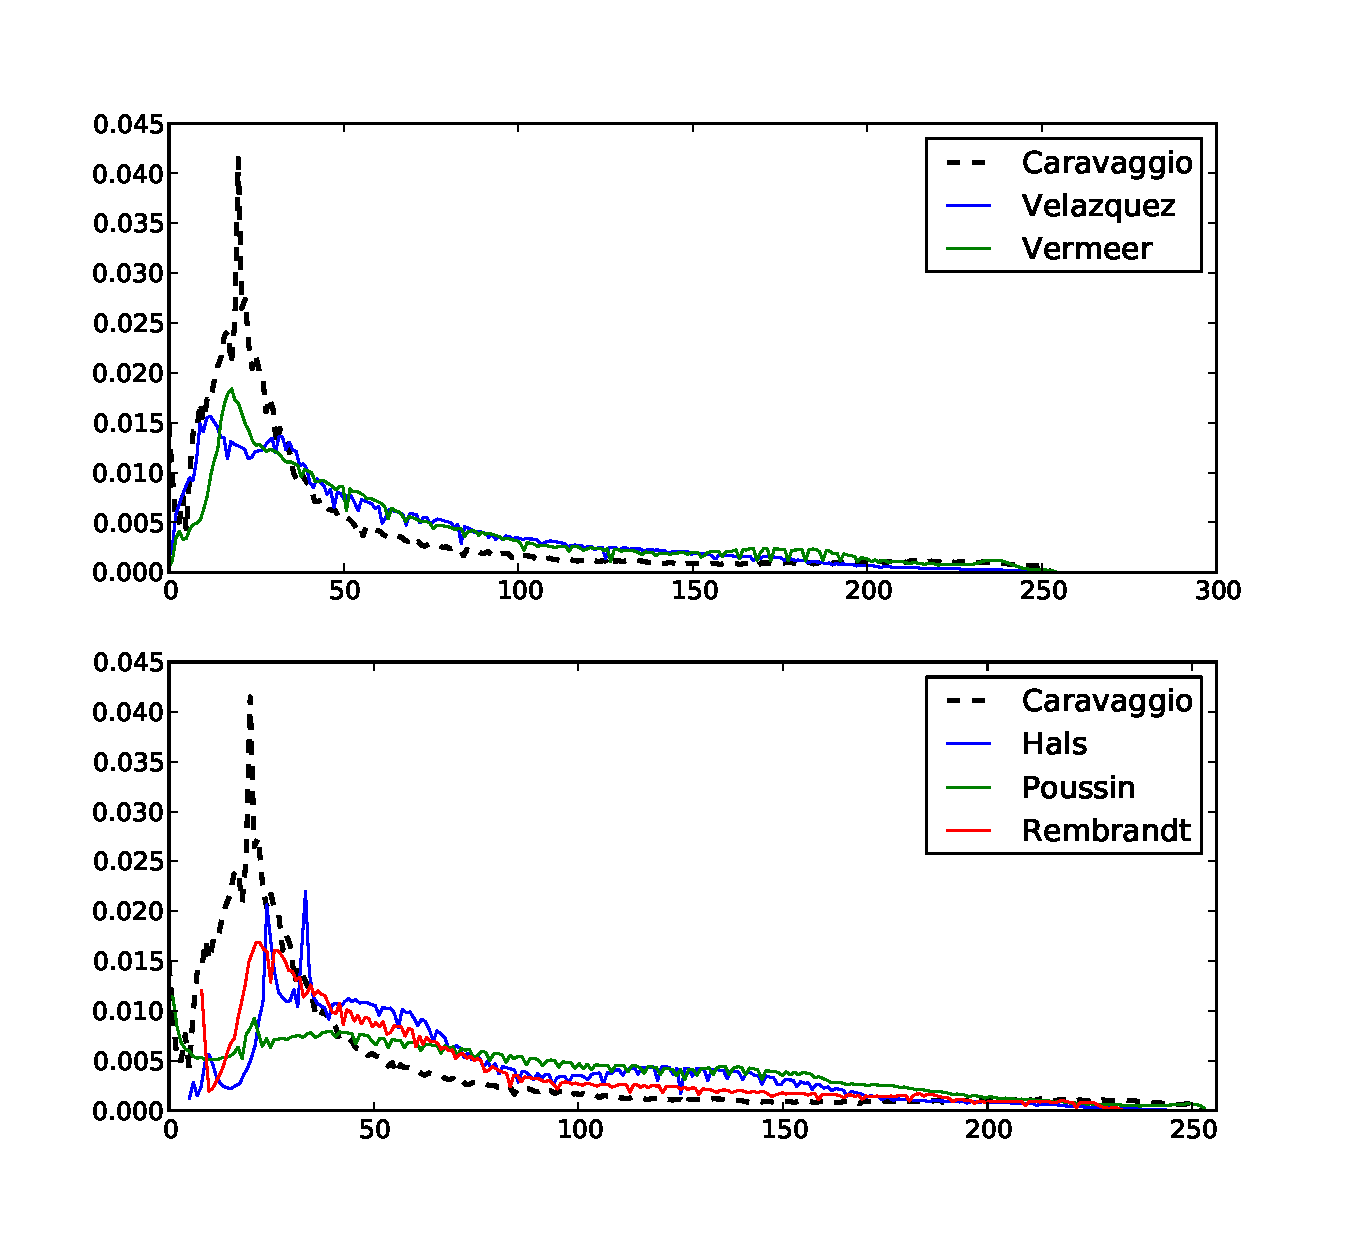
\includegraphics[width=\columnwidth]{figs/chiaroscuro}} \fonteminha \end{center}
\end{figure}

\begin{figure}[h!]
    
\begin{center}
      \caption{Histogramas nos níveis médios de cinza para os pintores
        modernos. Há baixa similaridade entre os pintores modernos, diferente do
        que ocorre para os pintores barrocos.}
        \label{fig:chiaroscuro_modernos}
{    \centering
        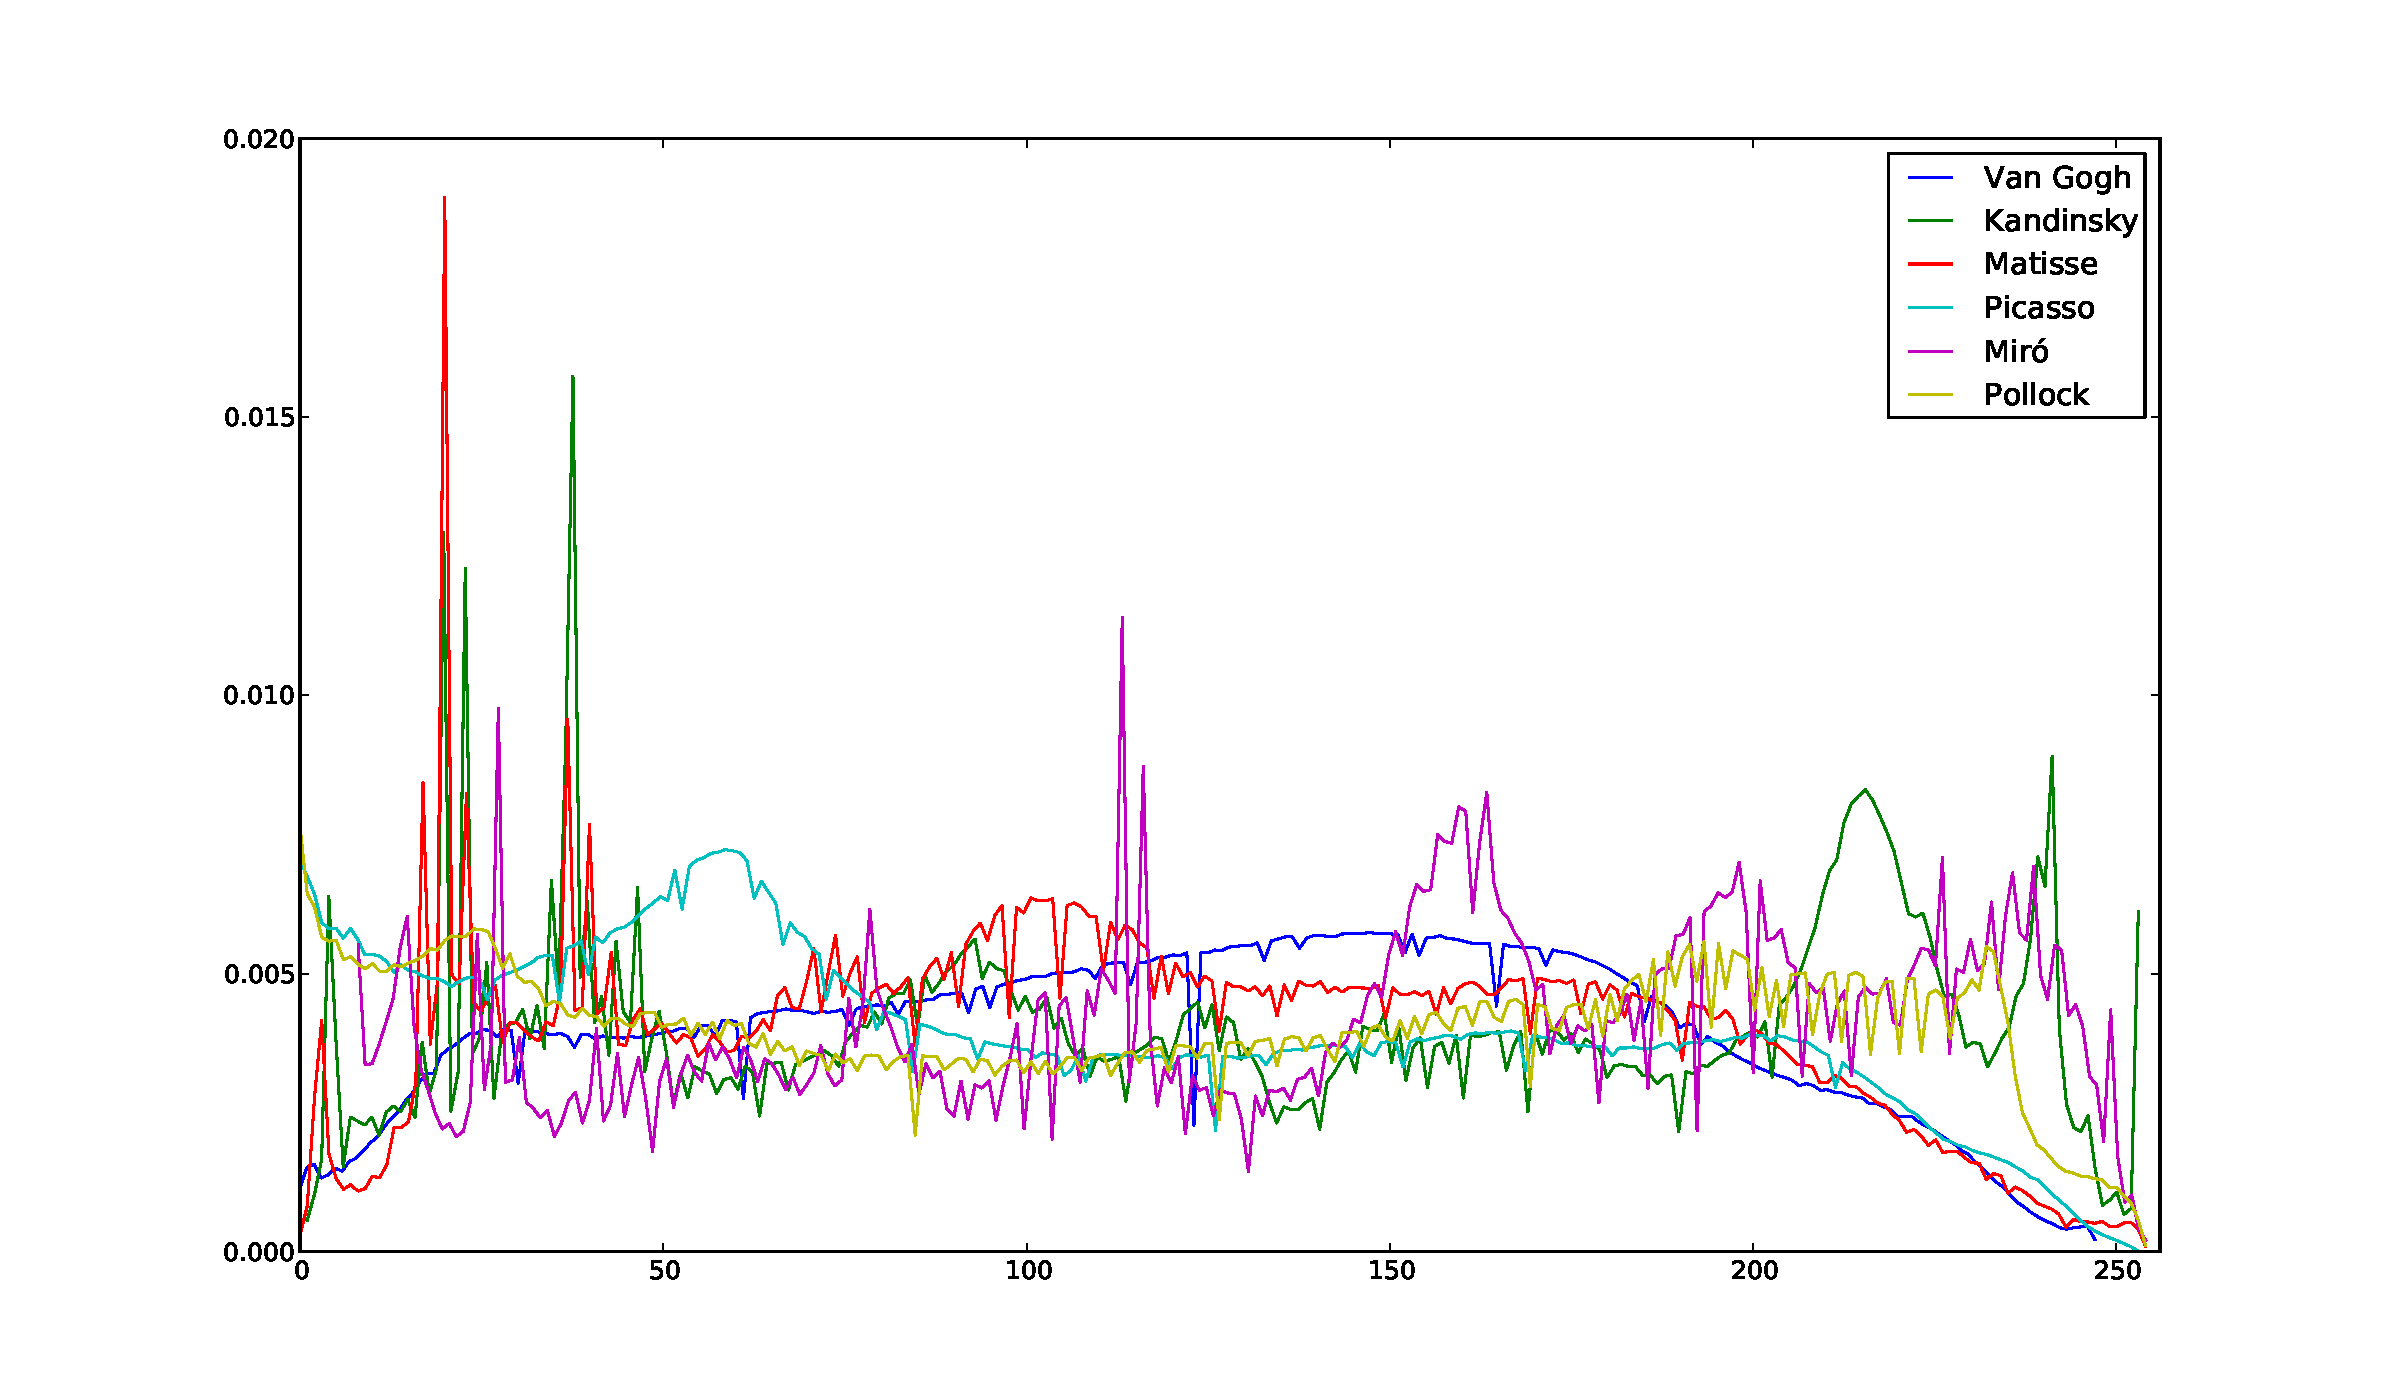
\includegraphics[width=\columnwidth]{figs/chiaroscuro_modernos}}
      \fonteminha
  \end{center}
\end{figure}

Quando são consideradas as medidas de oposição e inovação, outros
resultados interessantes apresentam-se, como mostrado na
tabela~\ref{tab:opos1} e figura~\ref{fig:caso1_oposEinov}. O maior
valor de oposição é atribuído a Rembrandt. Esse fato é curioso por si,
considerando que este pintor holandês é reconhecido como um
``contraponto'' ao movimento Barroco, mesmo tendo sido parte desse
movimento.~\cite{gombrich} Vermeer também apresenta forte oposição e a
natureza de suas pinturas (e.g.\ interiores domésticos, uso de cores
claras) pode explicar esse fenômeno. Um padrão torna-se visível no
começo de ambos períodos Barroco e Moderno: decréscimo contínuo nos
valores de oposição, seguido de acréscimo. Da mesma forma, um platô
com alta oposição é observado nos pintores barrocos. Esse platô ocorre
exatamente na transição de um período artístico ao outro, diminuindo
gradualmente enquanto os artistas modernos começam a se estabelecer na
história. Esse decréscimo dos valores de oposição reflete um aspecto
de baixa oposição entre os primeiros artistas barrocos enquanto há o
acréscimo da oposição presente nos deslocamentos que precedem o
período Moderno, embora os valores de inovação se mantém oscilando mas
aumentando durante toda a série temporal. Em resumo, no que se pode
falar dos índices de oposição e inovação, de maneira geral,
a série temporal é marcada por aumento constante de
inovação --- desconsiderando pequenas oscilações --- grande oposição em momentos específicos de sua evolução (a
transição entre o Barroco e a Arte Moderna) e menor oposição entre
artistas de um mesmo movimento, principalmente no Barroco.

% gerado com: metrics_caso1.py
\begin{table}[ht]
  \begin{center}
  \caption{\label{tab:opos1}Índice de oposição $W_{i,j}$ e inovação $s_{i,j}$
    para cada um dos 11 deslocamentos de um pintor a outro.}
\begin{tabular}{@{}lll}
    \hline \hline
    \textbf{Deslocamento} & \textbf{$W_{i,j}$} & \textbf{$s_{i,j}$} \\
    \hline
    Caravaggio $\to$ Frans Hals  &   1.     &  0.     \\
    Frans Hals $\to$ Poussin     &   0.111  &  0.425  \\
    Poussin $\to$ Velázquez   &   0.621  &  0.004  \\
    Velázquez $\to$ Rembrandt &   1.258  &  0.072  \\
    Rembrandt $\to$ Vermeer      &   1.152  &  0.341  \\
    Vermeer $\to$ Van Gogh       &   1.158  &  0.280  \\
    Van Gogh $\to$ Kandinsky     &   0.970  &  0.452  \\
    Kandinsky $\to$ Matisse      &   0.089  &  0.189  \\
    Matisse $\to$ Picasso        &   0.117  &  0.509  \\
    Picasso $\to$ Miró       &   0.385  &  0.325  \\
    Miró $\to$ Pollock       &   2.376  &  3.823  \\
    \hline \hline
  \end{tabular}
  \fonteminha
\end{center}
\end{table}

% gerado com: metrics_caso1.py
\begin{figure}[h!]
\begin{center}
         \caption{Valores de oposição $W_{i,j}$ e inovação $s_{i,j}$ considerando
        os dois melhores atributos.}
        \label{fig:caso1_oposEinov}
        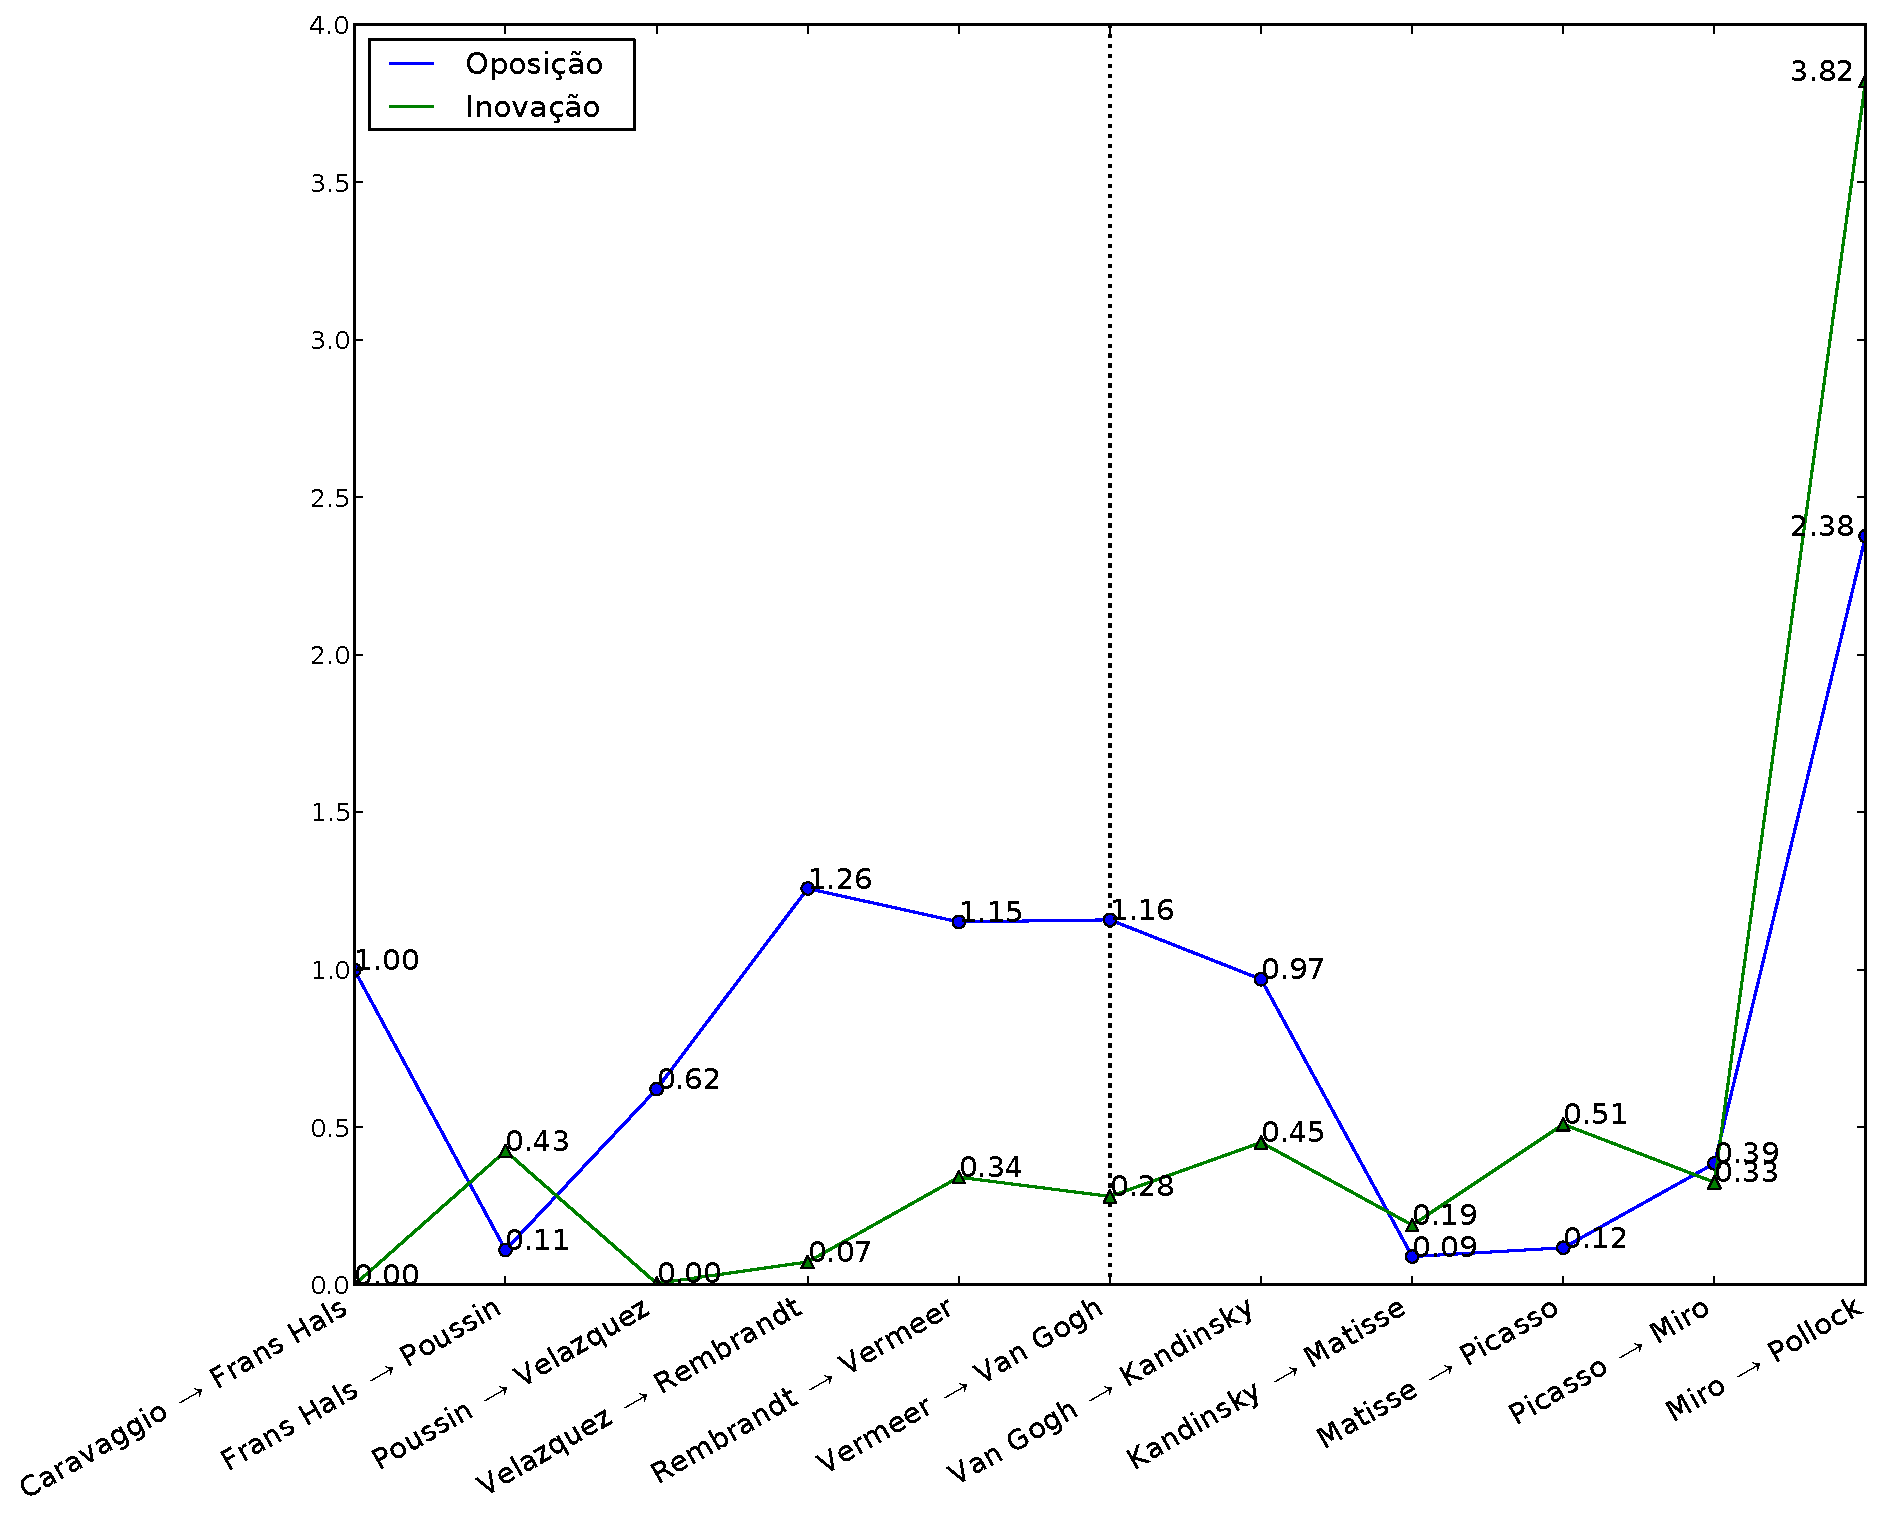
\includegraphics[width=\columnwidth]{figs/caso1_oposEinov}
        \fonteminha
\end{center}
\end{figure}

\clearpage

Além destas observações gerais sobre as medidas de oposição e
inovação, pode-se interpretar tais medidas para cada par de pintores
consecutivos. Estas observações estão apresentadas na
tabela~\ref{tab:interpretacaoOpos}.

\begin{longtable}{lllp{7cm}}
\caption{\label{tab:interpretacaoOpos} Possível interpretação, com base na história da Arte e características estéticas, para cada valor de oposição e inovação calculado. Consideram-se os dois melhores atributos: média do número de segmentos e média da quantidade de picos de curvatura.}\\

\hline \hline
\textbf{Deslocamento}       & \textbf{$W_{i,j}$} & \textbf{$s_{i,j}$} & \textbf{Possível interpretação} \\ \hline

Caravaggio $\to$ Frans Hals & 1.  & 0.  & Não é possível considerar,
pois para $i=0,j=1$ os valores de oposição e inovação serão sempre
$W_{i,j}=1$ e $s_{i,j}=0$. \\ \hline

Frans Hals $\to$ Poussin    & 0.111              & 0.425              & É a menor oposição do período Barroco e não encontra paralelo com a história, visto que Frans Hals, por ter sido influenciado por Caravaggio, deveria opor-se a Poussin. Porém, a  inovação é satisfatória, pois Poussin enfatiza a pintura de paisagens ao invés de retratos, comuns em Hals, para citar um exemplo. \\ \hline

Poussin $\to$ Velázquez     & 0.621              & 0.004              & A oposição é esperada, pois Poussin se opõe a Velázquez, que é influenciado por Caravaggio. A baixa inovação, por outro lado, não revela o esperado. \\ \hline

Velázquez $\to$ Rembrandt   & 1.258              & 0.072              & É o valor mais alto de oposição e encontra paralelo com a história: as pinturas de Rembrandt nada têm de parecido com as de Velázquez, embora se esperasse um valor maior para a inovação, dada a inventividade de Rembrandt. \\ \hline

Rembrandt $\to$ Vermeer     & 1.152              & 0.341              & Ambos valores de oposição e inovação refletem a história. Vermeer volta-se ao estilo de Caravaggio, que não possui tanta influência em Rembrandt. A inovação é a segunda mais alta do período Barroco, e corresponde ao estilo alternativo de Vermeer para a época, mesmo quando comparado a outro contraponto ao Barroco como Rembrandt. \\ \hline

Vermeer $\to$ Van Gogh      & 1.158              & 0.280              & Por se tratar de pintores de épocas muito diferentes, esperam-se valores altos para ambas oposição e inovação, talvez ainda maiores do que o apresentado. \\ \hline

Van Gogh $\to$ Kandinsky    & 0.970              & 0.452              & Espera-se alto valor de oposição dados os estilos contrastantes de ambos pintores. A inovação é alta e justifica-se, pois Kandinsky inova ao utilizar formas abstratas, não presentes nas pinturas de Van Gogh. \\ \hline

Kandinsky $\to$ Matisse     & 0.089              & 0.189              & Correspondem aos valores mais baixos de oposição e inovação do período Moderno. Embora tenham características próximas em forma, esperava-se maior oposição, dada a natureza mais abstrata de Kandinsky quando comparado a Matisse. \\ \hline

Matisse $\to$ Picasso       & 0.117              & 0.509              & A baixa oposição é esperada pois Matisse costuma retratar formas humanas assim como Picasso, com certa preferência para linhas retas ao desenhá-las. A inovação também encontra paralelo com a história, já que Picasso inaugura o Cubismo. É a maior inovação do período Moderno. \\ \hline

Picasso $\to$ Miró          & 0.385              & 0.325              & Miró se opõe e inova à Picasso com mesma intensidade. Há também fundamento na história, pois Miró é mais abstrato que Picasso, e inova no uso de pintura automática e simbólica, quase não havendo formas da realidade em suas pinturas. \\ \hline

Miró $\to$ Pollock          & 2.376              & 3.823              & Esse alto contraste é esperado. Pollock é o pintor que mais se diferencia de todos os demais pintores, inclusive Miró. \\ \hline \hline

\fonteminha
\end{longtable}

No que tange a contra-dialética, mostrada na
tabela~\ref{tab:dialetica1} e figura~\ref{fig:caso1_dialetica}, há um
paralelo com a curva de oposição. A contra-dialética reforça fatos já
observados: pintores do mesmo período apresentam inicialmente
decréscimo em seus valores, seguido por acréscimo contínuo. O pico de
contra-dialética acontece em Van Gogh e Kandinsky: exatamente o ponto
onde o Barroco termina e a Arte Moderna começa. A
tabela~\ref{tab:interpretacaoDia} oferece uma possível interpretação
para cada valor de dialética calculado, ao compará-los com a história
da Arte.

% gerado com: metrics_caso1.py
\begin{table}[ht]
  \begin{center}
  \caption{\label{tab:dialetica1} Índices de contra-dialética para cada um dos
    10 deslocamentos entre tese, antítese e síntese, considerando os dois
    melhores atributos: média do número de segmentos e média da quantidade de picos de curvatura.}
\begin{tabular}{@{}ll}
  
    \hline \hline
    \textbf{Tese, antítese e síntese} & \textbf{$d_{i \rightarrow k}$} \\
    \hline
    Caravaggio $\to$ Frans Hals $\to$ Poussin   & 0.572 \\
    Frans Hals $\to$ Poussin $\to$ Velázquez & 0.337 \\
    Poussin $\to$ Velázquez $\to$ Rembrandt  & 0.151 \\
    Velázquez $\to$ Rembrandt $\to$ Vermeer  & 0.608 \\
    Rembrandt $\to$ Vermeer $\to$ Van Gogh      & 1.362 \\
    Vermeer $\to$ Van Gogh $\to$ Kandinsky      & 1.502 \\
    Van Gogh $\to$ Kandinsky $\to$ Matisse      & 1.062 \\
    Kandinsky $\to$ Matisse $\to$ Picasso       & 0.183 \\
    Matisse $\to$ Picasso $\to$ Miró         & 0.447 \\
    Picasso $\to$ Miró $\to$ Pollock         & 2.616 \\
    \hline \hline
  \end{tabular}
  \fonteminha
\end{center}
\end{table}


% gerado com: metrics_caso1.py
\begin{figure}[h!]
\begin{center}
       \caption{Valores de contra-dialética considerando os dois melhores atributos.}
        \label{fig:caso1_dialetica}
        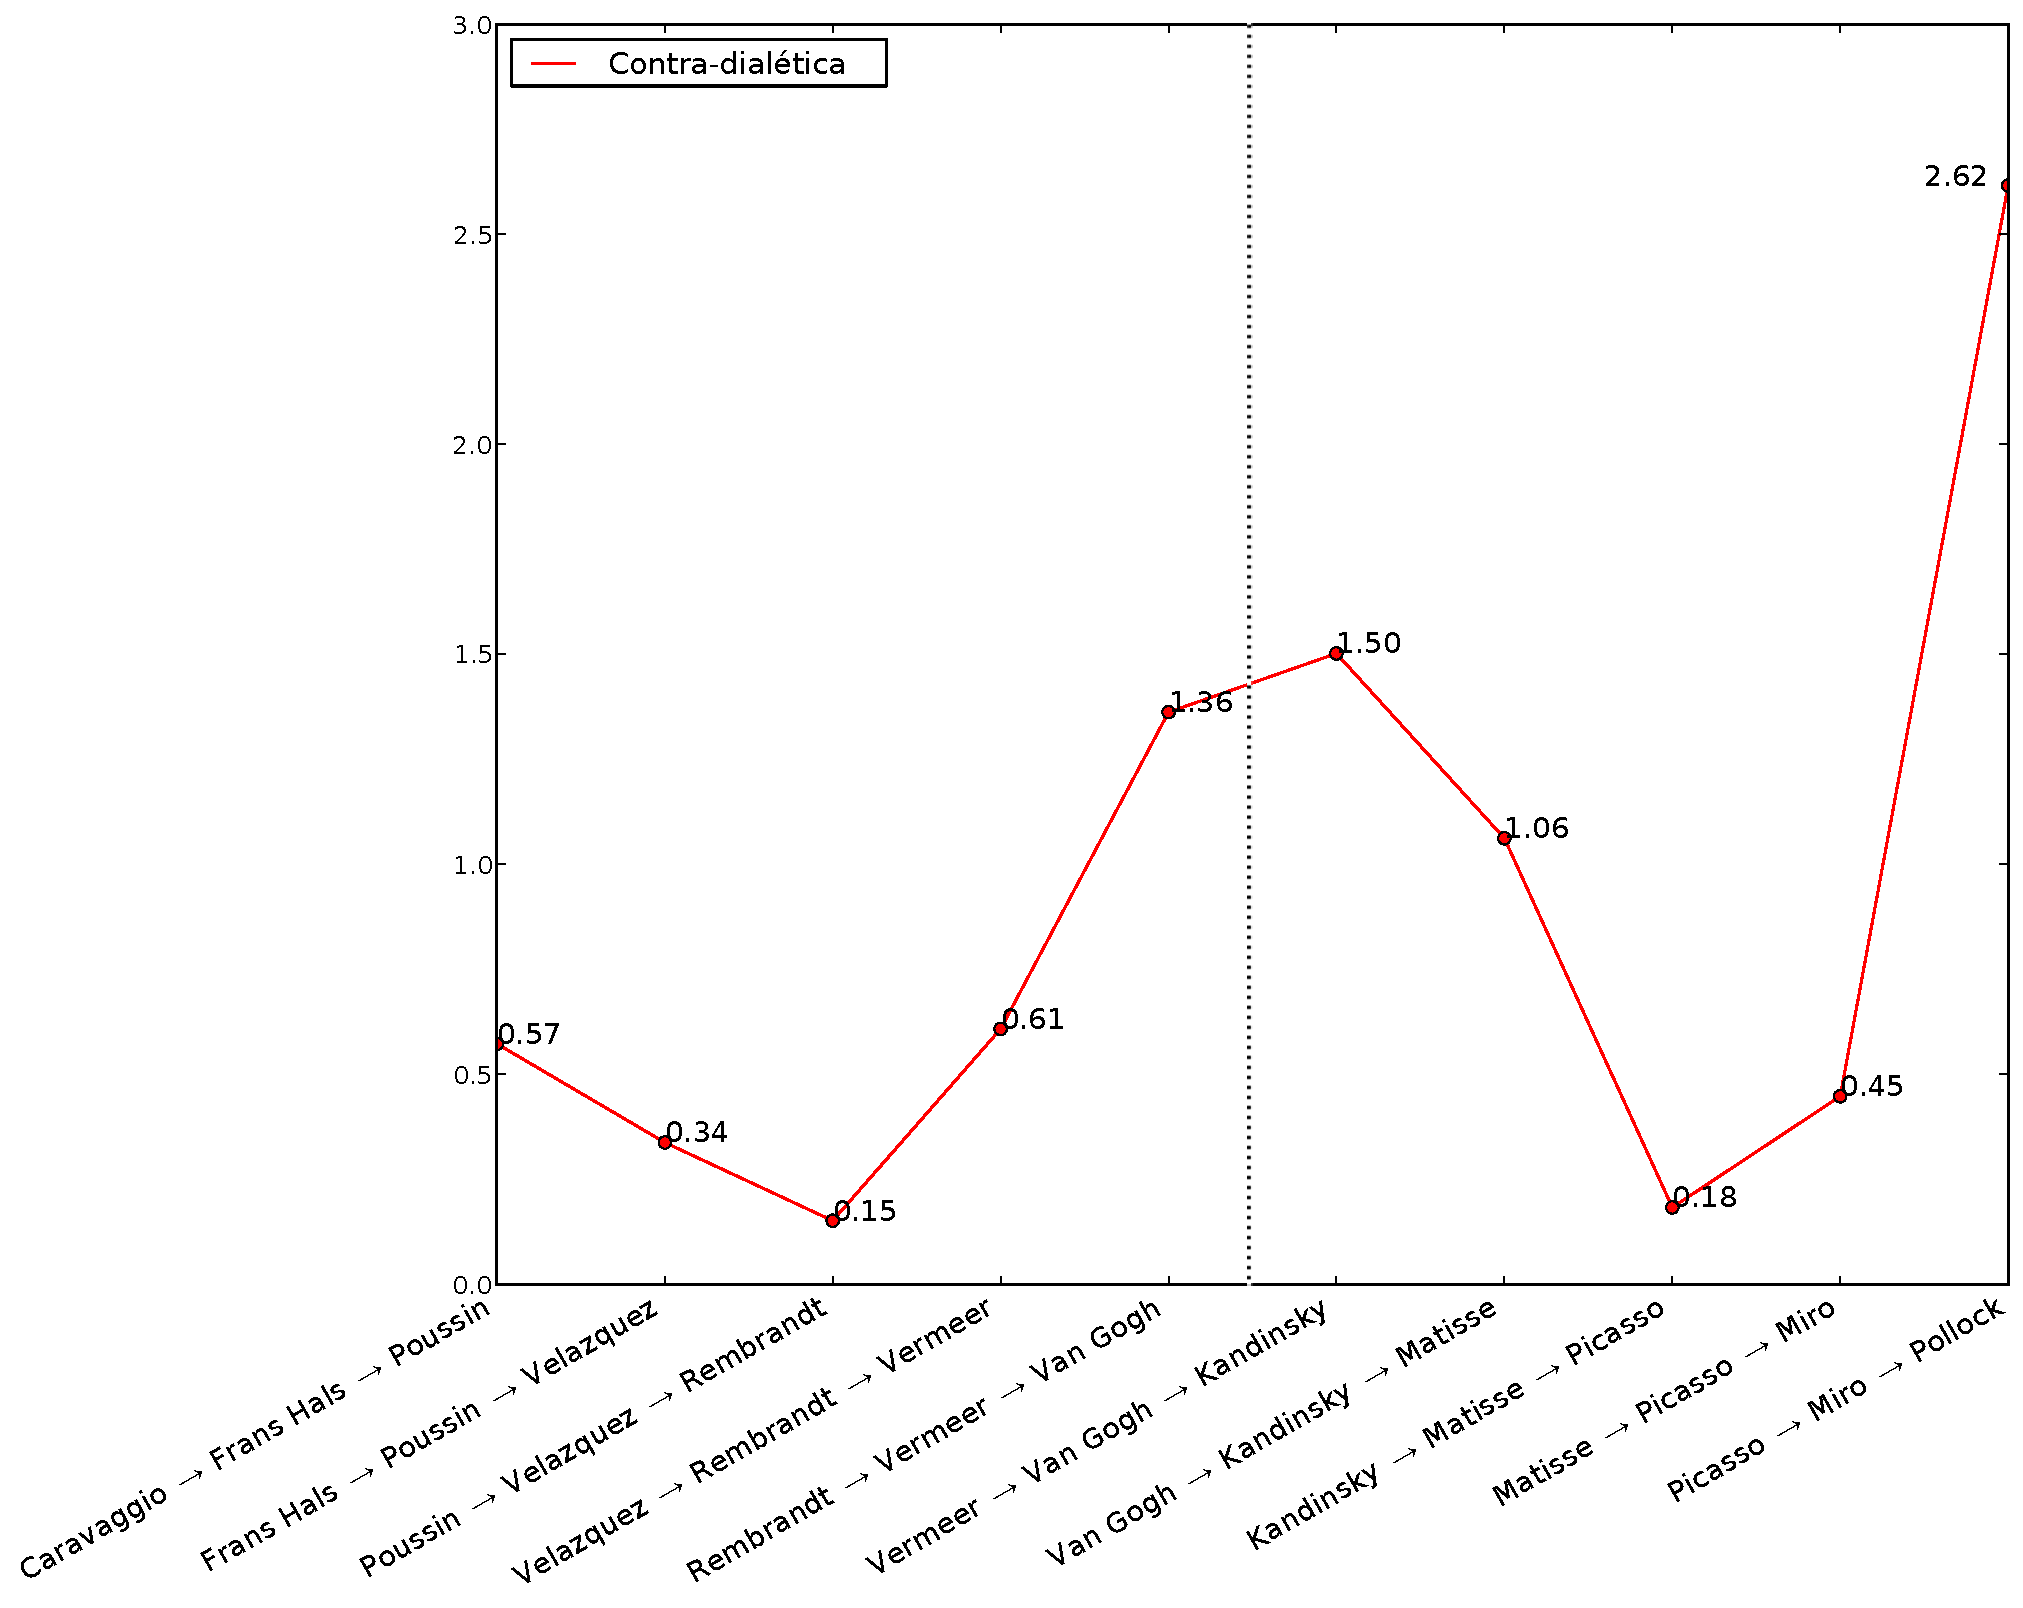
\includegraphics[width=\columnwidth]{figs/caso1_dialetica}
        \fonteminha
\end{center}
\end{figure}




\begin{longtable}{llp{8cm}}
\caption{\label{tab:interpretacaoDia} Possível interpretação, com base na história da Arte e características estéticas, para cada valor de contra-dialética calculado.}\\

\hline \hline
\textbf{Tese, antítese e síntese}       & \textbf{$d_{i \rightarrow k}$} & \textbf{Possível interpretação} \\ \hline

Caravaggio $\to$ Frans Hals $\to$ Poussin   & 0.572 &
Poussin, segundo a história da Arte, não representa a síntese entre
Caravaggio e Frans Hals. Pelo contrário, Poussin distancia-se de ambos pintores.
Portanto, o valor de contra-dialética corresponde ao esperado. \\ \hline

Frans Hals $\to$ Poussin $\to$ Velázquez & 0.337 &
Espera-se também que Velázquez afaste-se da síntese entre Frans Hals e Poussin,
já que Velázquez assemelha-se mais a Frans Hals. \\ \hline

Poussin $\to$ Velázquez $\to$ Rembrandt  & 0.151 &
É a maior dialética de toda a série, e encontra fundamento na história. Rembrandt,
dada sua inventividade, parece ter explorado tanto paisagens (como Poussin) quanto
retratos utilizando \textit{chiaroscuro} (como Velázquez). \\ \hline

Velázquez $\to$ Rembrandt $\to$ Vermeer  & 0.608 &
Vermeer realmente difere de ambos Velázquez e Rembrandt, pintando em um estilo
alternativo para a época, portanto o valor alto de contra-dialética é
justificado. \\ \hline

Rembrandt $\to$ Vermeer $\to$ Van Gogh      & 1.362 &
Sendo um pintor moderno, Van Gogh se opõe aos pintores Barrocos e este aumento abrupto
de contra-dialética é esperado, pois é neste instante que se dá a transição de
um período para o outro. \\ \hline

Vermeer $\to$ Van Gogh $\to$ Kandinsky      & 1.502 &
Kandinsky, um pintor abstrato, apresenta a maior contra-dialética da série
(desconsiderando-se Pollock). Realmente não possui semelhanças com ambos Vermeer e Van Gogh. \\ \hline

Van Gogh $\to$ Kandinsky $\to$ Matisse      & 1.062 &
Matisse distancia-se da síntese entre Van Gogh e Kandinsky. Embora suas pinturas
tenham formas humanas e com variações de cores, como as de Van Gogh, não são abstratas como as de Kandinsky. \\ \hline

Kandinsky $\to$ Matisse $\to$ Picasso       & 0.183 &
Picasso realmente parece combinar elementos abstratos (e.g. figuras geométricas presentes em Kandinsky) com formas encontradas na natureza e figuras humanas, pintadas também por Matisse. Espera-se portanto alta dialética. \\ \hline

Matisse $\to$ Picasso $\to$ Miró         & 0.447 &
Por ser um pintor abstrato, espera-se que Miró se distancie da síntese entre Matisse e Picasso, principalmente por Matisse não empregar formas abstratas. Porém, isto não é
revelado pelo valor de contra-dialética. \\ \hline

Picasso $\to$ Miró $\to$ Pollock         & 2.616 &
Assim como para as medidas de oposição e inovação, Pollock apresenta o maior valor de
contra-dialética da série, dada a natureza de suas obras, que diferem de todos os
demais pintores considerados.
\\ \hline \hline

\fonteminha
\end{longtable}


\clearpage
\section{Análise por LDA de todos os atributos}
\label{subsec:lda}

Embora os atributos \emph{média de picos de curvatura} e \emph{média
  do número de segmentos} apresentaram-se como opções interessantes
para a classificação, o método LDA foi aplicado considerando todos os
$N = 100$ atributos com o objetivo de testar a relevância dos atributos
originalmente selecionados e a estabilidade dos resultados. O método
LDA projeta os atributos em um espaço de $r < N$ dimensões que melhor
separa as pinturas e que acaba por resultar em uma nova série temporal
como feito para o caso dos melhores atributos. Nesse caso, para
permitir a visualização das medidas, considerou-se a projeção com $r =
2$ componentes que resultou em um espaço de 2 dimensões, mostrado na
figura~\ref{fig:caso3_g1}. É possível notar que os resultados para a
análise por LDA são ainda mais aparentes do que aqueles obtidos na
seção~\ref{sec:pares}: os índices de inovação
(tabela~\ref{tab:opos3} e figura~\ref{fig:caso3_oposEinov}) apresentam uma curva ascendente
ainda mais bem definida durante toda a evolução da série. Os padrões
notados na evolução de ambos índices de oposição e contra-dialética
continuam visíveis nessa nova projeção por LDA, como é possível notar
na figura~\ref{fig:caso3_oposEinov}, tabela~\ref{tab:dialetica3} e figura~\ref{fig:caso3_dialetica}.

% gerado com: metrics_caso3.py
\begin{figure}[h!]
\begin{center}
        \caption{Série temporal resultante da projeção em 2 dimensões do
        \textit{espaço criativo} considerando os dois primeiros componentes com
        maiores autovalores obtidos a partir da transformação LDA na matriz de
        $N = 100$ atributos.}
        \label{fig:caso3_g1}
        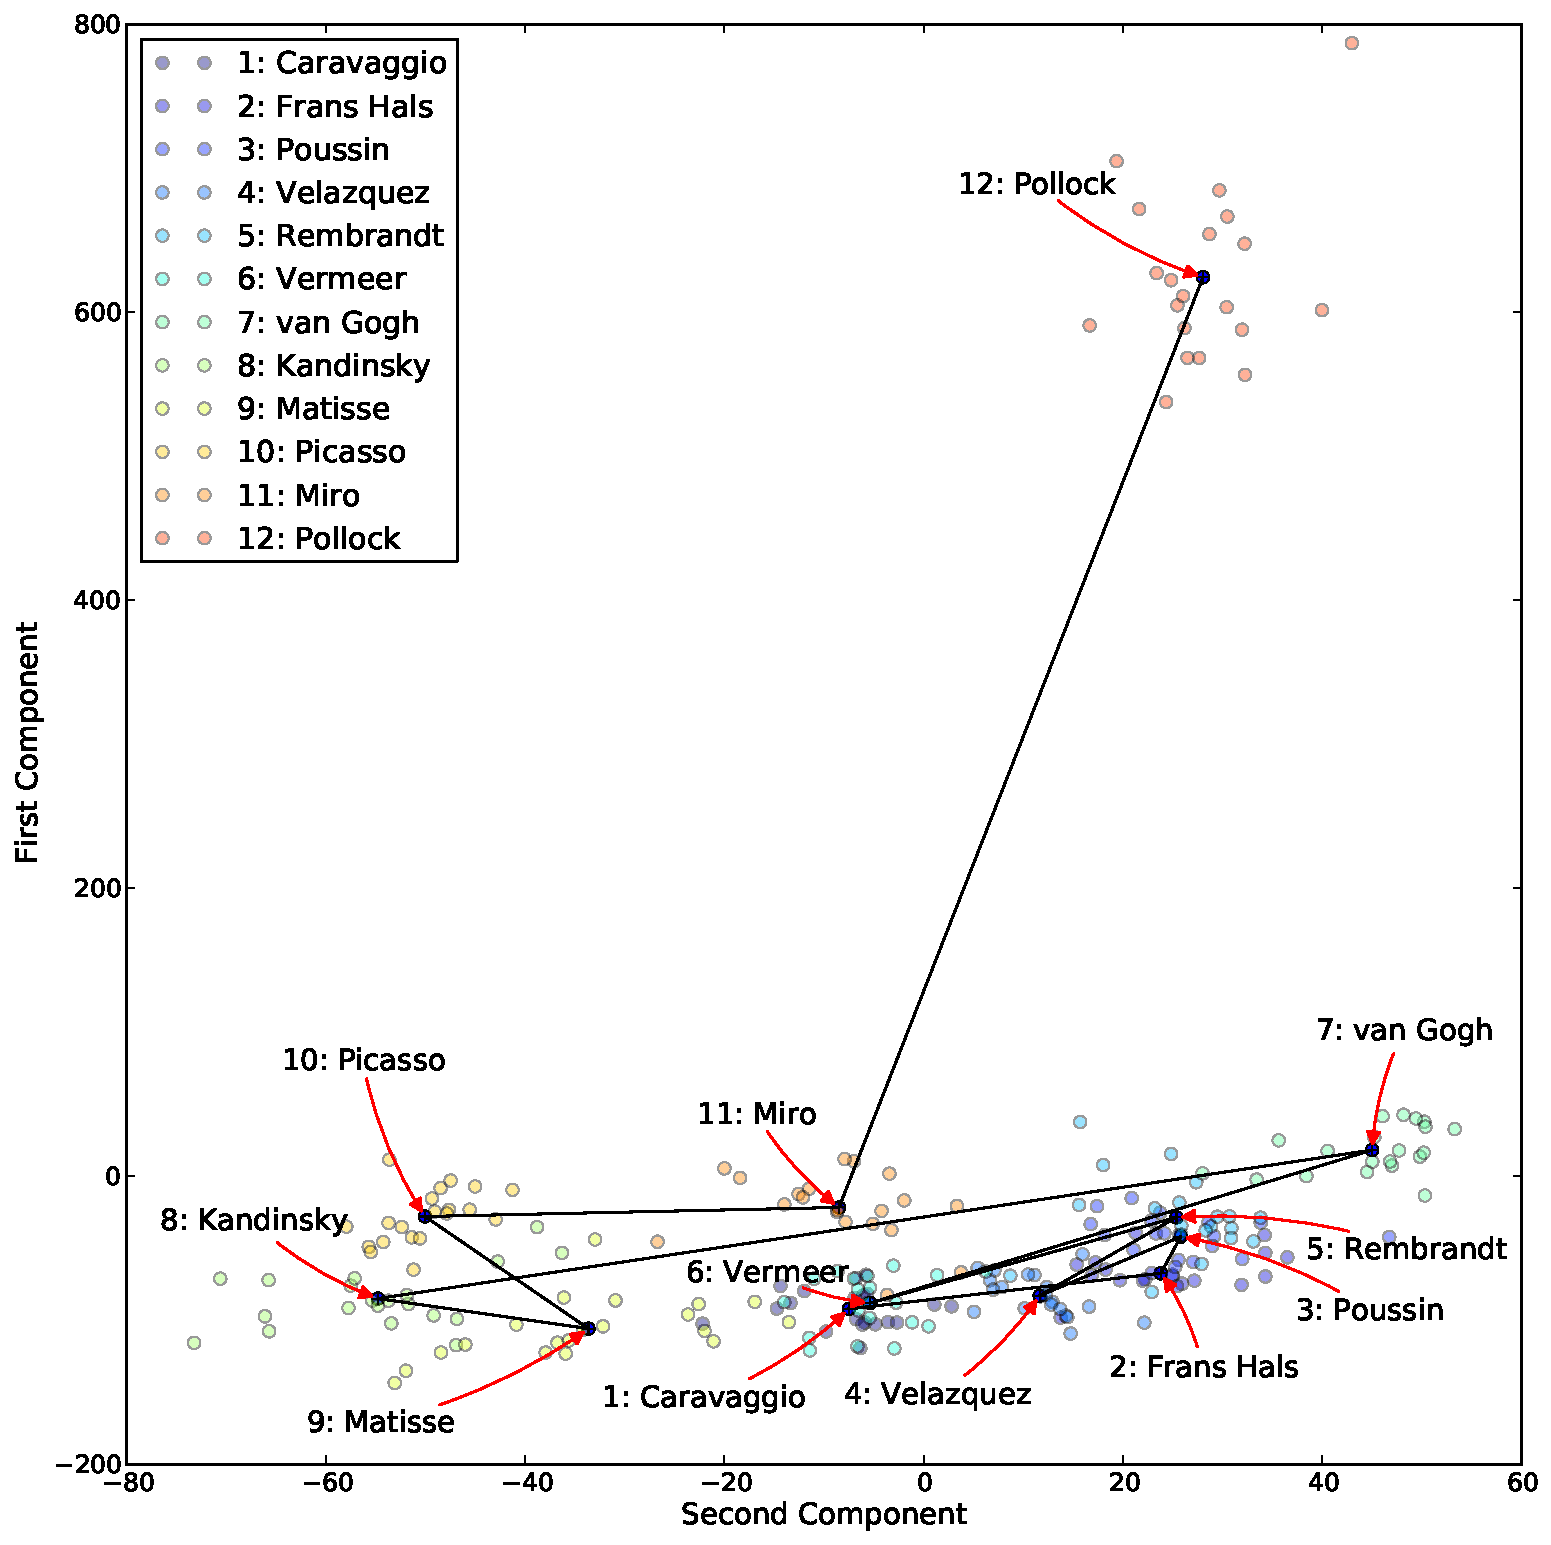
\includegraphics[width=\columnwidth]{figs/caso3_g1}
        \fonteminha
\end{center}
\end{figure}

% gerado com: metrics_caso3.py
\begin{table}[ht]
  \begin{center}
\caption{\label{tab:opos3}Índices de oposição e inovação para cada um dos 11
  deslocamentos de um pintor ao outro.}
\begin{tabular}{@{}lll}
    \hline \hline
    \textbf{Deslocamento} & \textbf{$W_{i,j}$} & \textbf{$s_{i,j}$} \\
    \hline
    Caravaggio $\to$ Frans Hals  &   1.     &  0.     \\
    Frans Hals $\to$ Poussin     &  -0.101  &  0.132  \\
    Poussin $\to$ Velázquez   &   0.588  &  0.037  \\
    Velázquez $\to$ Rembrandt &   1.526  &  0.050  \\
    Rembrandt $\to$ Vermeer      &   1.101  &  0.143  \\
    Vermeer $\to$ Van Gogh       &   1.153  &  0.157  \\
    Van Gogh $\to$ Kandinsky     &   1.279  &  0.512  \\
    Kandinsky $\to$ Matisse      &   0.179  &  0.149  \\
    Matisse $\to$ Picasso        &  -0.201  &  0.516  \\
    Picasso $\to$ Miró       &   0.432  &  0.163  \\
    Miró $\to$ Pollock       &   4.031  &  2.662  \\
    \hline \hline
  \end{tabular}
  \fonteminha
\end{center}
\end{table}

% gerado com: metrics_caso3.py
\begin{figure}[h!]
\begin{center}
      \caption{Valores de oposição e inovação considerando a série temporal para
        todos os $N = 100$ atributos refletidos nos dois primeiros componentes
        obtidos pelo método LDA. Os mesmos padrões observados quando
        considerando os dois melhores atributos ainda permanecem nessa
        observação, como esperado.}
        \label{fig:caso3_oposEinov}
        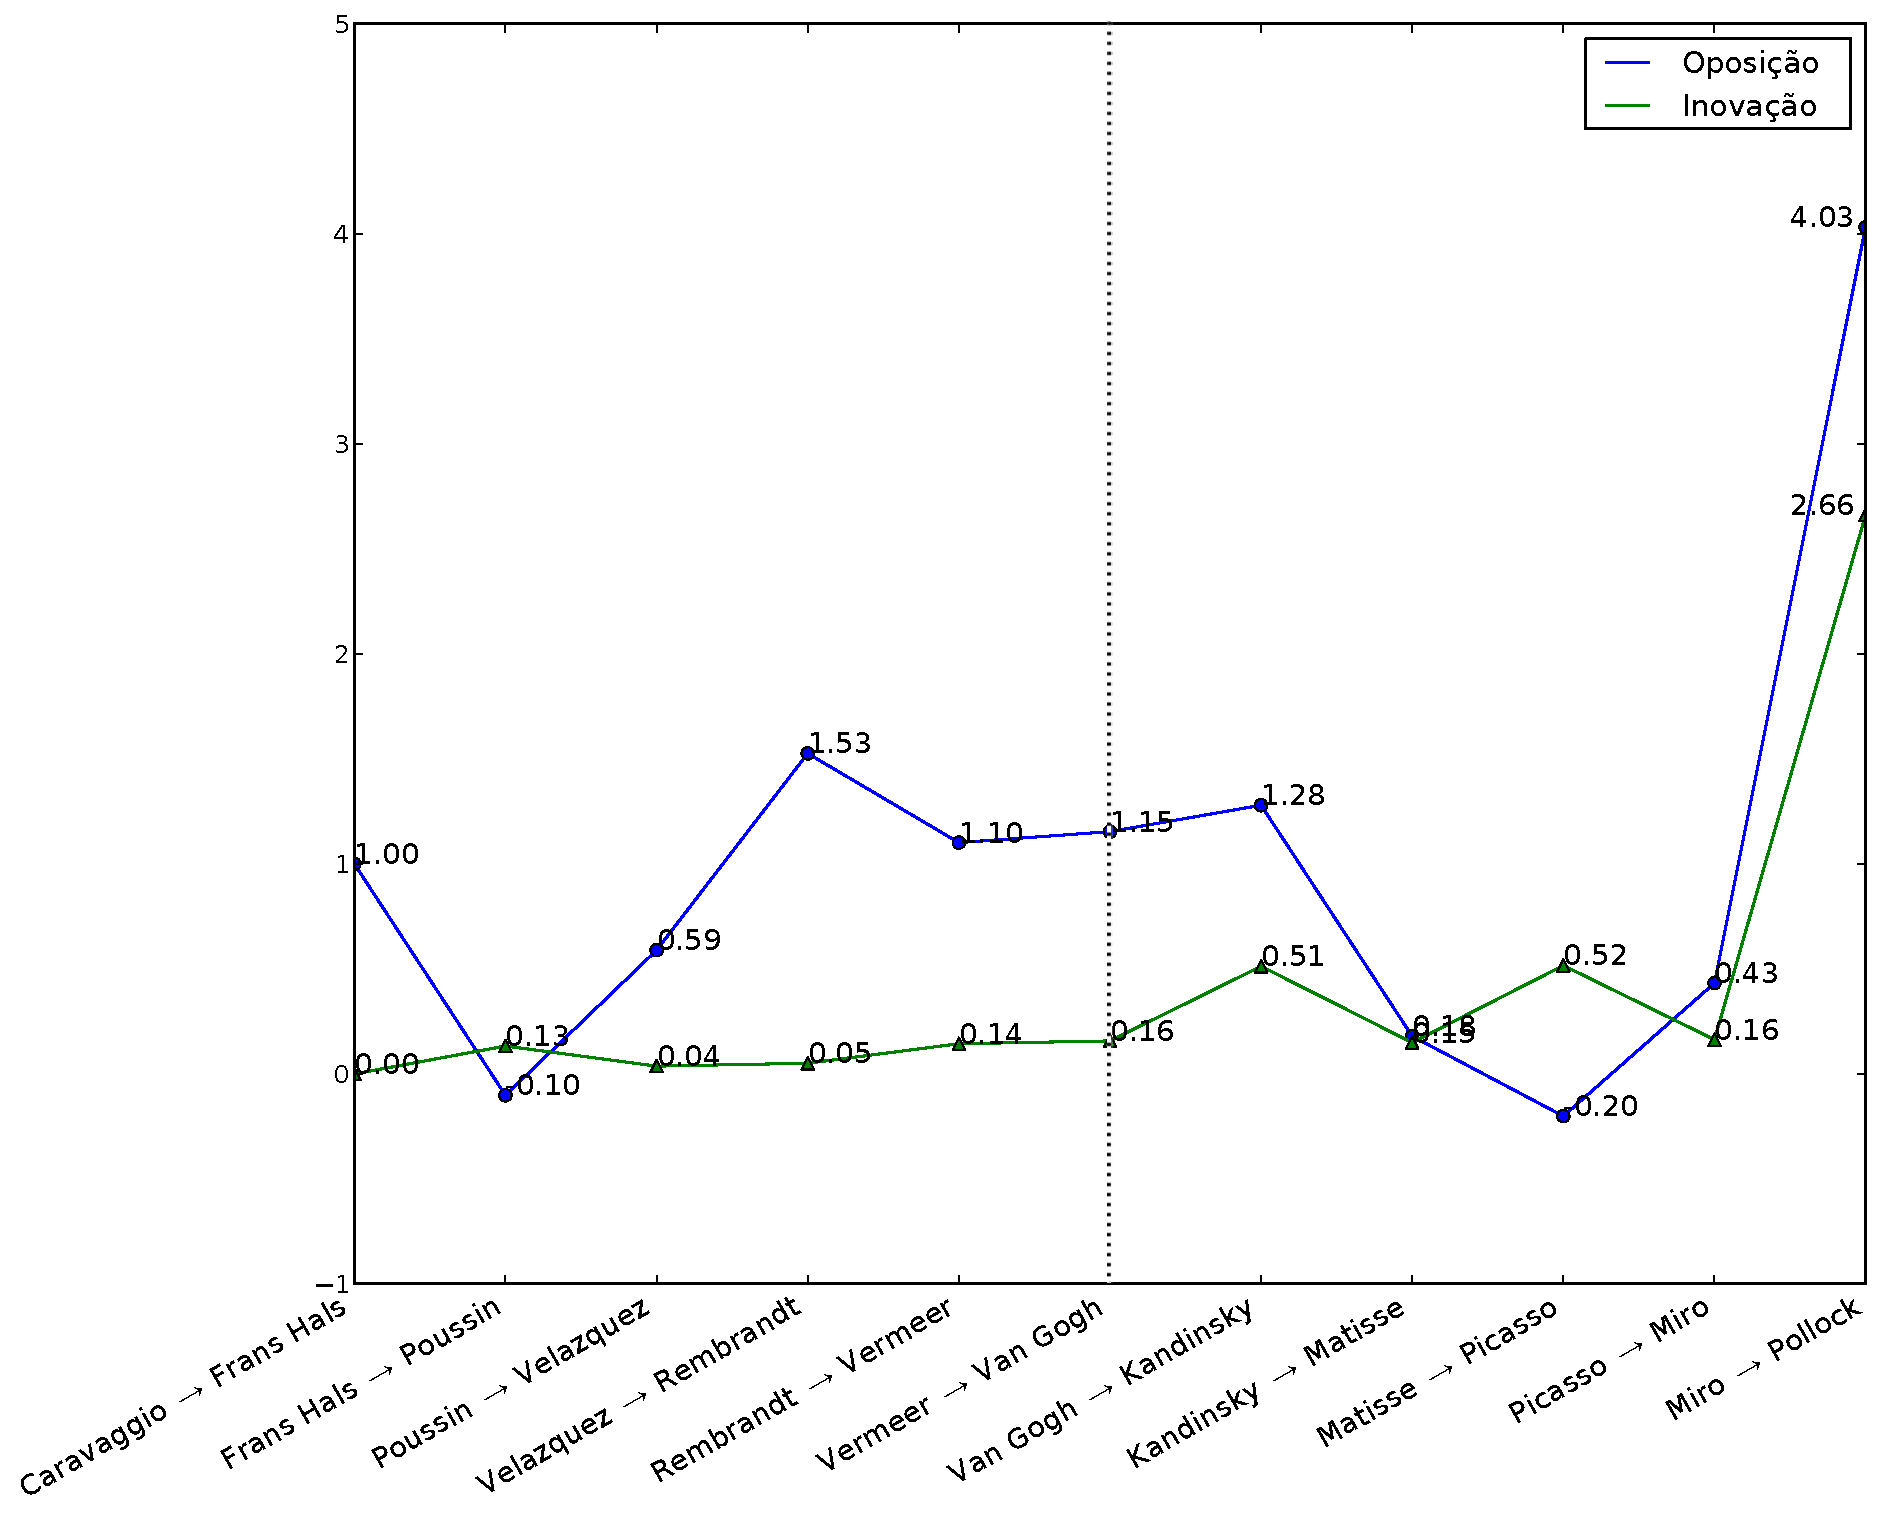
\includegraphics[width=\columnwidth]{figs/caso3_oposEinov}
       \fonteminha
\end{center}
\end{figure}

% gerado com: metrics_caso1.py
\begin{table}[ht]
  \begin{center}
  \caption{\label{tab:dialetica3} Índices de contra-dialética para cada um dos
    deslocamentos para os dois melhores componentes do LDA.}
\begin{tabular}{@{}ll}
    \hline \hline
    \textbf{Deslocamento} & \textbf{Contra-dialética ($d_{i \rightarrow k}$)} \\
    \hline
    Caravaggio $\to$ Frans Hals $\to$ Poussin   & 0.587 \\
    Frans Hals $\to$ Poussin $\to$ Velázquez & 0.317 \\
    Poussin $\to$ Velázquez $\to$ Rembrandt  & 0.268 \\
    Velázquez $\to$ Rembrandt $\to$ Vermeer  & 0.736 \\
    Rembrandt $\to$ Vermeer $\to$ Van Gogh      & 1.192 \\
    Vermeer $\to$ Van Gogh $\to$ Kandinsky      & 2.352 \\
    Van Gogh $\to$ Kandinsky $\to$ Matisse      & 0.974 \\
    Kandinsky $\to$ Matisse $\to$ Picasso       & 0.241 \\
    Matisse $\to$ Picasso $\to$ Miró         & 0.704 \\
    Picasso $\to$ Miró $\to$ Pollock         & 1.924 \\
    \hline \hline
  \end{tabular}
  \fonteminha
  \end{center}
\end{table}


% gerado com: metrics_caso3.py
\begin{figure}[h!]
\begin{center}
      \caption{Contra-dialética (valores altos indicam baixa
        incidência de dia\-lé\-ti\-ca) calculada para os componentes principais
        obtidos por LDA. O padrão observado anteriormente para o melhor par de
        atributos apresenta-se ainda mais visível aqui: é possível observar
        claramente que o maior valor está no ponto de transição dos movimentos
        artísticos (Van Gogh e Kandinsky).}
        \label{fig:caso3_dialetica}
        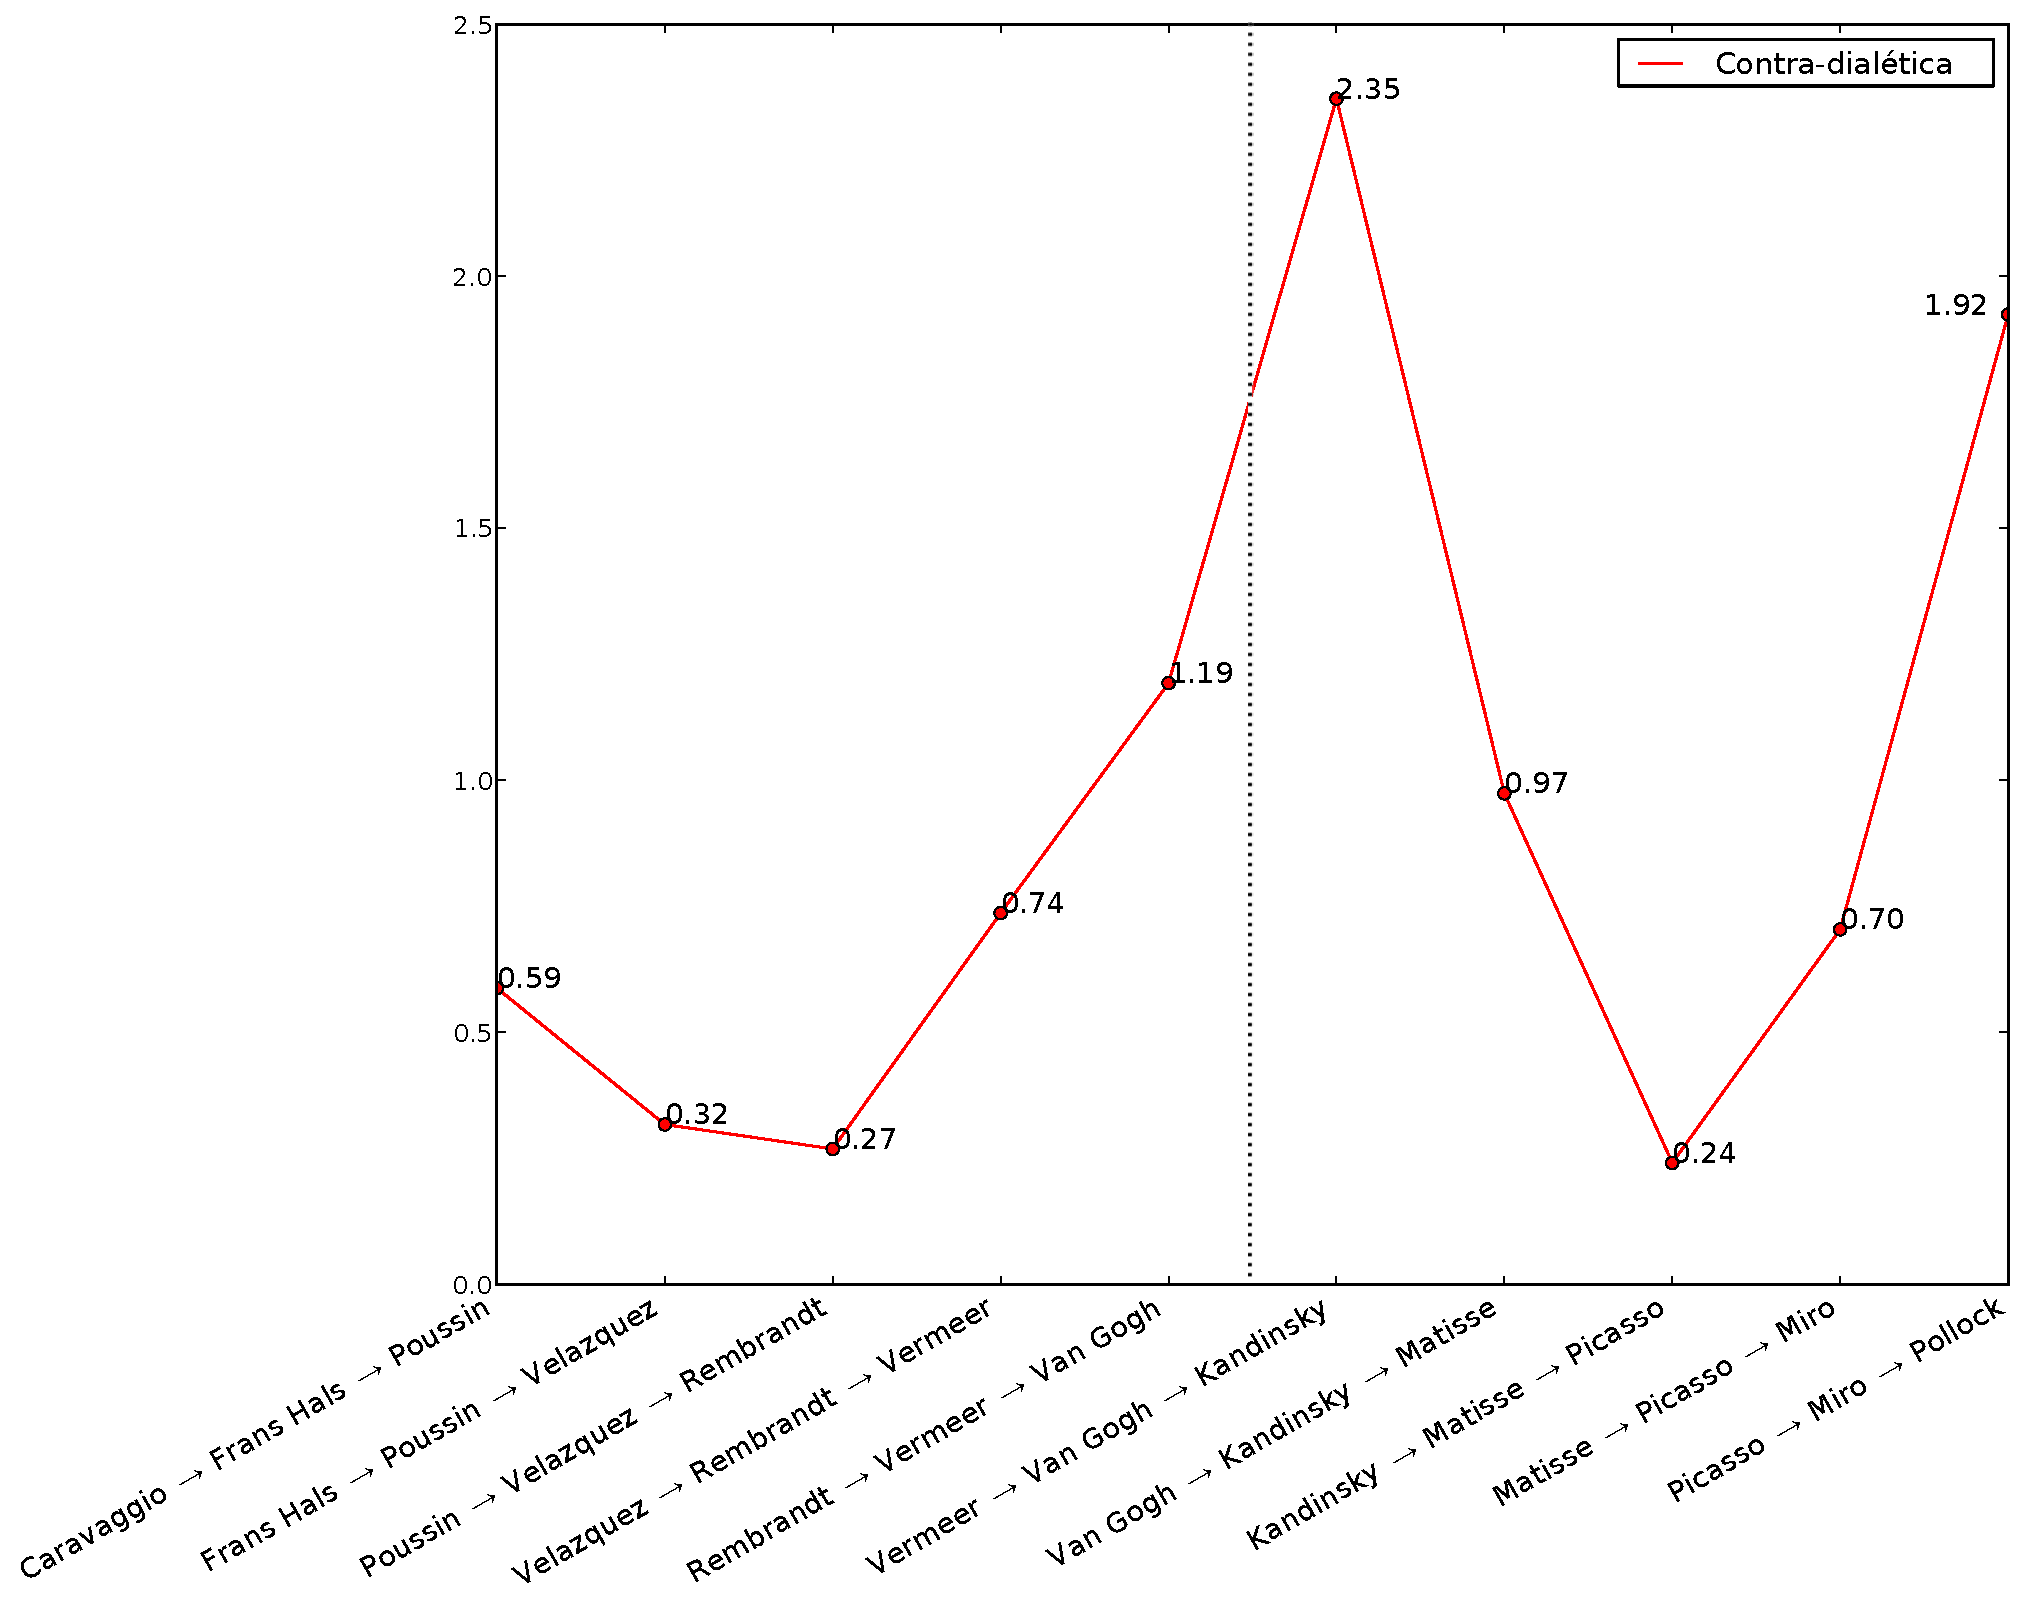
\includegraphics[width=\columnwidth]{figs/caso3_dialetica}
        \fonteminha
\end{center}
\end{figure}

Para validação do LDA aplicou-se \textit{cross validation}
por \textit{repeated random sub-sampling}. O grupo de 240 pinturas foi
dividido em dois: um conjunto de treinamento contendo 10 pinturas
selecionadas aleatoriamente para cada artista, e um conjunto de teste
contendo as 10 pinturas restantes para cada artista, ambos sem
repetição. A matriz de confusão indica o quão satisfatória é a
classificação. O cálculo da matriz de confusão foi repetido 100 vezes
e a figura~\ref{fig:cm} mostra a matriz de confusão média. Ainda, a
função de acurácia foi calculada em cada uma das repetições e teve seu
valor em média ultrapassando $58\%$ de acurácia. Os elementos da
diagonal principal representam o número de amostras (pinturas) para as
quais a classe obtida no conjunto de teste coincide com a classe
esperada (obtida na fase de treinamento). Elementos localizados fora
da diagonal principal indicam aquelas amostras que não foram
classificadas corretamente. Quanto maiores os valores
da diagonal principal, melhor a predição de classes. Como é possível
observar, o método LDA demonstra predição esperada para o grupo de
pinturas considerado. As amostras com melhor classificação são as
pinturas de Pollock, o que é esperado, pois é o pintor que mais se
distancia dos outros no \textit{espaço criativo}. Em geral, a matriz
de confusão reflete os resultados previamente discutidos: há
similaridade entre pintores barrocos, principalmente Velázquez,
Caravaggio e Rembrandt e é possível notar claramente a separação entre
pintores anteriores e posteriores a Van Gogh, que define a fronteira
entre os períodos Barroco e Moderno. Porém, o desempenho do método LDA para Miró e Rembrandt não corresponde ao esperado, sendo estes
os piores resultados da matriz de confusão.

%% gerado com: ga-delaunay/matriz_confusao.py
\begin{figure}[h!]
\begin{center}
      \caption{Matriz de confusão média para o método LDA calculada
        durante 100 iterações. Metade das pinturas de cada artista é
        usada como conjunto de treino e a metade restante como
        conjunto de teste. Os elementos da diagonal principal mostram
        o número de amostras da classe esperada que correspondem com a
        classe obtida pelo método. Dada a grande quantidade de valores
        na diagonal principal, a validação sugere que o método LDA foi
        suficiente para a classificação das pinturas. Além disso,
        detalhes já observados nos resultados desse estudo são
        novamente observados na matriz: separação entre os pintores
        antecessores e sucessores à Van Gogh e similaridade entre
        pintores do mesmo período, principalmente Barroco. A função de
        acurácia também foi calculada, equivalendo em média a $58\%$
        para as repetições
        consideradas.}  \label{fig:cm} 
     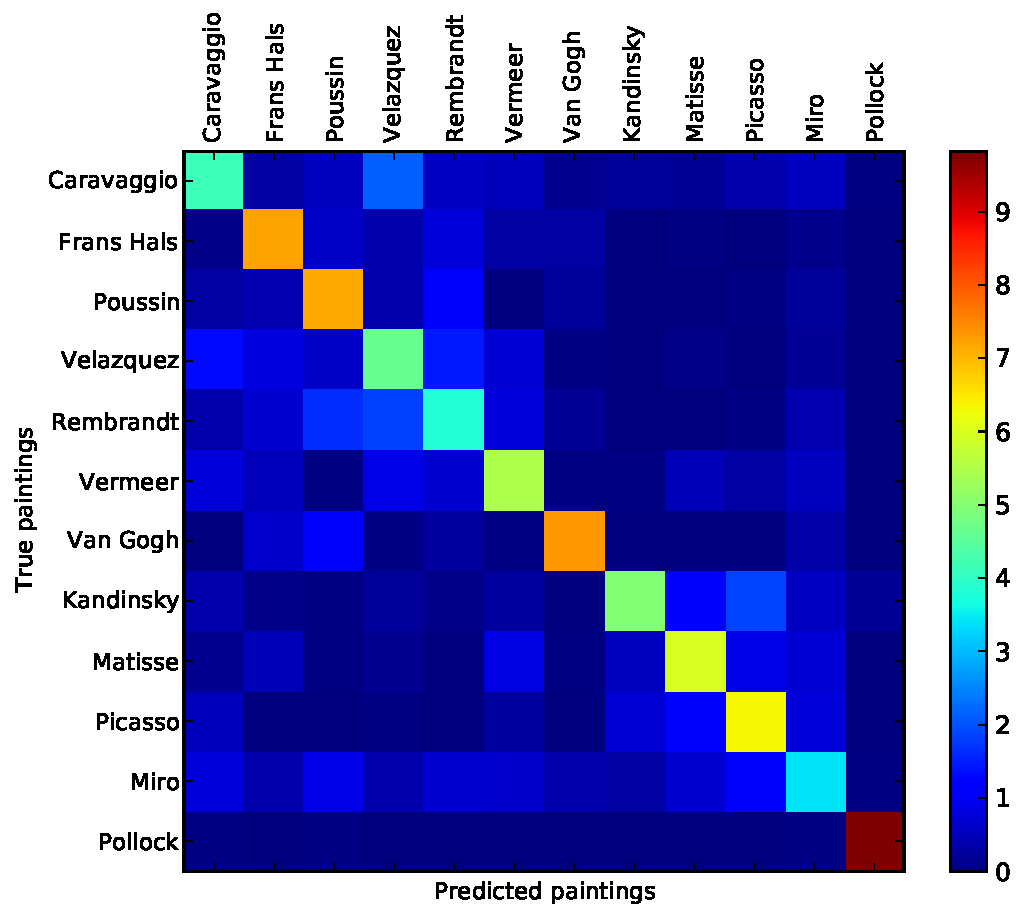
\includegraphics[width=\columnwidth]{figs/matriz_confusao} \fonteminha
\end{center}
\end{figure}

%%%%%%%%%%%%%%%%%%%%%%%%%%%%%%%%%%%%%%%%%%%%%%%%%%%%%%%%%%%%%%%%%%%%%%%%%%%
%%%%%%%%%%%%%%%%%%%%%%%%%%%%%%%%%%%%%%%%%%%%%%%%%%%%%%%%%%%%%%%%%%%%%%%%

%%%%%%%%%%%%%%%%%%%%%%%%%%%%%%%%%%%%%%%%%%%%%%%%%%%%%%%%%%%%%%%%%%%%%%%%%%%
%%%%%%%%%%%%%%%%%%%%%%%%%%%%%%%%%%%%%%%%%%%%%%%%%%%%%%%%%%%%%%%%%%%%%%%%%%%

\chapter{Conclusões}
\label{chap:conclusoes}

Este trabalho propõe um método para o estudo da evolução de estilos
artísticos através da quantificação de conceitos, antes exclusivamente
humanos. Como caso de estudo, aplicou-se tal método para o entendimento
dos períodos Barroco e movimentos da Arte Moderna, na
Pintura. Iniciando com a escolha de representantes de cada um destes
movimentos, 12 nomes foram selecionados e 240 pinturas destes artistas foram
escolhidas. Rotinas de processamento de imagens permitiram a
extração de características deste corpus de pinturas. Foi extraído, de
cada pintura, um vetor de 100 atributos que caracterizam aspectos de
complexidade da imagem, textura, forma e contorno.  

A relevância de tais atributos foi atestada pela análise do índice de
dispersão $\alpha$ calculado através de matrizes de espalhamento para
cada par possível de atributos. Uma análise baseada na medida $\alpha$
revelou que os atributos que melhor classificaram as pinturas foram:
\textit{a)} \emph{número médio de picos de curvatura} e \textit{b)}
\emph{número médio de segmentos por imagem}, ambos relacionados com a
forma dos segmentos extraídos das imagens automaticamente. Uma
interpretação possível para este resultado é que as pinturas barrocas
apresentam formas maiores (e.g.\ paisagens da natureza e formas
humanas) com poucos detalhes de curvatura. Já as pinturas modernas
apresentam formas menores e em maior número (e.g.\ os quadros de
Kandinsky e Miró são repletos de pequenas formas, assim como as
pinturas abstratas de Pollock). As formas encontradas na pinturas
modernas também são diferentes das do barroco: apresentam maior
detalhe de curvatura devido ao uso de retas e cantos agudos, como é
possível perceber no Cubismo e no uso de formas geométricas por
Kandinsky ou Miró. Outros atributos que apresentaram altos valores para
$\alpha$ também estavam, em geral, relacionados com a forma. Esses
atributos podem ser usados satisfatoriamente para a classificação de
pintores, apresentando resultados ainda melhores que descritores
canônicos em processamento de imagens como as medidas de textura de
Haralick ou medidas baseadas na complexidade de figuras
(i.e.\ entropia).

Essa seleção de atributos foi reforçada através da
aplicação do método LDA, pela projeção dos componentes que mais
dispersam os grupos de pinturas. Os resultados obtidos para essa
projeção apresentaram grande similaridade com aqueles encontrados para
os melhores pares de atributos, segundo os valores de $\alpha$. O
método LDA, por sua vez, foi validado através de validação cruzada,
que acabou por reforçar as observações e padrões obtidos para as
medidas de inovação, oposição e dialética. A matriz de confusão
resultante, além de revelar a classificação esperada (i.e.\ quando se
observa sua diagonal principal, a classe esperada para determinado
pintor coincide com a classe obtida) ainda confirmou a separação entre
os grupos de pintores barrocos e modernos e o isolamento de Pollock do
restante do grupo, apresentando-o com $100\%$ de acerto na matriz de
confusão.

A caracterização das pinturas pelo uso destes atributos tornou
possível a análise de medidas quantitativas (i.e.\ geométricas). Embora de
importância central para o entendimento da evolução da humanidade,
conceitos filosóficos como a dialética não são abordados comumente
pelas ciências exatas. Enquanto tratadas como medidas geométricas, as
medidas de oposição, inovação e dialética revelaram conceitos
importantes que puderam ser comparados com resultados já obtidos para
a Música e Filosofia.~\cite{vieira} Compositores mostram altos valores
de dialética, o que sugere a tradição mestre-aprendiz --- reconhecida
nas escolas musicais. Filósofos, por sua vez, mostram grandes valores
de oposição, o que também encontra base em como a evolução da
Filosofia se dá: geralmente, através do conflito de ideias. Pintores,
como mostrado nesse estudo, exibem decréscimo nos valores de oposição
e dialética no início de cada período artístico considerado. Esse
decréscimo é seguido por um aumento constante até encontrar seu ápice,
exatamente no momento onde há a mudança de um período (Barroco) para o
outro (Moderno). Ainda, diferente dos filósofos e músicos, na Pintura
a inovação apresenta valores com acréscimo constante, durante toda a
série temporal. Isso pode refletir a influência de cada movimento ou
período artístico em seus representantes, juntamente com um constante
desejo de inovar, presente principalmente nos pintores modernos. Dessa
forma, fatos já fundamentados na história das artes são confirmados
por tais medidas quantitativas. Nesse sentido, uma das observações
mais sumárias é a sobreposição de pinturas barrocas enquanto nos
pintores modernos isso não acontece. Pelo contrário, os grupos de
pintores modernos apresentam pouca sobreposição e, ao mesmo tempo,
cobrem uma região maior do espaço vetorial quando comparados aos
barrocos. Essas observações encontram paralelo na história, com os
barrocos compartilhando as características estéticas de suas obras uns
com os outros, enquanto os modernos procuram definir cada um seu
próprio estilo.

Embora insuficiente para esgotar todas as características encontradas
em um artista e sua obra, esse método sugere um \textit{framework}
para o estudo das ciências humanas através de medidas geométricas em
um espaço de atributos. Mais uma vez reforça-se que, ao invés de
suplantar as discussões humanas, que tanto trazem de valor para o
entendimento da sociedade, esse \textit{framework} pretende somar,
fornecendo mais um ponto de vista.

Como trabalhos futuros, os métodos de processamento de imagens digitais podem
ser espandidos, como através do uso do algoritmo de segmentação SLIC com $k$ variante ao invés da
versão estática utilizada. Novos descritores de imagens também podem ser explorados (e.g.\ descritores invariantes como SIFT, SURF ou ORB),
assim como a análise dos atributos obtidos por estes descritores. Por exemplo, os atributos podem ser agrupados dada sua natureza (e.g.\ forma, complexidade, textura) ou valor de espalhamento (e.g.\ os melhores 20 atributos), e um método de redução de dimensionalidade como PCA poderia ser aplicado a esses grupos, refinando-os para um subsequente cálculo das medidas propostas neste trabalho. No que diz respeito a área de aplicação, o número de pintores pode ser expandido e um
conjunto de pintores pode ser escolhido especificamente para
investigar suas influências. Por exemplo, pinturas dos filhos de Frans
Hals podem ser incluídas para verificar a influência de seu pai e
mestre. Pinturas de Rafael, Poussin, Guido Reni e
Carracci podem ser comparadas entre si com o objetivo de verificar a
já reconhecida similaridade entre estes pintores.~\cite{gombrich} Ainda, a influência
de Cézanne em Matisse e Picasso --- que declarou: ``meu primeiro e
único mestre, (...) Cézanne é o pai de todos nós''~\cite{rishel} ---
também pode ser verificada. A evolução de um mesmo artista pode ser
analisada, assim como a evolução ocorrida dentro de uma escola
específica. Pode-se assim comparar tal análise com as evoluções
obtidas para outras escolas e confirmar (ou não) o mesmo aspecto
observado na análise deste estudo --- onde as medidas de dialética e
oposição apresentaram picos de valores nos momentos de transição do
período Barroco para a Arte Moderna. Ainda, um número maior de
pinturas para cada artista pode ser considerado para análise. O mesmo
\textit{framework} pode ser aplicado (como já demonstrado para a
Música, Filosofia e Pintura) a outros campos de interesse humano como
Cinema e Literatura. A mesma automatização aplicada aqui pode ser
replicada para a Música (e possivelmente à Filosofia), dando
continuidade ao trabalho realizado pelos autores.~\cite{vieira}

%% Apontamentos futuros: uso integrado a um algoritmo de otimização (AG) para
%% geração de material, colaboração para uso do mesmo framework para geração de
%% estruturas musicais e demais artefatos. Aplicação do método em mais pinturas e
%% artistas.
%%  Novas medidas quantitativas para conceitos humanos.

